\documentclass[journal]{vgtc}                % final (journal style)
%\documentclass[review,journal]{vgtc}         % review (journal style)
%\documentclass[widereview]{vgtc}             % wide-spaced review
%\documentclass[preprint,journal]{vgtc}       % preprint (journal style)
%\documentclass[electronic,journal]{vgtc}     % electronic version, journal

%% Uncomment one of the lines above depending on where your paper is
%% in the conference process. ``review'' and ``widereview'' are for review
%% submission, ``preprint'' is for pre-publication, and the final version
%% doesn't use a specific qualifier. Further, ``electronic'' includes
%% hyperreferences for more convenient online viewing.

%% Please use one of the ``review'' options in combination with the
%% assigned online id (see below) ONLY if your paper uses a double blind
%% review process. Some conferences, like IEEE Vis and InfoVis, have NOT
%% in the past.

%% Please note that the use of figures other than the optional teaser is not permitted on the first page
%% of the journal version.  Figures should begin on the second page and be
%% in CMYK or Grey scale format, otherwise, colour shifting may occur
%% during the printing process.  Papers submitted with figures other than the optional teaser on the
%% first page will be refused.

%% These three lines bring in essential packages: ``mathptmx'' for Type 1
%% typefaces, ``graphicx'' for inclusion of EPS figures. and ``times''
%% for proper handling of the times font family.

\usepackage{mathptmx}
\usepackage{graphicx}
\usepackage{times}

% Added by author
\usepackage{subfig}
\usepackage{stfloats}
\usepackage{fixltx2e}

%% We encourage the use of mathptmx for consistent usage of times font
%% throughout the proceedings. However, if you encounter conflicts
%% with other math-related packages, you may want to disable it.

%% If you are submitting a paper to a conference for review with a double
%% blind reviewing process, please replace the value ``0'' below with your
%% OnlineID. Otherwise, you may safely leave it at ``0''.
\onlineid{0}

%% declare the category of your paper, only shown in review mode
\vgtccategory{Research}

%% allow for this line if you want the electronic option to work properly
\vgtcinsertpkg

%% In preprint mode you may define your own headline.
%\preprinttext{To appear in an IEEE VGTC sponsored conference.}

%% Paper title.

\title{Visualizing Uncertainty in Predicted Hurricane Tracks}

%% This is how authors are specified in the journal style

%% indicate IEEE Member or Student Member in form indicated below
\author{Jonathan Cox, Donald House, and Michael Lindell}
\authorfooter{
%% insert punctuation at end of each item
\item
 Jonathan Cox is with Clemson University, E-mail: jlcox@g.clemson.edu.
\item
 Donald House is with Clemson University, E-mail: dhouse@clemson.edu.
\item
 Michael Lindell is with Texas A\&M, E-mail: mlindell@archone.tamu.edu.
}

%other entries to be set up for journal
\shortauthortitle{Cox \MakeLowercase{\textit{et al.}}: Visualizing Uncertaining in Predicted Hurricane Tracks}
%\shortauthortitle{Firstauthor \MakeLowercase{\textit{et al.}}: Paper Title}

%% Abstract section.
\abstract{
The {\em error cone} is a display produced by the National Hurricane Center in order to present its predictions of the path of a hurricane. While the error cone is one of the primary tools used by officials, and the general public, to make emergency response decisions, the uncertainty underlying this display can be easily misunderstood. This paper explores the design of an alternate display that provides a continually updated set of possible hurricane tracks, whose ensemble distribution closely matches the underlying statistics of a hurricane prediction. We explain the underlying algorithm and data structures, and demonstrate how our displays compare with the error cone. Finally, we review the design and results of a user study that we conducted as a preliminary test of the efficacy of our approach in communicating prediction uncertainty. 
}

% Up to seven key words are required. Please provide a list consulting
% the keywords given in the document IJ4UQ-KeyWords.pdf if different
% key words as needed.

\keywords{Hurricane prediction, Uncertainty visualization, Markov process, Kernel methods}
\begin{document}

\maketitle




\firstsection{Introduction}

Although the past 30 years have seen major advances in the scientific understanding of hurricane forecasting, there has been a lack of systematic research on people's comprehension of the displays used to show these forecasts.  Such work must be closely tied to data and predictions available from the National Hurricane Center~\cite{NHC:2008:PA}. The Center issues {\em advisories} every six hours during the life of a hurricane.
An advisory provides the current position of the hurricane, the speed, current bearing, wind speed, and a prediction of the hurricane's position and intensity over the next five days.  The positions are given in 12 hour increments for the first three days, and then in 24 hour increments over last two days.
The Center also makes historical hurricane data, dating back to 1851, publicly available from its website.  
This dataset includes the latitude, longitude, speed, and bearing at six hour increments for the life of each historical track.

One of the primary visual aids provided by the National Hurricane Center is the {\em error cone}.  An example of an error cone, also commonly referred to as the {\em cone of uncertainty}, is shown in Fig.~\ref{fig:ec}.  The center line represents the predicted hurricane track.  The width of the cone is determined using historical forecast errors over a five year sample, and represents a 67\% likelihood region for the actual hurricane track~\cite{NHC:2011:DTRC}.

Some researchers have concluded that many people misinterpret the 
probabilistic concepts that are being communicated by the error cone \cite{Broad:007:MCOUF}.   
The first problem is that the error cone tends to give the impression to those inside the cone that they have an exaggerated chance of being in the hurricane's path, while those outside of the cone tend to feel a false sense of security. In addition, it is very easy to
misinterpret the cone as the region that will experience the effects of the hurricane, rather than as the region 
through which the hurricane path will likely pass.

\begin{figure*}
 \centering
 \hbox{
      \parbox[b]{3in}{
       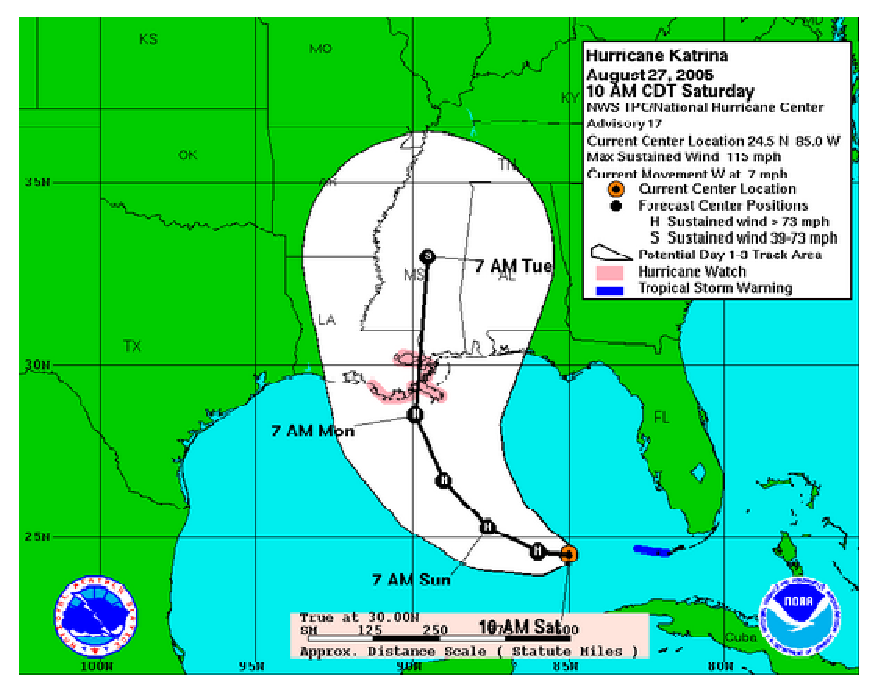
\includegraphics[width=3.0in]{figures/error_cone.eps}
       \centerline{\small The Error Cone}}
       \hspace{1em}
      \parbox[b]{3in}{
       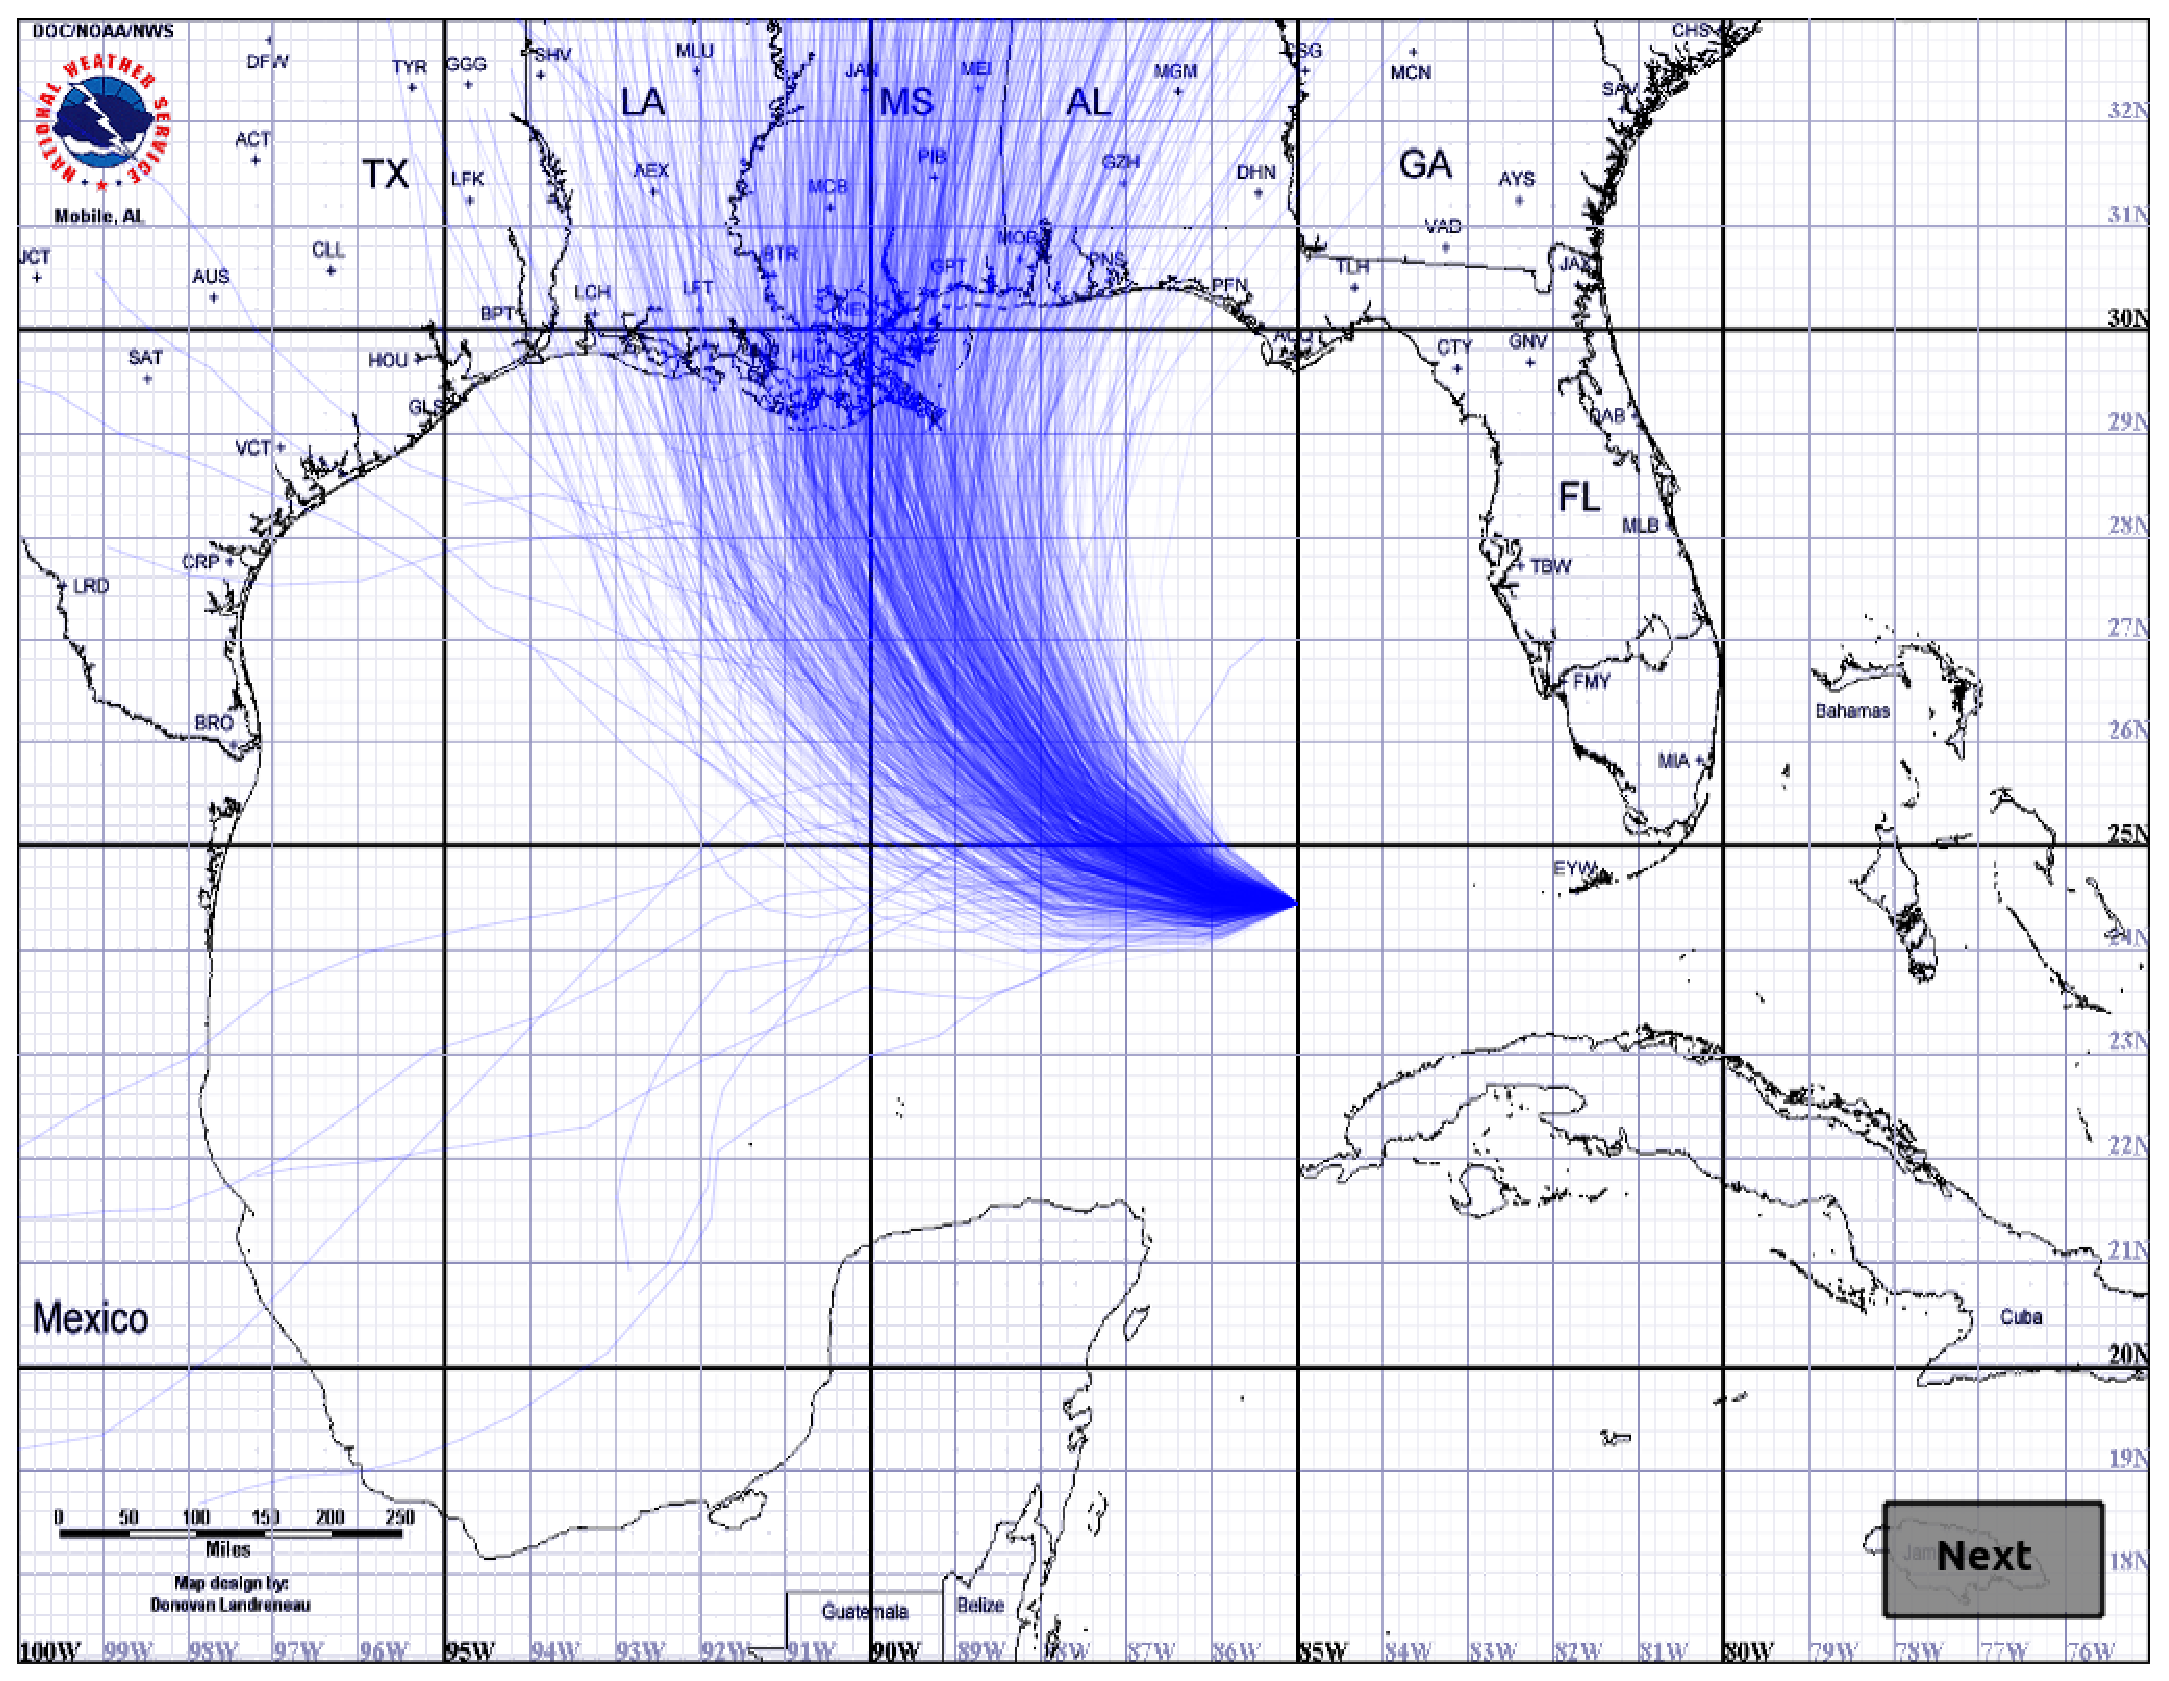
\includegraphics[width=3.0in]{figures/kat1.eps}
       \centerline{\small Our Method}}
%
%	 \subfloat[The Error Cone]{
%	   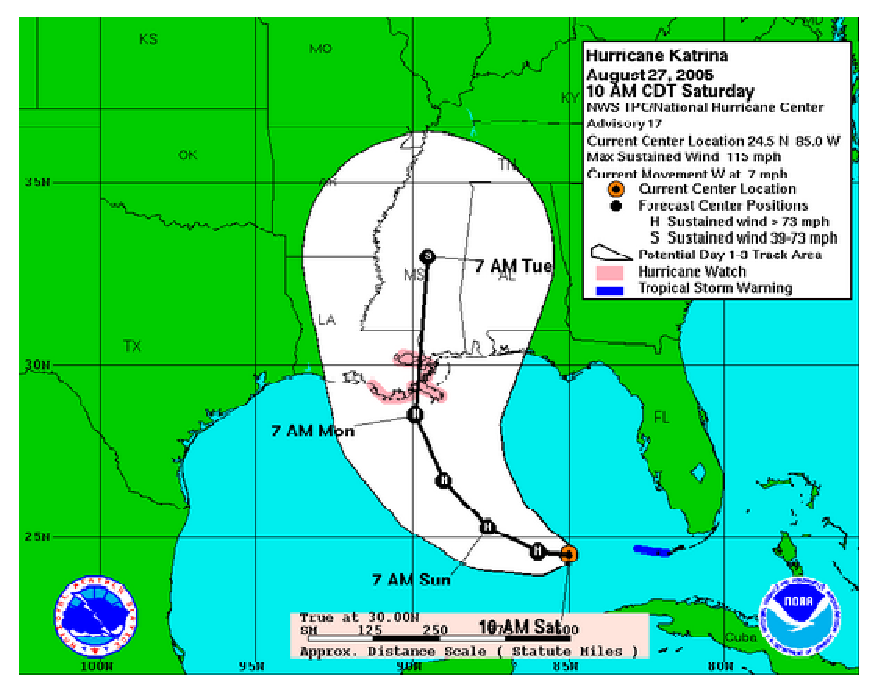
\includegraphics[width=3.0in]{figures/error_cone.eps}
%	 }
%	 \subfloat[Our Method]{
%	   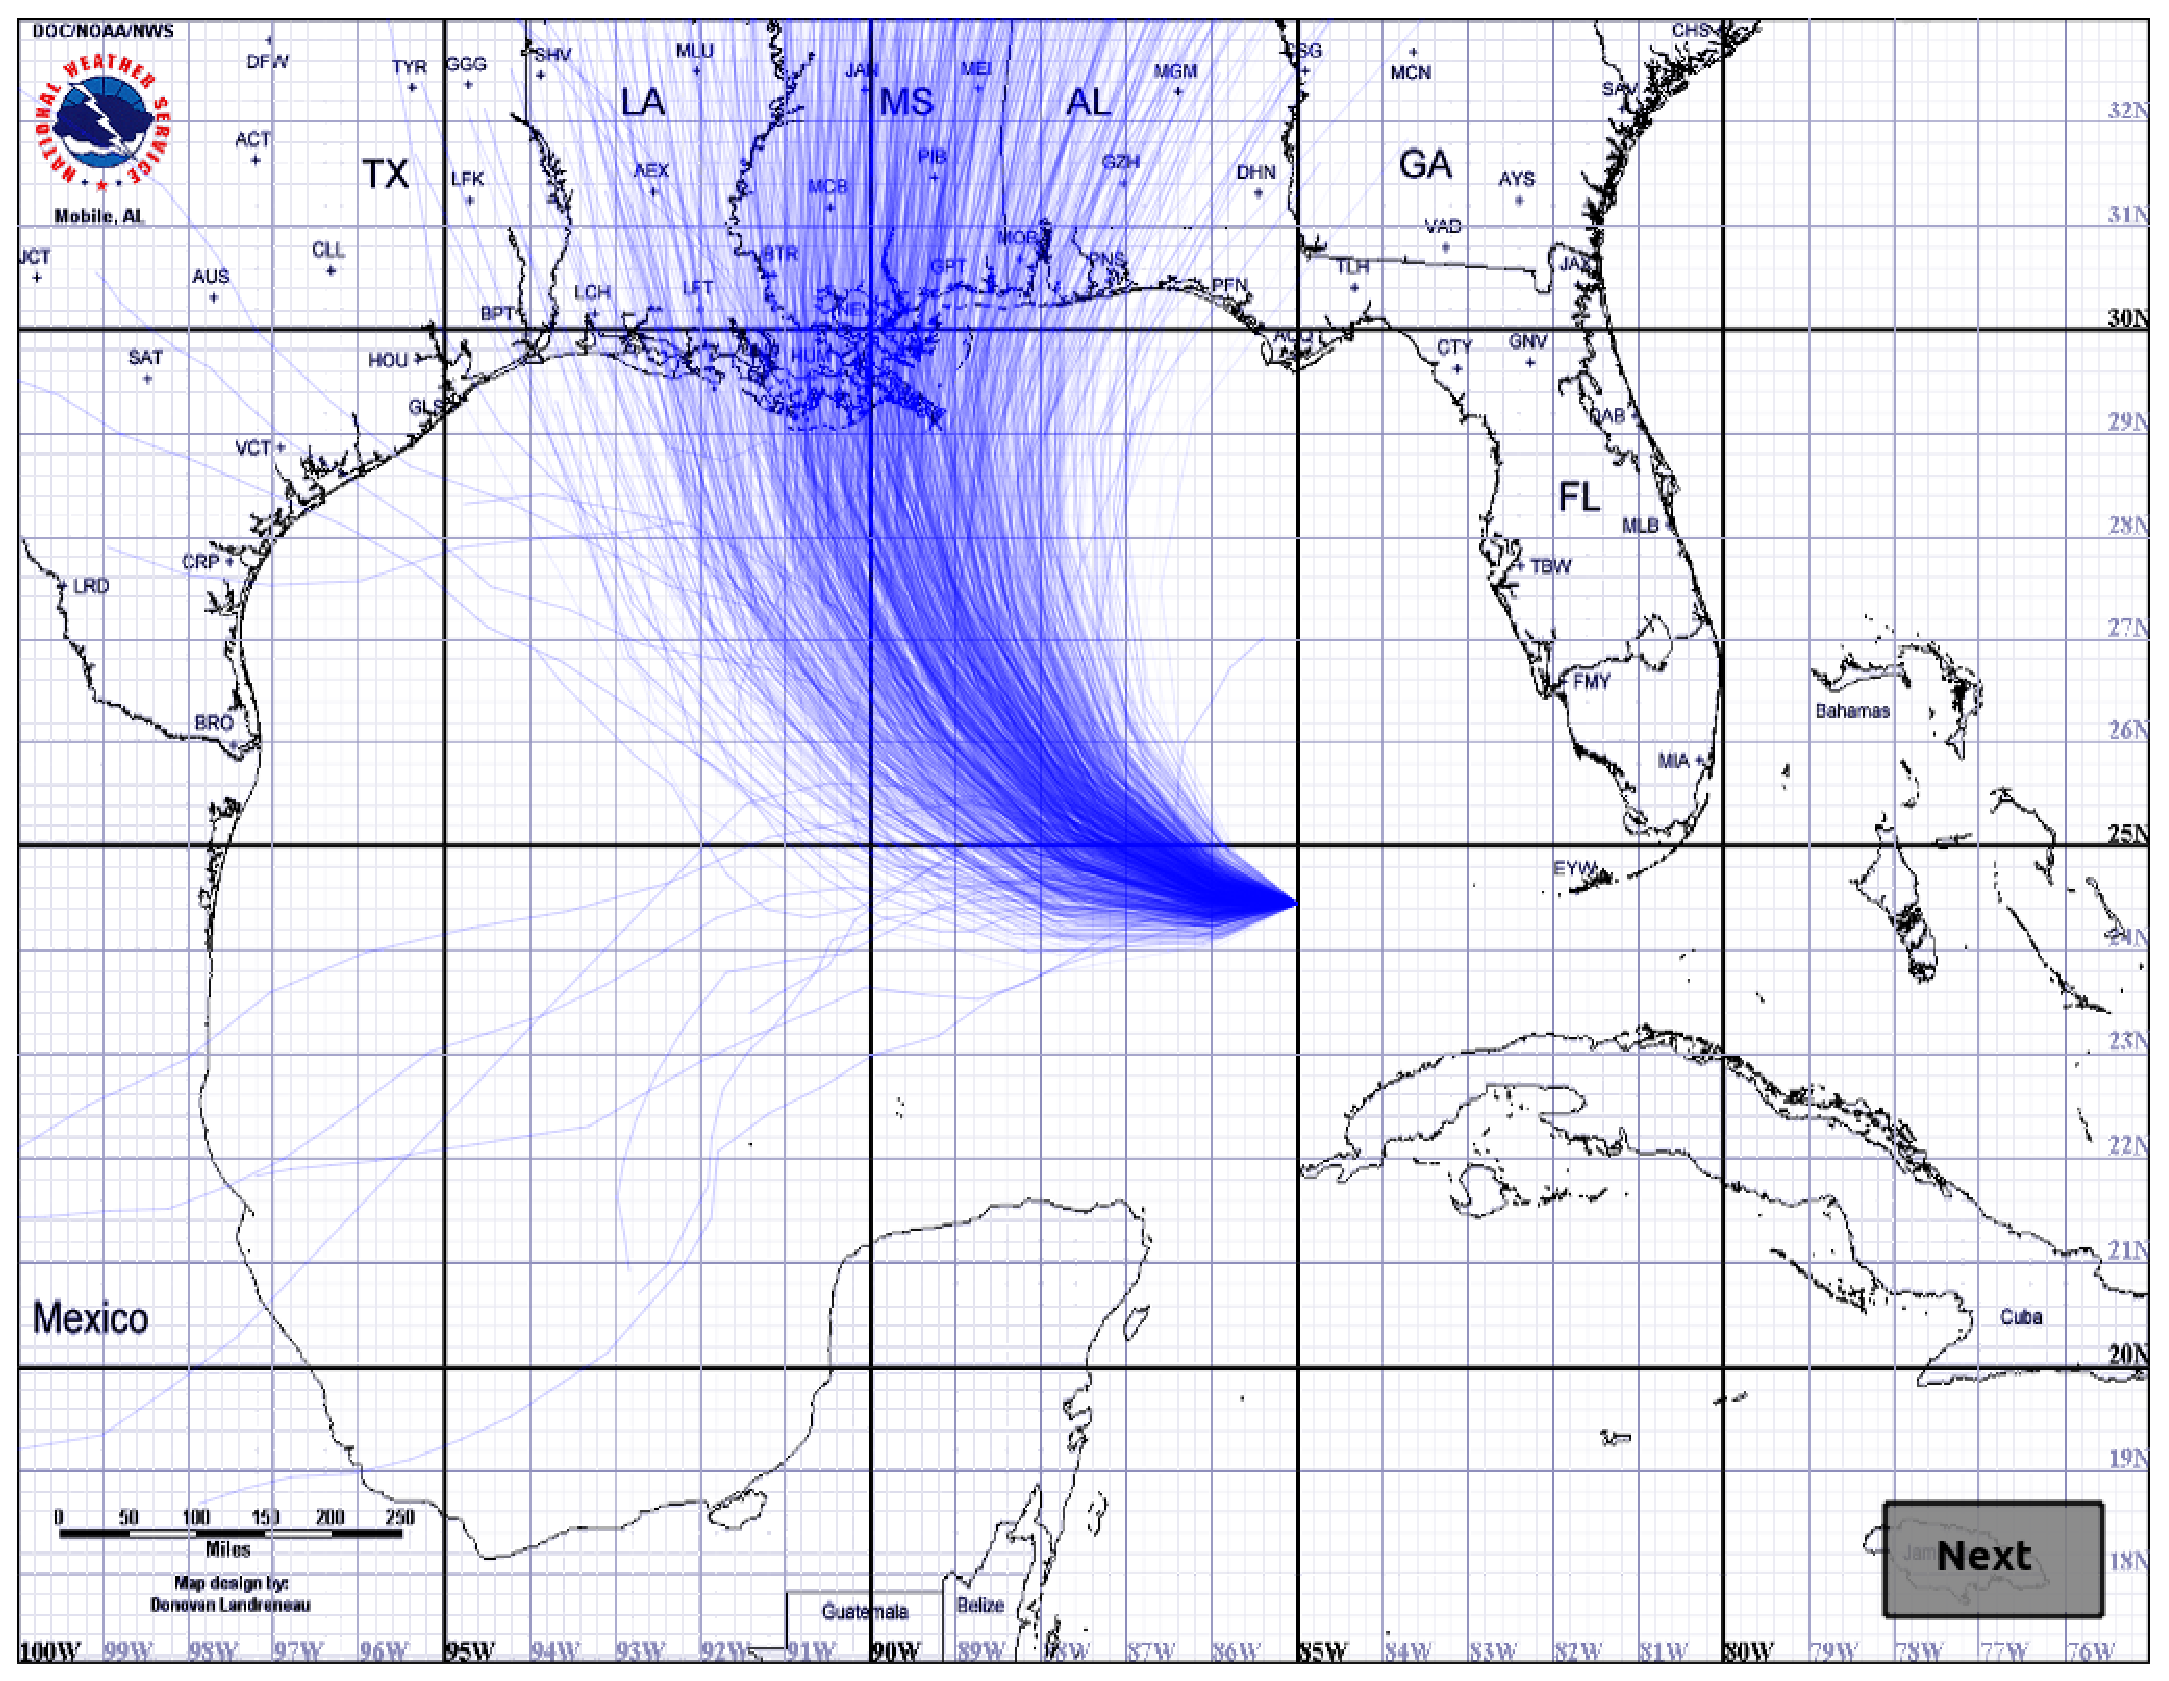
\includegraphics[width=3.0in]{figures/kat1.eps}
%	 }
 }
 \caption{Hurricane Prediction Visualization}
 \label{fig:ec}
\end{figure*}

To address these potential problems with the error cone visualization, we are investigating a new method 
that attempts to disaggregate the statistics of the error cone, in order to
show the diversity and distribution of hurricane tracks that it might subsume. Our approach uses a display
that is continuously being updated with candidate path predictions that are drawn from the distribution of likely paths
represented by the error cone.  
We generate possible hurricane tracks, which are composited over each other, and fade out with time. 
Our assumption is that this type of display will be superior to the error cone in allowing subjects to more accurately predict the likelihood of a 
hurricane to affect a particular area, as indicated by their ability to describe the strike probability distribution 
indicated by the display.

\begin{figure}
 \centering
 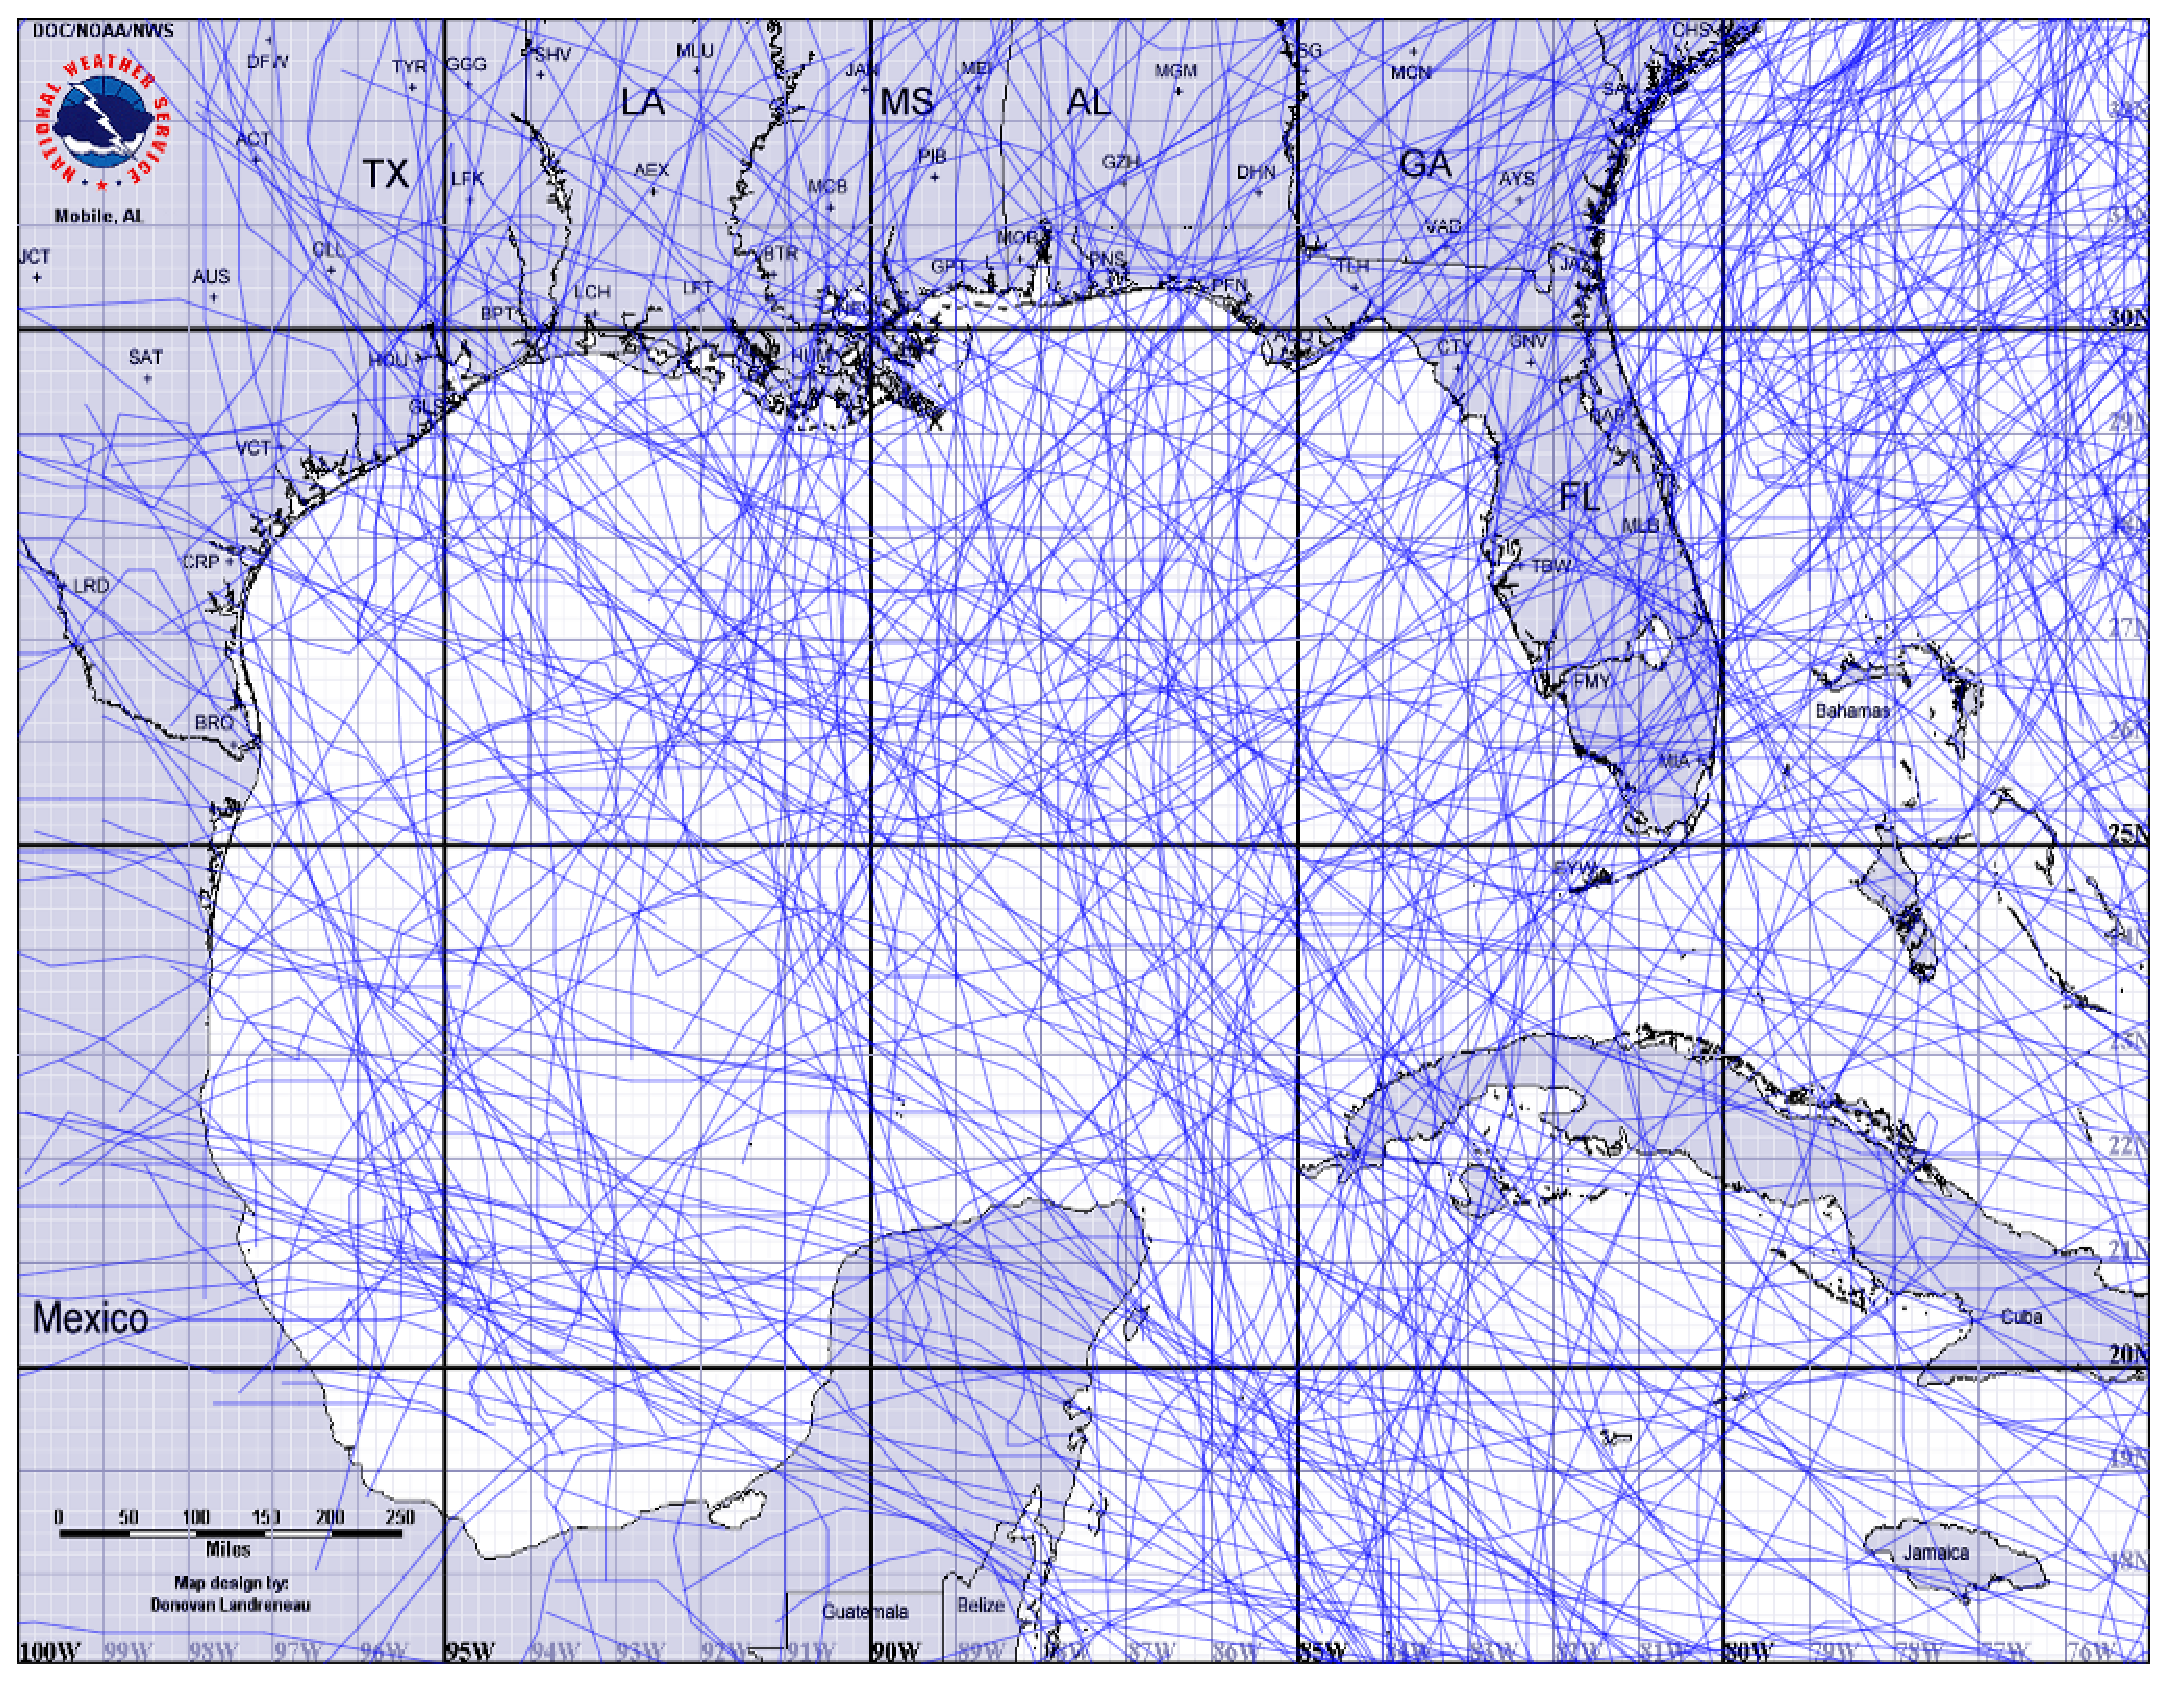
\includegraphics[width=3.0in]{figures/historical.eps}
 \caption{Historical Hurricane Tracks Since 1945}
 \label{fig:hist}
\end{figure}

The goal is to produce a display that shows a wide range of possible outcomes, while maintaining the statistical characteristics of the error cone.  Simply generating these hurricane paths according to a Gaussian distribution  about the predicted path would not be correct for two reasons.  The first is the level of diversity. 
While hurricanes often track the predicted path, extreme deviations are not uncommon.  
Fig \ref{fig:hist} shows all of the hurricane tracks in the Gulf of Mexico region since 1945.
While some patterns can be seen in this historical data, the most salient characteristic is that the behavior of individual hurricanes can vary widely.  
The second is that we have no reason to assume that the area of prediction is normally distributed.  In our work we use both the projected path of a hurricane as well as historical data to achieve a desirable level of path diversity.  


%% \section{Introduction} %for journal use above \firstsection{..} instead

\section{Background}

\subsection{Previous Studies}
Clearly visualization tools that communicate information on the parameters and uncertainties of hurricane predictions need to be designed in formats that users are able to process quickly and effectively.  While several visualization tools are available that describe the various parameters of a hurricane advisory, Broad et al.~\cite{Broad:007:MCOUF} have shown that the error cone is most widely used by officials and the general public as a means of evaluating the progress and prediction of a hurricane.  Unfortunately, an evaluation of the available products during the 2004 Florida hurricane season showed that for many the error cone was not clearly communicating the probabilistic nature of the hurricane prediction or its potential path~\cite{USACE:2004:ES}.  Not only was an inappropriate level of confidence assigned to the area within the cone, but in many cases the very nature of the cone and predicted track where misunderstood.

Despite its importance to officials and the general public, little has been done to test the interpretability or to develop alternatives that
are likely to be better understood. There has some work on other issues related to hurricane prediction. For example, Steed et al.~\cite{Steed:2009:HAI} presented an illustrated visualization method that displayed a hurricane's previous track and wind swath area by processing all of the advisories over the life of a hurricane.  Martin et al.~\cite{Martin:2008:HV2D} presented a study that examined a user's ability to effectively judge the magnitude and direction of a hurricane's winds as a two dimensional vector field. While both showed interesting results, neither visualized the uncertainty associated with a hurricane prediction as a part of their method.  We know of no other work developing alternative displays that attempts to show the natural uncertainty associated with hurricane predictions while still describing the most probable path.

\subsection{Computing Distance and Direction on the Earth's Surface}

All of the calculations used in our algorithm take into account the curvature of the Earth.  These calculations are well known \cite{Veness:2010:MVT}, but summarized here for convenience.  To conform to the standards of navigation, a bearing of $0^\circ$  is true north, and increases clockwise through $360^\circ$. Latitude is $0^\circ$ at the equator, and $90^\circ$ at the North Pole. Longitude is $0^\circ$ at the Greenwich Meridian, increasing in the positive direction to the East.
For the following formulas, $(\varphi_{i}, \vartheta_{i})$ represent the latitudinal and longitudinal coordinates of a 
point $i$ in degrees, and $R = 6371.0$ km is the radius of the Earth.

To determine the distance $d$ between two points $(\varphi_{1}, \vartheta_{1})$, and $(\varphi_{2}, \vartheta_{2})$
we use the Haversine formula,
\[
 \begin{array}{lcl}
 a &=& \sin^2(\frac{\varphi_{2}-\varphi_{1}}{2}) + \cos\varphi_{1} \cos\varphi_{2} \sin^2\frac{\vartheta_{2}-\vartheta_{1}}{2}, \\
 d &=& 2R \tan^{-1}\frac{\sqrt a}{\sqrt {(1-a)}}.
 \end{array}
 \label{eq:hav}
\]

The bearing from one point to another is given by
\[
  \theta = \tan^{-1}( \frac{\sin(\vartheta_{2}-\vartheta_{1}) \cos\varphi_{2}}{\cos\varphi_{1} \sin\varphi_{2} - \sin\varphi_{1} \cos\varphi_{2} \cos(\vartheta_{2} - \vartheta_{1})}) + 180^\circ. % \bmod 360
 \label{eq:bear}
\]
It should be noted that as a path is traveled from an initial position to a final position, the bearing will change 
continuously.

Given a starting position $(\varphi_{1}, \vartheta_{1})$, initial bearing $\theta$, and distance $d$ in km, the final
position $(\varphi_{f}, \vartheta_{f})$
is given by
\[
 \begin{array}{lcl}
  \varphi_{f} &=& \sin^{-1} (\sin\varphi_{1} \cos\frac{d}{R}) + \cos\varphi_{1}\sin\frac{d}{R} \cos\theta, \label{eq:dest} \\
  \vartheta_{f} &=& \vartheta_{1} + \tan^{-1}(\frac{\sin\theta \sin\frac{d}{R} \cos\varphi_{1}}{\cos\frac{d}{R} - \sin\varphi_{1} \sin\varphi_{f}}).
 \end{array}
\]

\section{Methodology}

\begin{figure*}[t]
 \centering
 \subfloat{
   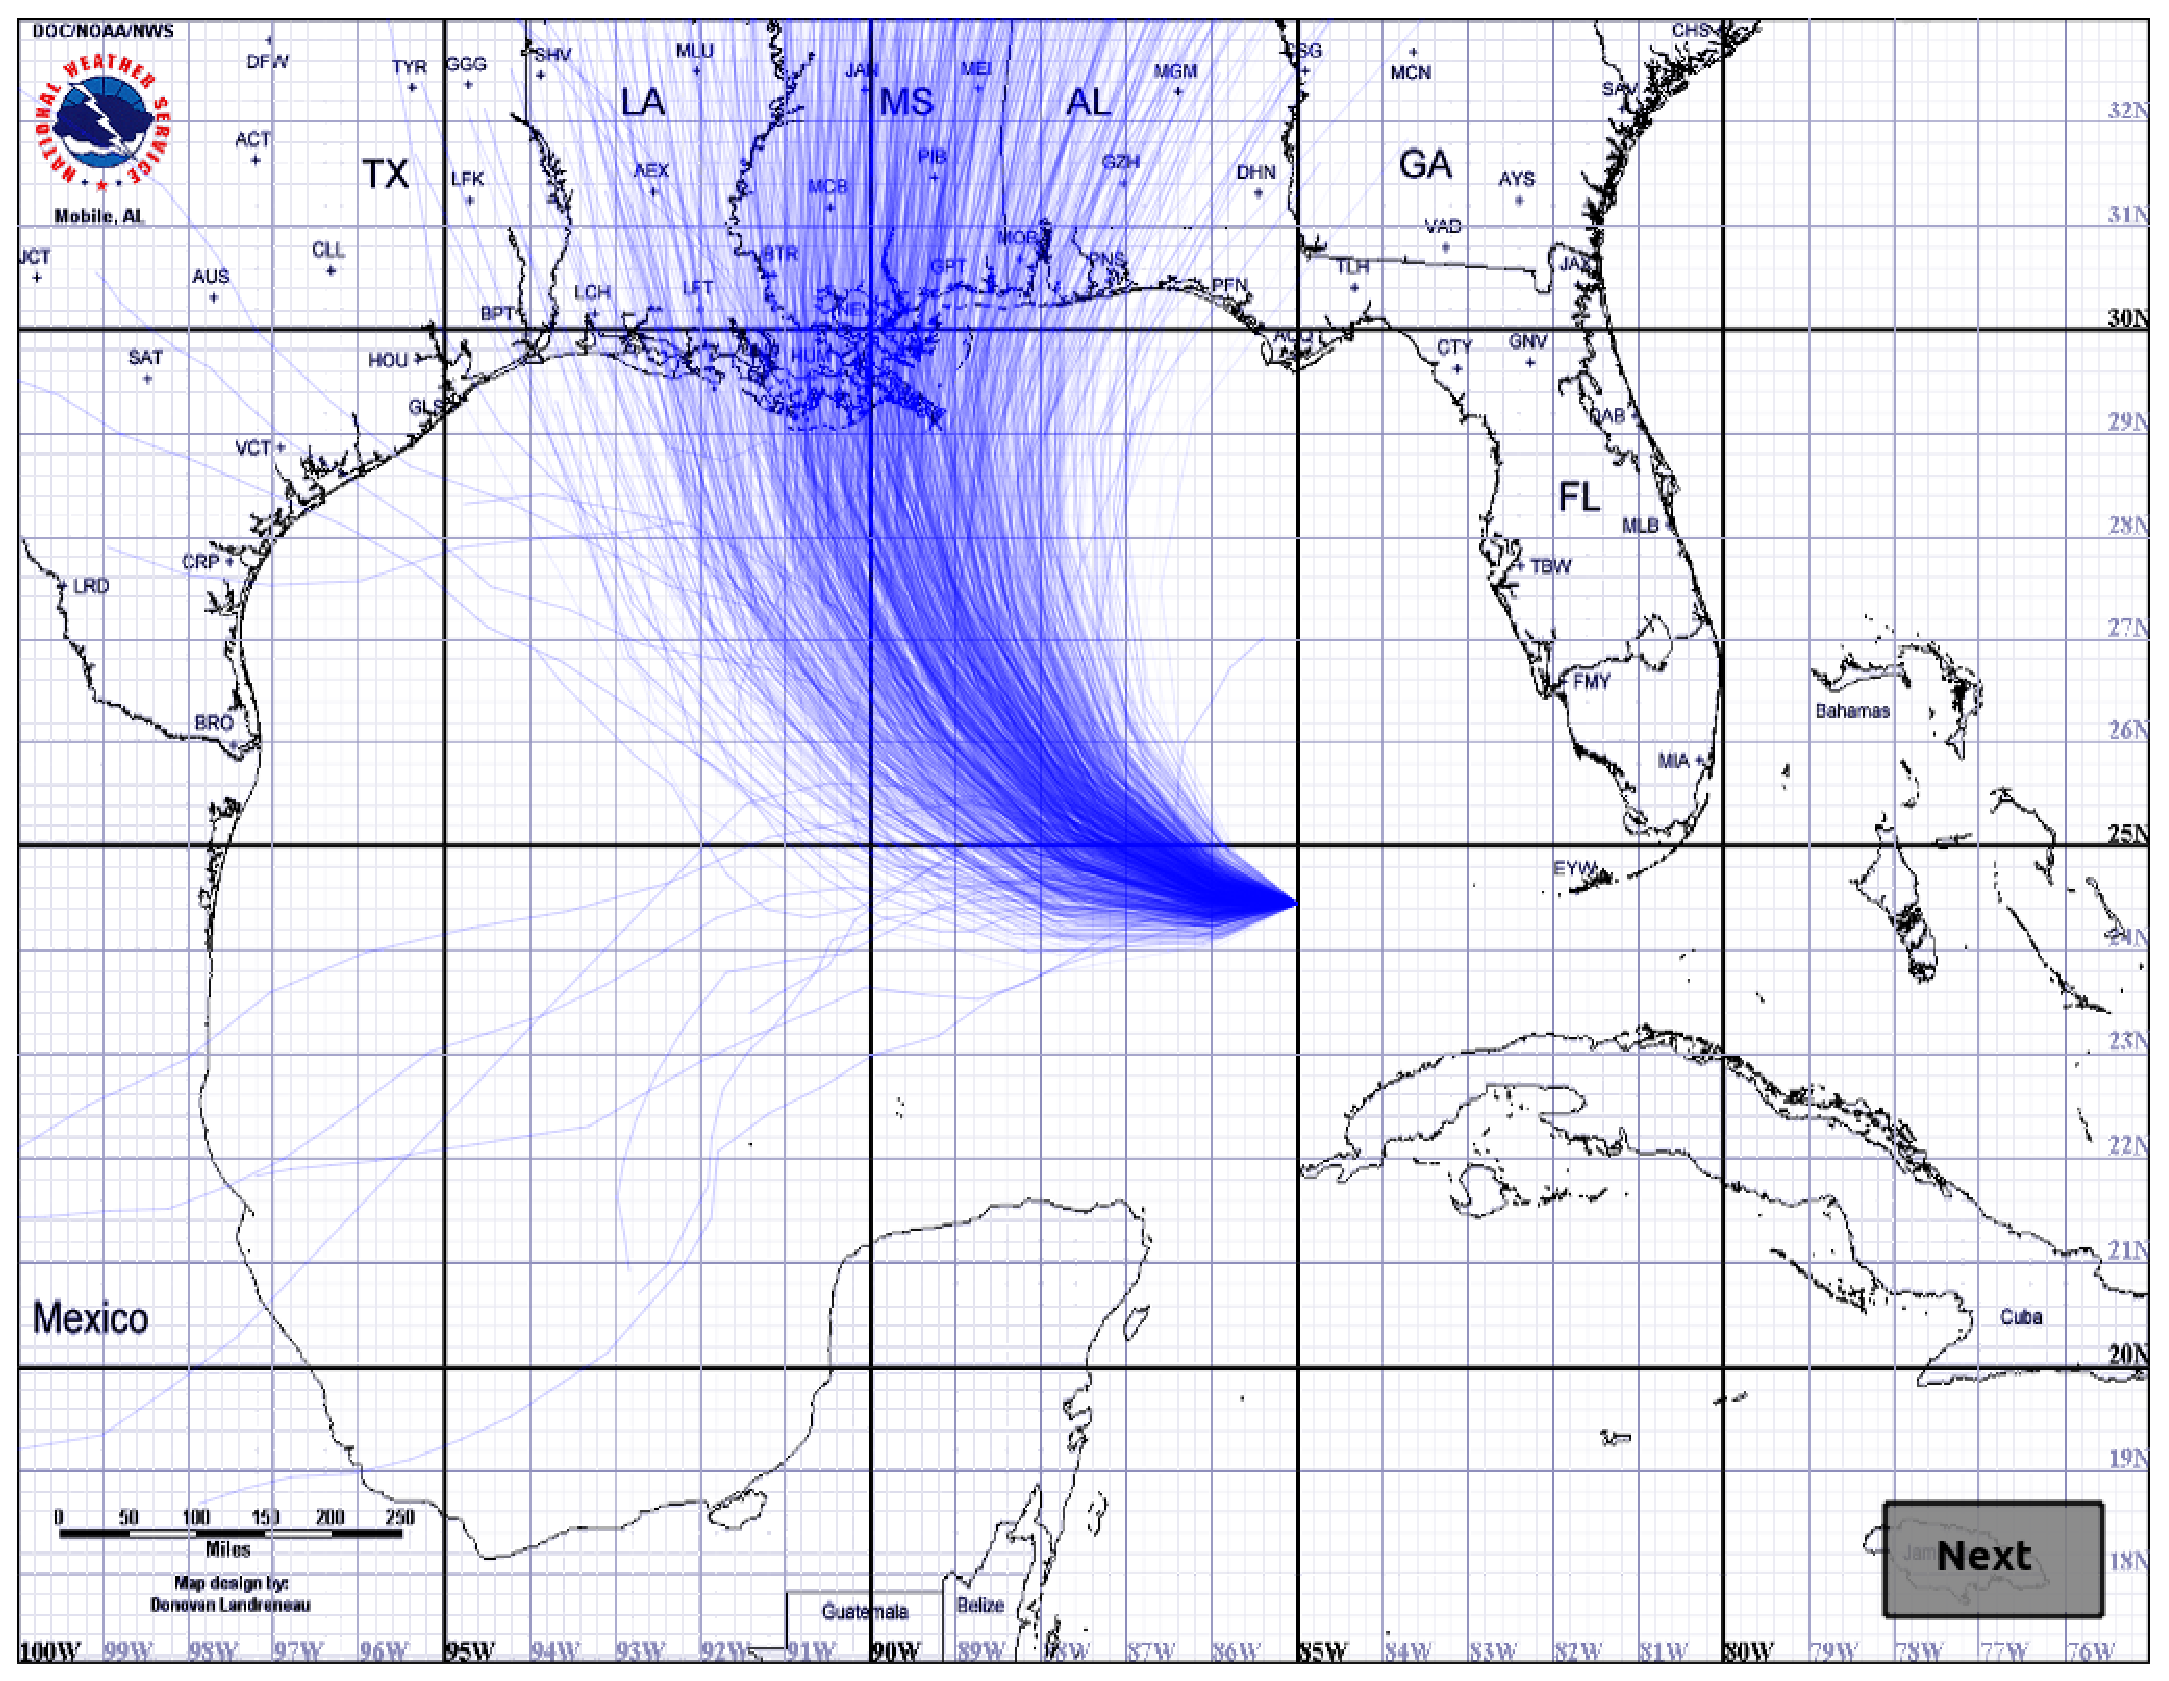
\includegraphics[width=2.0in]{figures/kat1.eps}
 }
 \subfloat{
   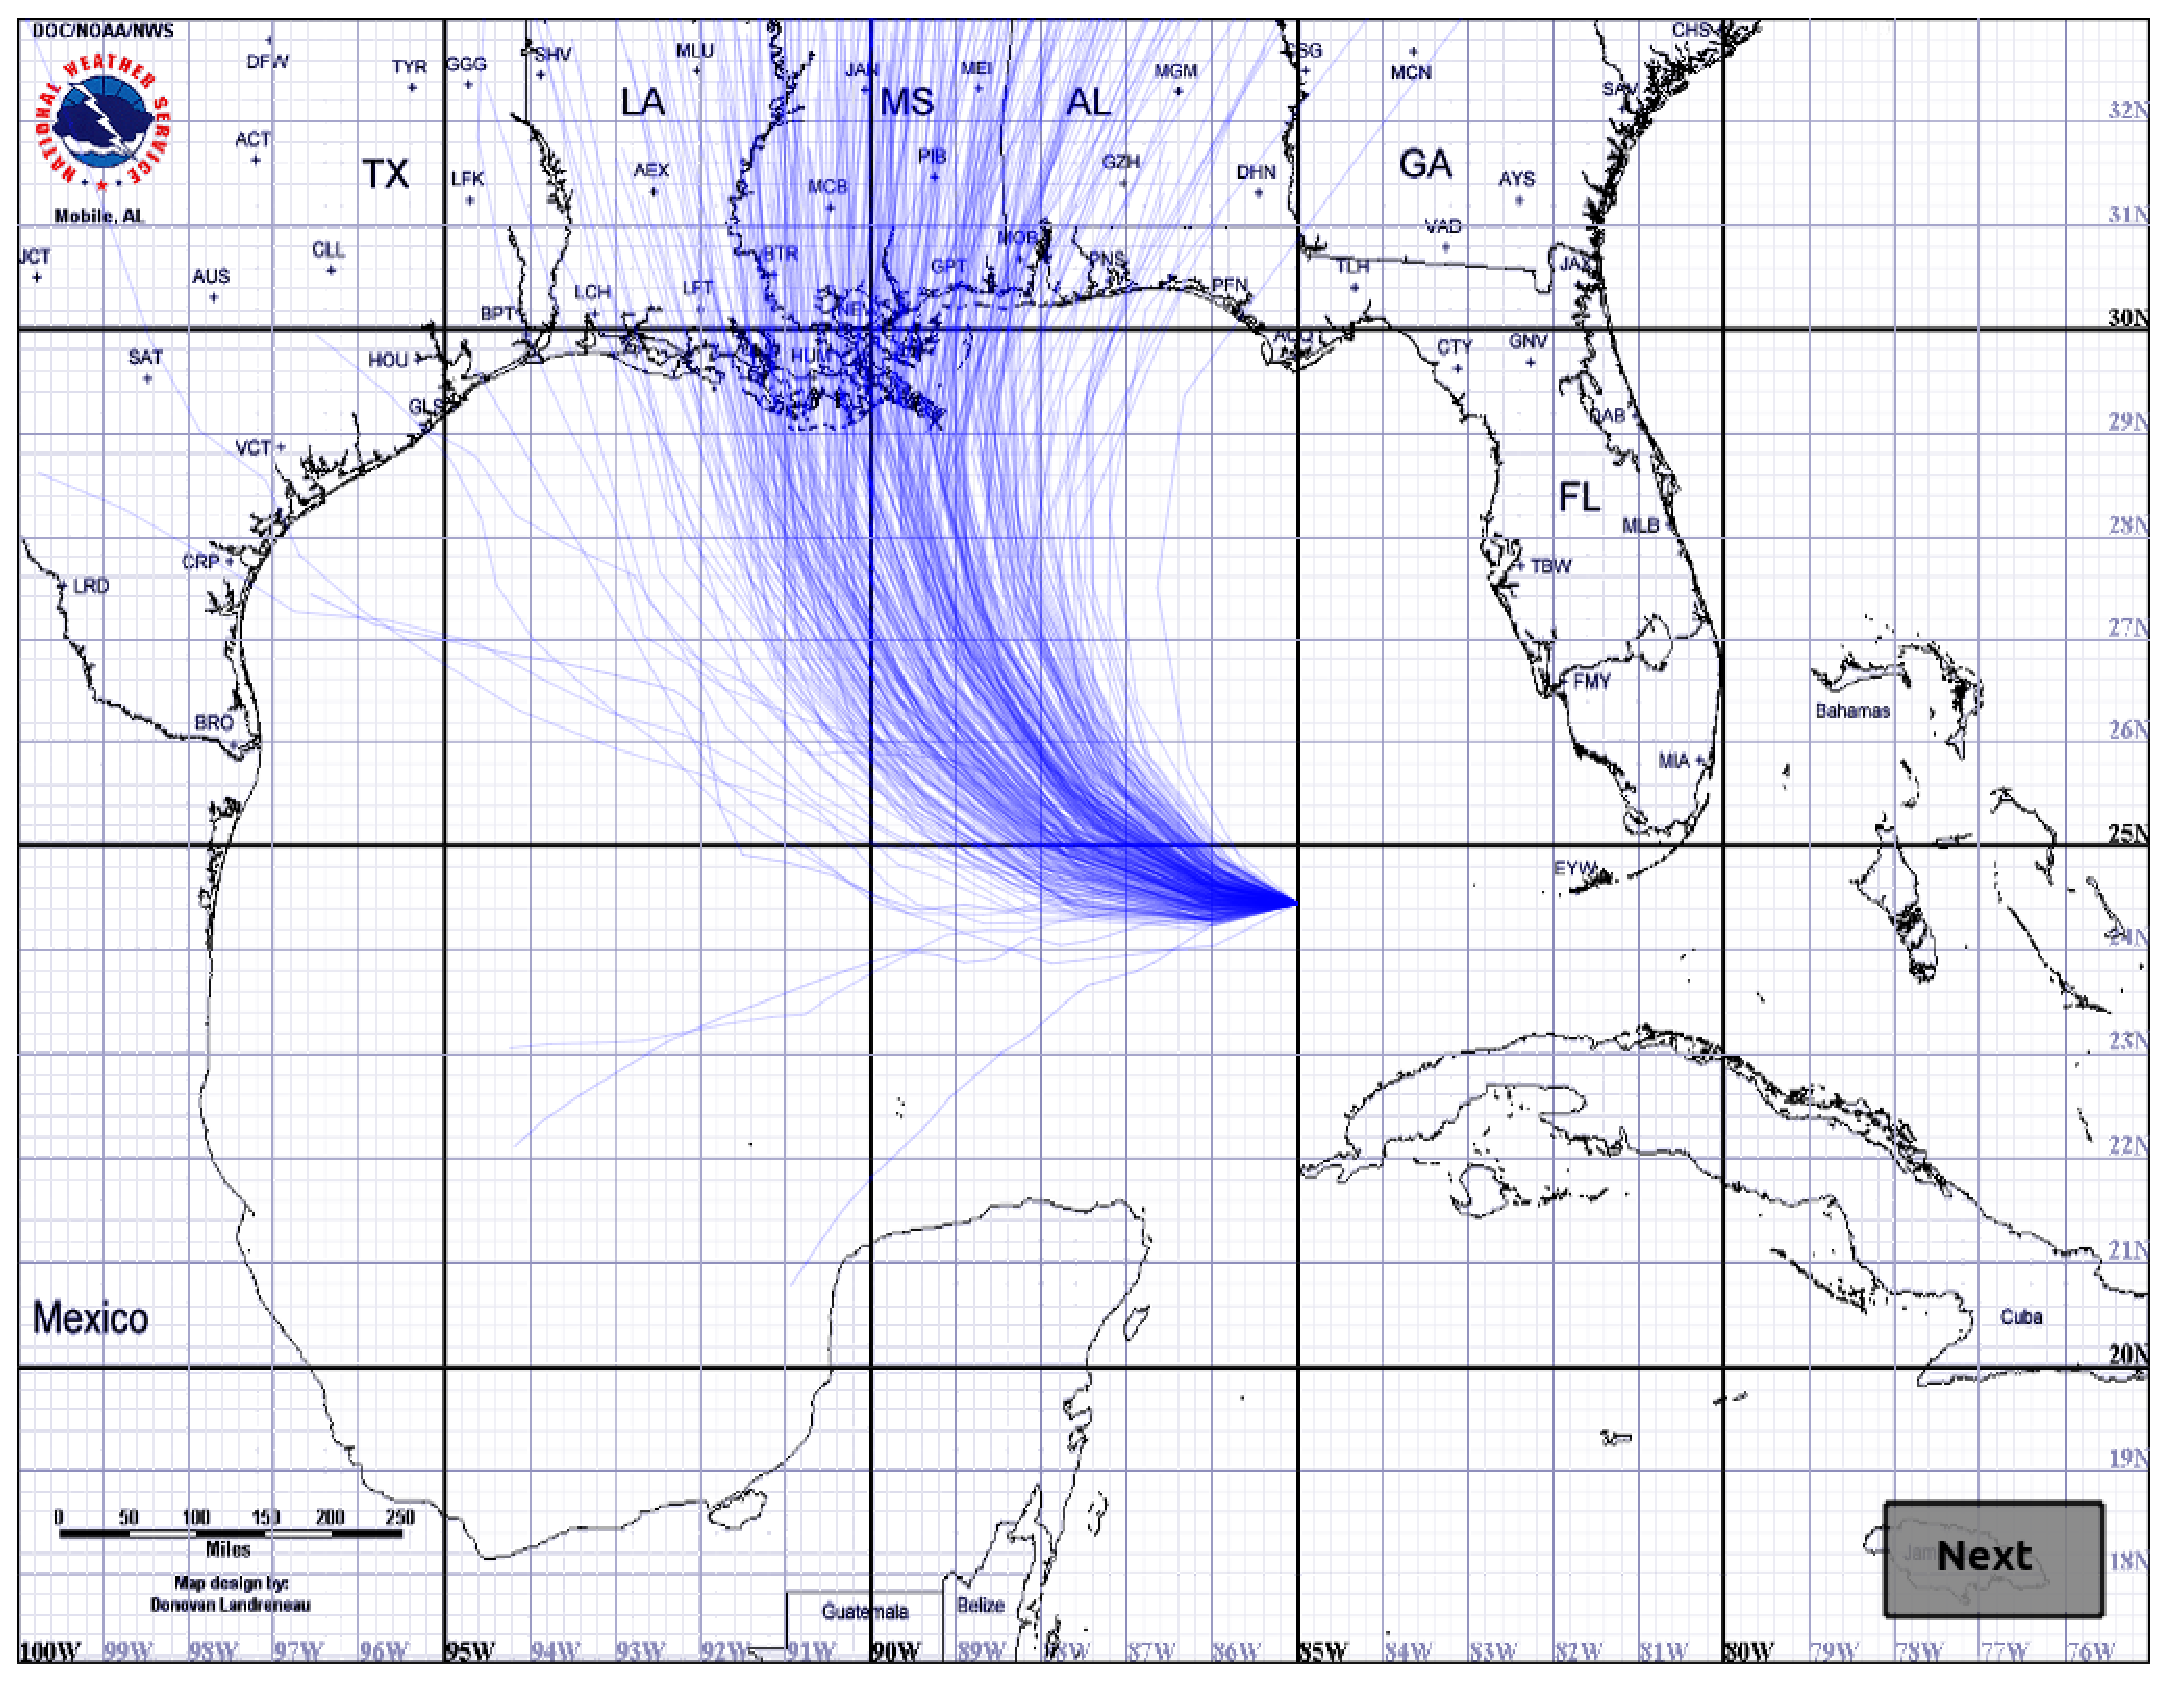
\includegraphics[width=2.0in]{figures/kat2.eps}
 }
 \subfloat{
   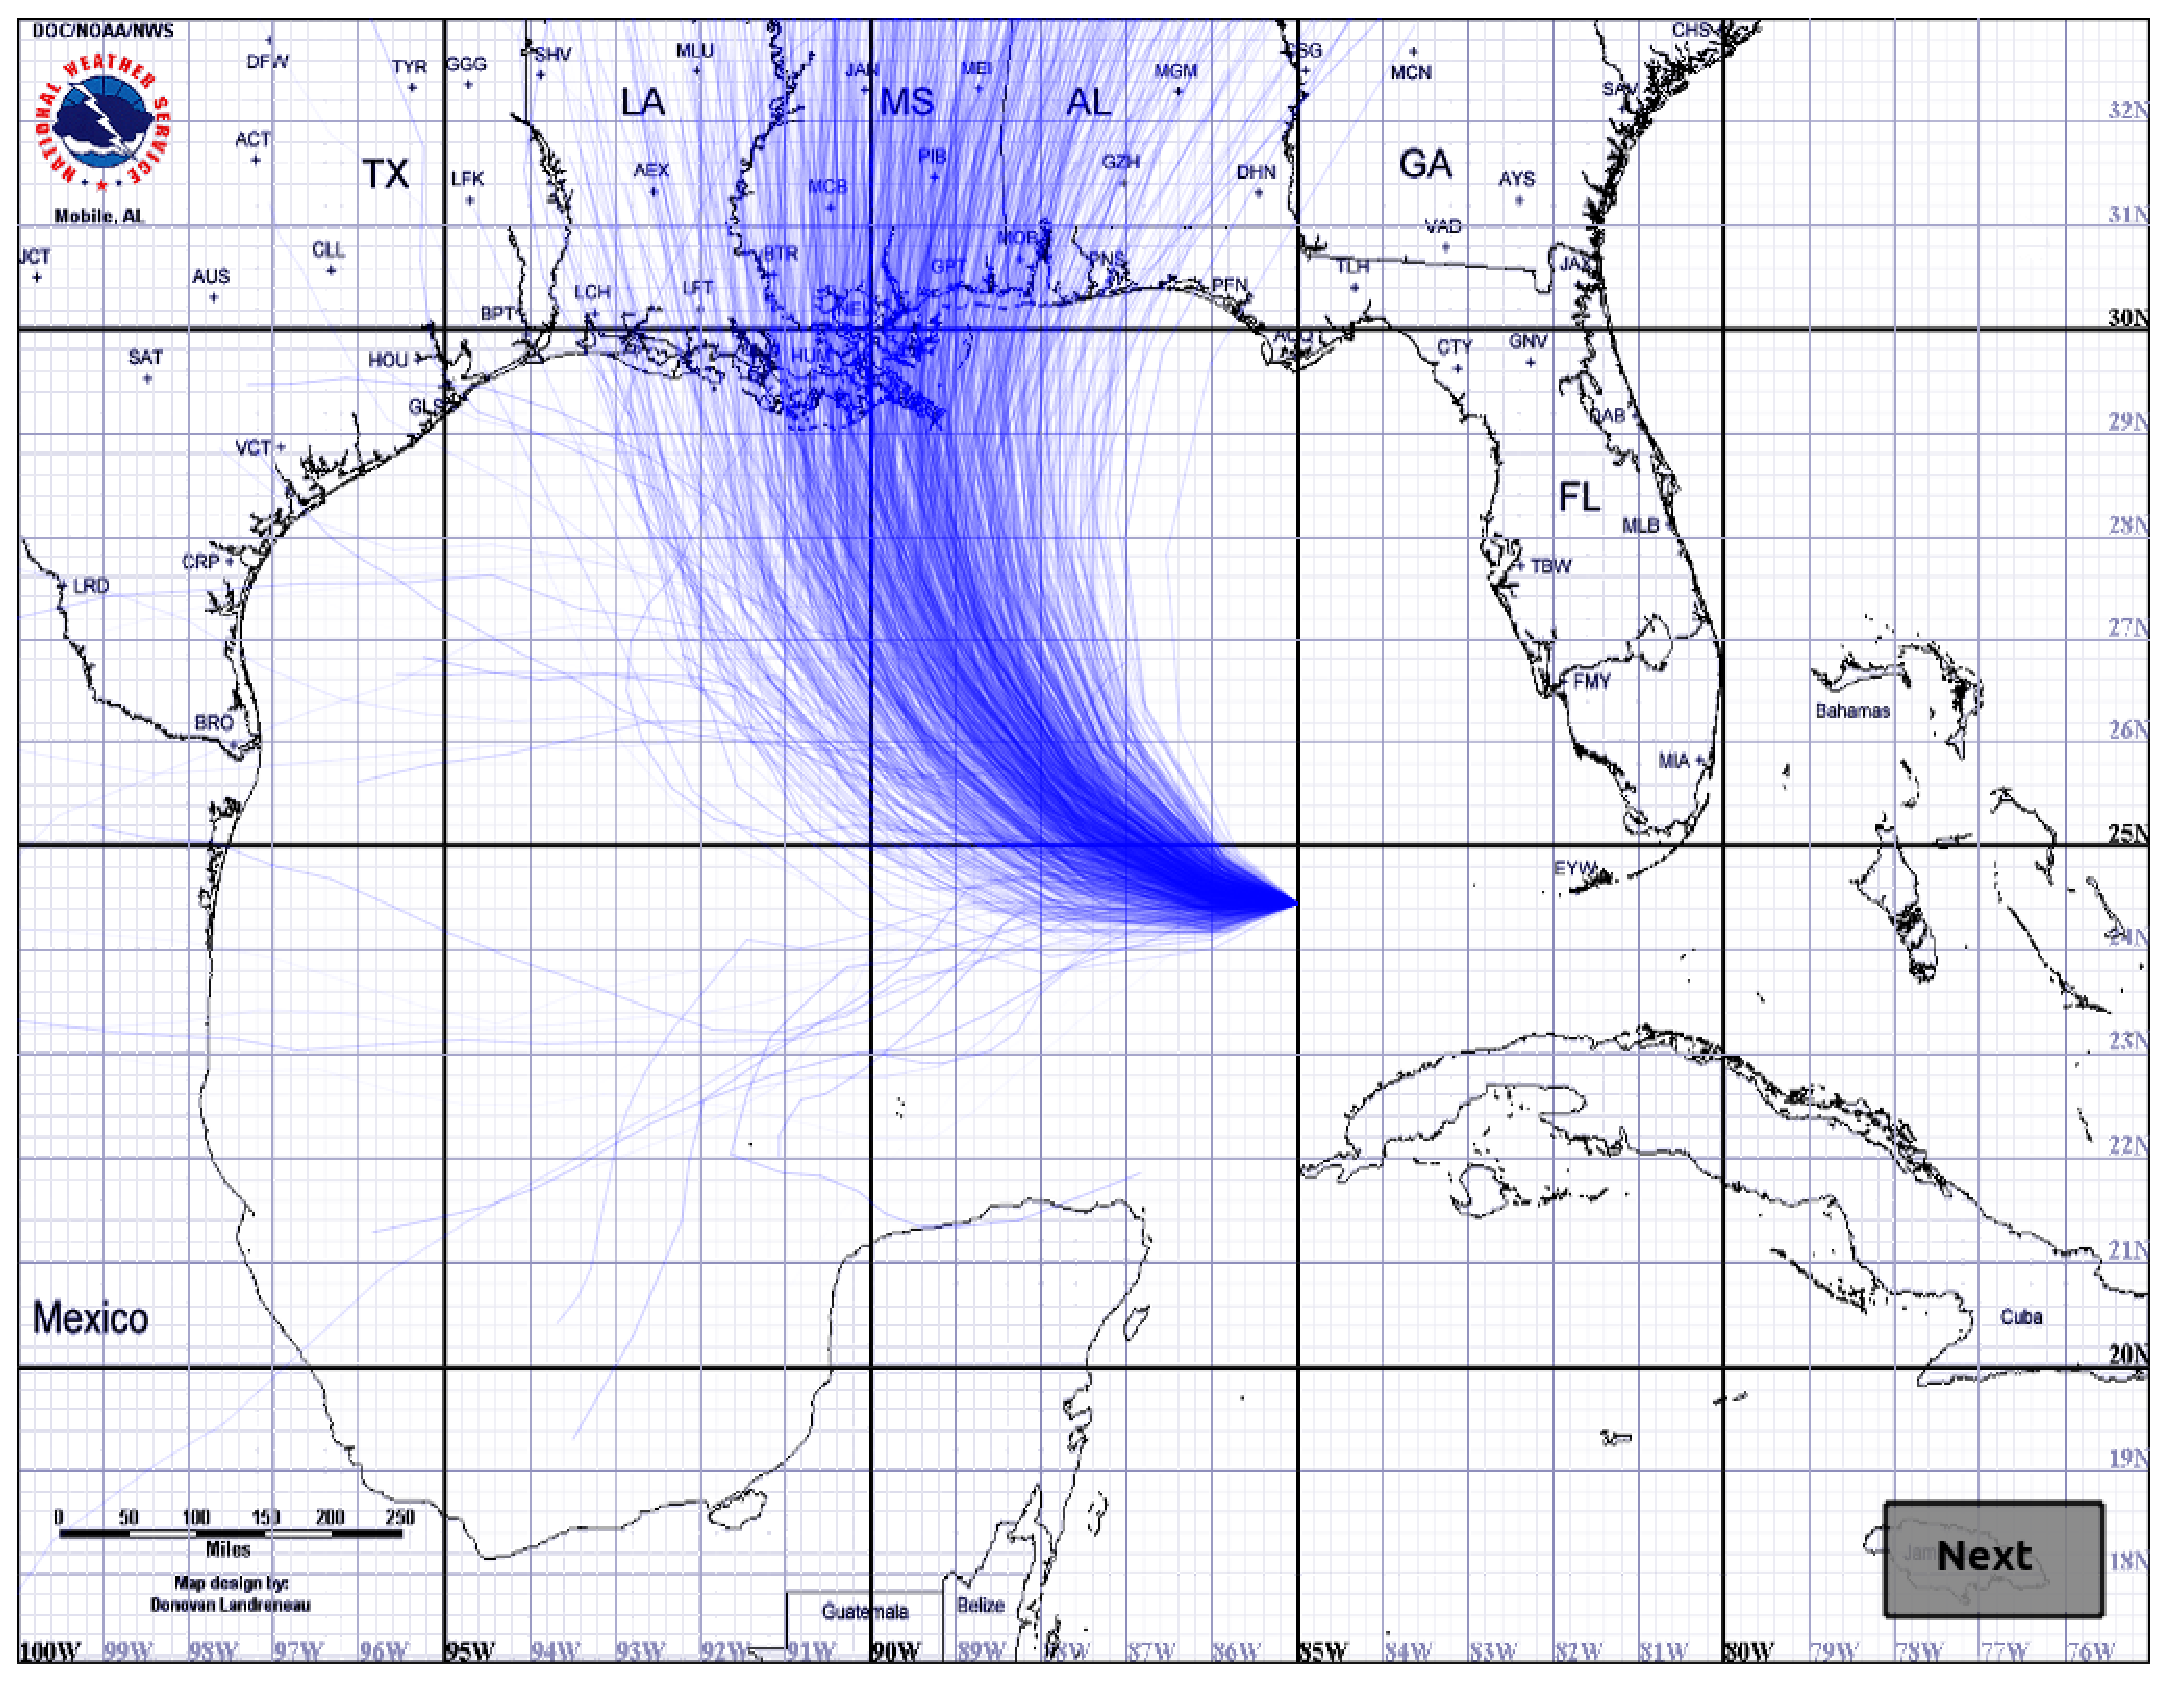
\includegraphics[width=2.0in]{figures/kat3.eps}
 }
 \caption{Our Visualization at Three Different Times for the Same Advisory}
 \label{fig:visTS}
\end{figure*}

Our method of depicting the uncertainty of a projected hurricane track uses a Monte Carlo process to repeatedly generate possible hurricane tracks.  These tracks overlay one another and fade out over time, which gives the display a changing and dynamic quality as demonstrated in the three snapshots shown in Fig \ref{fig:visTS}.  Our algorithm uses a time varying probability density to generate tracks that closely follow the predicted path, and a Markov model, determined from historical data, to generate tracks that move away from the prediction.  These are used to iteratively generate three hour sections of a track until the full track has been completed.  Each of our generated tracks is initialized to the speed and bearing at the start of the
current advisory. Once the initial speed and bearing is determined, a bearing and speed change for the next section is generated from one of our probability models.  This bearing and speed change is applied to the current speed and bearing to determine a new position.

As each path is initialized, the statistical properties of the paths already generated will help decide which of the two probability models will be used to determine the bearing and speed change for each segement of the new path.  If 68\% or more of the generated paths fit the error cone, then each segment of the path being generated has a 95\% chance of using the Markov model to determine the speed and bearing change and a 5\% chance of using the time varying probability density function.  If less than 68\% of the paths fit the error cone, then each segment of the path being generated has a 99\% chance of using the time varying probability density function to determine the speed and bearing change, and a 1\% chance of using the Markov model.

A generated path is said to fit the error cone if each point along the generated path is within a distance $d$ of the corresponding point on the predicted path, where $d$ is determined by the width of the error cone at that point. 

%While individual generated tracks are not constrained to stay within 
%the error cone, the overall statistical properties of our set of generated 
%paths closely match those of the error cone.

The rest of this section describes how the predicted path and historical data are each used to generate the 
speed and bearing changes that are applied to each path segment.

\subsection{Using Predicted Data}

In order to use the prediction from the current advisory for path generation,
we treat the prediction as a time varying probability density function
\[
  p(\Delta \theta, \Delta s | t; \Delta t),
\]
where $\Delta \theta$ is a random variable representing bearing change, $\Delta s$ represents speed change,
$t$ is time since the beginning of the advisory, and $\Delta t$ is a parameter for the time step over which 
change takes place.
We discretize the
time axis, yielding a set of fixed probability density functions of the form
\[
  p_{t}(\Delta\theta, \Delta s; \Delta t),
  \label{eq:pre_fin}
\]
where $t$ is the time at the start of a segment.  
%These are built for 
%every section of the predicted path and indexed accordingly when it is decided that predicted information 
%should determine $\Delta\theta$ and $\Delta s$.

In order to build these time indexed density functions, we use the prediction data contained in the advisory.
At each time step available in the prediction, we determine two corresponding points on the perimeter of the
error cone.
While the advisory provides location information for several points along the predicted path, the only 
initial information for the error cone is its width at specific points, which is determined by the 
National Hurricane Center on a yearly basis.  
Given a point on the predicted path, the corresponding points on the two sides of the error cone are uniquely
determined by the width of the cone if we measure out this distance at a bearing of $90^\circ$ from the
predicted path.
Linear interpolation is used on the predicted path and on the perimeter of the error cone to find sample 
points along each at three hour segments. The final bearing, initial bearing and speed at each of these points 
is then calculated.
To find these values, we look at three consecutive points on a path segment, $p_{i-1}$, $p_{i}$, and $p_{i+1}$.  
The speed at point $p_{i}$ is calculated by finding the distance from $p_{i}$ and $p_{i+1}$ and dividing by the 
number of hours in the segment (3 hours in our study).   Fig \ref{fig:bearing} shows how the change in bearing $\Delta\theta$ is computed from these points.  The final bearing $\theta_f$ for $p_{i}$ is found by taking the bearing 
from $p_{i}$ to $p_{i-1}$, and adding $180^\circ$.  The initial bearing $\theta_i$ for $p_{i}$ is the bearing 
from $p_{i}$ to $p_{i+1}$.  The bearing change at each point is just the minimal angular difference between the final bearing and initial bearing.  The speed change is the speed difference between $p_{i}$ and $p_{i-1}$.
These speed and bearing changes are then used to make a probability density function for the bearing change and for the speed change at each of the three hour marks of our advisory.  
\begin{figure}[htb]
 \centering
 \includegraphics[width=1.5in]{figures/bearing.eps}
 \caption{Initial Bearing and Final Bearing}
 \label{fig:bearing}
\end{figure}

We approximate the probability density function governing bearing change at each time step by estimating
the probabilities of a small set of bearing changes, and interpolating between them. In our work we are using 101 samples.  The central sample value $c$ is set to the bearing change of the corresponding point on the predicted path.  The minimum and maximum bearing changes sampled are
\begin{equation}
 \begin{array}{lcl}
  m &=&  c + 1.5 (\min(\Delta \theta_{l}, \Delta \theta_{r}) - c), \\
  M &=&  c + 1.5 (\max(\Delta \theta_{l}, \Delta \theta_{r}) - c), \\
  \end{array}
 \label{eq:pre_samples}
\end{equation}
where $\Delta \theta_{l}$ and $\Delta \theta_{r}$ are the bearing changes on the left and right sides of the error cone at the current time.  Half of the remaining samples are evenly spaced from $m$ to $c$ with the other half evenly spaced from $c$ to $M$. Equation \ref{eq:pre_samples} provides a support that is 1.5 times the distance between the minimum and the maximum bearing changes, giving support outside the error cone.  Note that the distance between the samples on the lower half of the distribution will generally not be the same as the distance between the samples on the upper half.

The probabilities corresponding to each sample are estimated as
\[
 \begin{array}{lcl}
  p(\Delta \theta) = \frac{1}{\sigma\sqrt{2\pi}} e^{\frac{-(\Delta \theta-c)^2}{2\sigma^2}},
 \end{array}
 \label{eq:pre_weights}
\]
where $\Delta \theta$ is the sample value, the standard deviation $\sigma$ is set to $(c-m)/3$ if the sample bearing change is less 
than $c$ or set to $(M-c)/3$ if it is greater than $c$. This gives a distribution on each side of the predicted path that reaches two
standard deviations at the error cone edges. Once the probabilities of each of  the samples have all been found, the set of 
samples is scaled so that the total area under the curve, estimated using the trapezoidal rule, is 1.0.  Fig \ref{fig:ndf_pre} shows an example distribution shape, which will typically not be Gaussian.
\begin{figure}[htb]
 \centering
 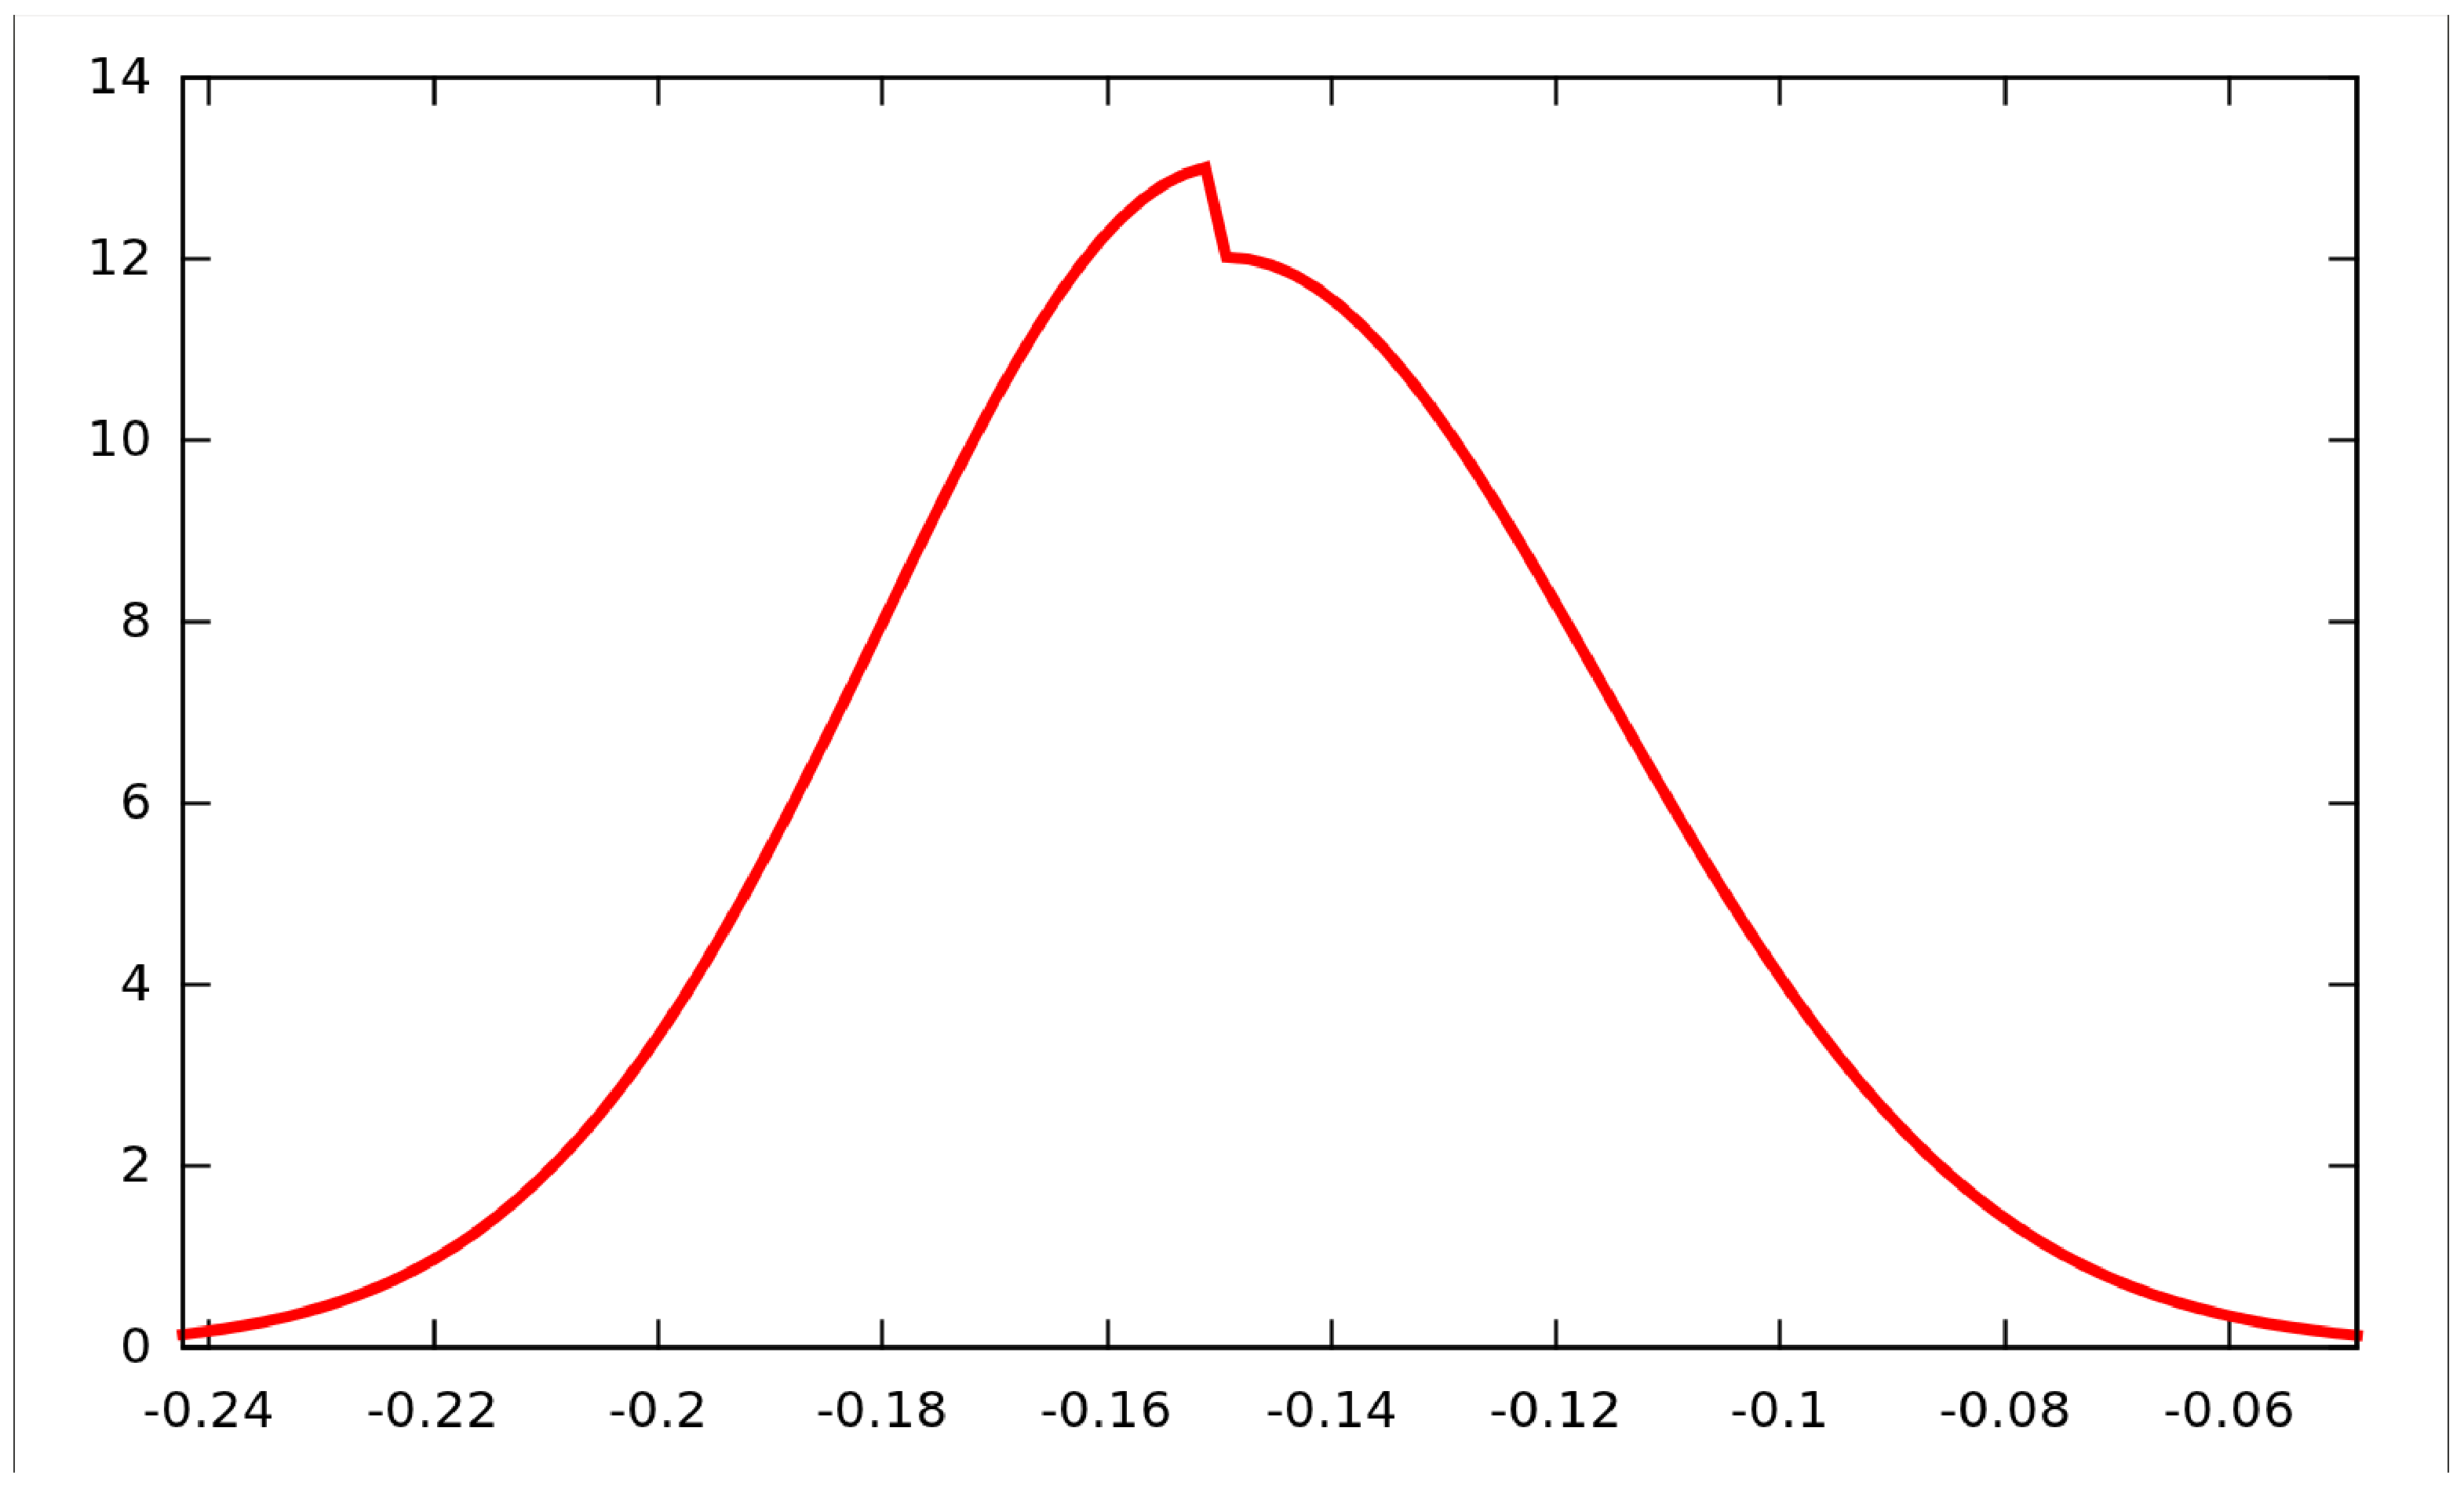
\includegraphics[width=3.0in]{figures/ndf_pre.eps}
 \caption{Time Varying Probability Density Function Using Predicted Path Data}
 \label{fig:ndf_pre}
\end{figure}

When using the predicted data to generate the bearing and speed change for a given segment, the appropriate probability density function is indexed by the current time. We generate a random number from 0 to 1, numerically integrate the probability density function using the trapezoidal rule until the integration reaches this number, and return the corresponding bearing.

Speed change is determined similarly, with the exception being the computation of $m$ and $M$.  To include speed changes that allow for the generated hurricane tracks to reach the full range of area inside the error cone, these equations have been modified to
\begin{equation}
 \begin{array}{lcl}
  m &=&  c + 3.0 (\min(\Delta \theta_{l}, \Delta \theta_{r}) - c), \\
  M &=&  c + 3.0 (\max(\Delta \theta_{l}, \Delta \theta_{r}) - c), \\
  \end{array}
 \label{eq:pre_samples_speed}
\end{equation}


The use of the probability density function allows us to generate speed and bearing changes that tend to create paths falling within the error cone, with highest density near the center of the cone.

\subsection{Using Historical Data}

\begin{figure}
 \centering
 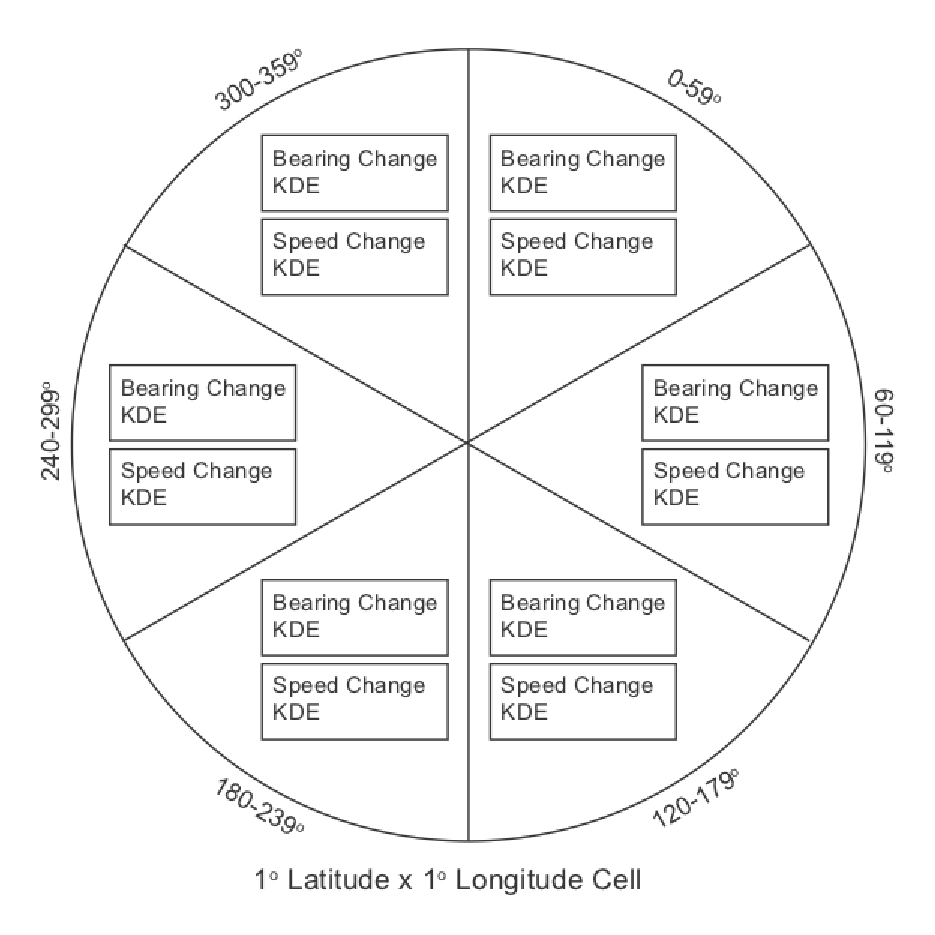
\includegraphics[width=3.0in]{figures/DataStruct-round.eps}
 \caption{Historical Data Grid Cell Structure}
 \label{fig:ds}
\end{figure}

Unlike our treatment of the predicted data, we represent the history of hurricane paths with a Markov model, which
we use to determine bearing and speed changes given a hurricane's current location, speed and bearing.
If the bearing change random variable is $\Delta\theta$ and the speed change random variable is $\Delta s$,
such a model would be summarized by the conditional probability density function
\[
  p(\Delta\theta, \Delta s | \theta, s, \varphi, \vartheta; \Delta t),
\]
where $\theta$ is the current bearing, $s$ is the current speed, $\varphi$ is the current latitude, $\vartheta$ is the current longitude, and $\Delta t$ is a time-step parameter.

In our current method, we make the assumption that change in direction and speed are independent of the
hurricane's current speed, reducing the conditional probability to
\[
  p(\Delta\theta, \Delta s | \theta, \varphi, \vartheta; \Delta t).
\]
This means that when we consider historical hurricane tracks in building our model, we need only concern
ourselves with the position of the hurricane and its current bearing.
In this way we attempt to preserve spatially local patterns found in past hurricane activity.

This conditional probability specifies two continuous three dimensional functions, which we discretize, first by sampling over spatial grid cells, each representing one degree of latitude and one degree of longitude, and then by bearing, assigning a set of six bins to each grid cell, each covering $60^\circ$. We capture this discretization by constructing a two dimensional data structure over the Gulf coast of the United States, where the cells can be represented as a rectangular grid on a Mercator Projection map. Thus, the probability density functions at cell $(i, j)$, for hurricane paths with bearing in the angular range $k$ are given by
\[
 p_{ijk}(\Delta\theta, \Delta s; \Delta t).
\]
We estimate these functions for each angular bin, by noting the bearing and speed of each historical path as it enters the grid cell, the time it spends in the cell, and its bearing and speed when it leaves the cell. Each entrance and exit constitutes one sample, which we use to construct kernel density estimators for the bearing
and speed changes. The resulting data structure has entries of the form shown in Fig \ref{fig:ds}.

\begin{figure}
 \centering
 \includegraphics[width=3.25in]{figures/histPathProp.eps}
 \caption{Propagation of a Historical Path}
 \label{fig:pathProp}
\end{figure}

  Although historical hurricane track data is available back to 1851, in our work we use only data starting from 1945 due to concerns relating to the validity of earlier measurements.  Because this data is generally too sparse to provide adequate samples for our kernel density estimators, we generate three supplemental parallel paths on each side of every historical path, as shown in Fig.~\ref{fig:pathProp}.  The parallel paths are created by stepping along each point of a historical path while generating three corresponding points at 60 km intervals in both directions perpendicular to the historical path.
%The data structure is initially populated so that each bin in each grid cell contains a probability density function representing the historical hurricanes that pass through the grid cell at bearings that correspond to the particular bin.  
To assure that actual historical paths have a greater contribution to the probability density function than 
the parallel tracks, every path is assigned a weight value $w$, with original historical paths having weight 1.0 and the parallel paths having weights $0.75$, $0.5$, and $0.25$.

%All of the paths are processed to build the probability density functions for each bin in each grid cell.  We begin by using the intersection points of each path with the edges of the grid cells to measure the bearing and speed changes along that path. 
%Initially, the data structure stores the changes in bearing and in speed a hurricane experiences from the point that it enters a grid cell to the point that it leaves.  The bin that this information is stored in is determined by the bearing of the hurricane as it enters the grid cell.
All of the historical and supplemental paths are intersected with the spatial grid cells, and used to construct two kernel density estimators for every bin in each grid cell.  These approximate the two required probability density functions governing bearing change and speed change. Because the point at which a hurricane enters and leaves a grid cell, as well as its bearing and speed at these respective points, is not directly available to us through the historical records, we determine them using linear interpolation. 

To build the probability density function for the bearing change, we must determine the supports of the kernel density estimator in each bin.  To do this, we determine the mean and standard deviation over all of the bearing changes stored in a bin, and then extend the minimum and maximum by three standard deviations.

The value of the kernel density estimator, $K$, for bearing change $\Delta\theta$ for a single bin in a grid cell 
 is computed as a weighted sum of Gaussian kernels centered over each of the bearing change samples.
 Assuming $n$ samples in the bin, and letting $w_i$ be the weight and $c_i$ be the bearing change of sample $i$,
 we have
\begin{equation}
 K(\Delta\theta) = \frac{1}{W}(\sum_{i=0}^{n} \frac{w_i}{\sigma \sqrt{2\pi}} e^{\frac{-(\Delta\theta-c_i)^2}{2\sigma^2}})
 \label{eq:find_weights}
\end{equation}
where $W = \sum_{i=0}^n w_i$, and $\sigma$ is the standard deviation of all the bearing change samples in a bin. 

Equation \ref{eq:find_weights} gives the function needed to compute the bearing change.  However, it is not efficient to compute this every time it is needed, so we discretize and later interpolate when we need a value. 
 In our algorithm, we use 11 samples 
evenly spaced across the supports. To account for discretization error, the curve is finally scaled so that the
area under the curve, computed using the trapezoidal rule, is 1.0. The probability density function for speed changes is computed in the same manner.  
An example of a resulting density function is shown in Fig \ref{fig:kde}. The horizontal axis represents bearing change. The green curves show individual samples inside the summation of equation \ref{eq:find_weights}.  The area under a green curve indicates its weight. The red curve displays the final interpolated kernel density estimator.   

\begin{figure}[htb]
 \centering
 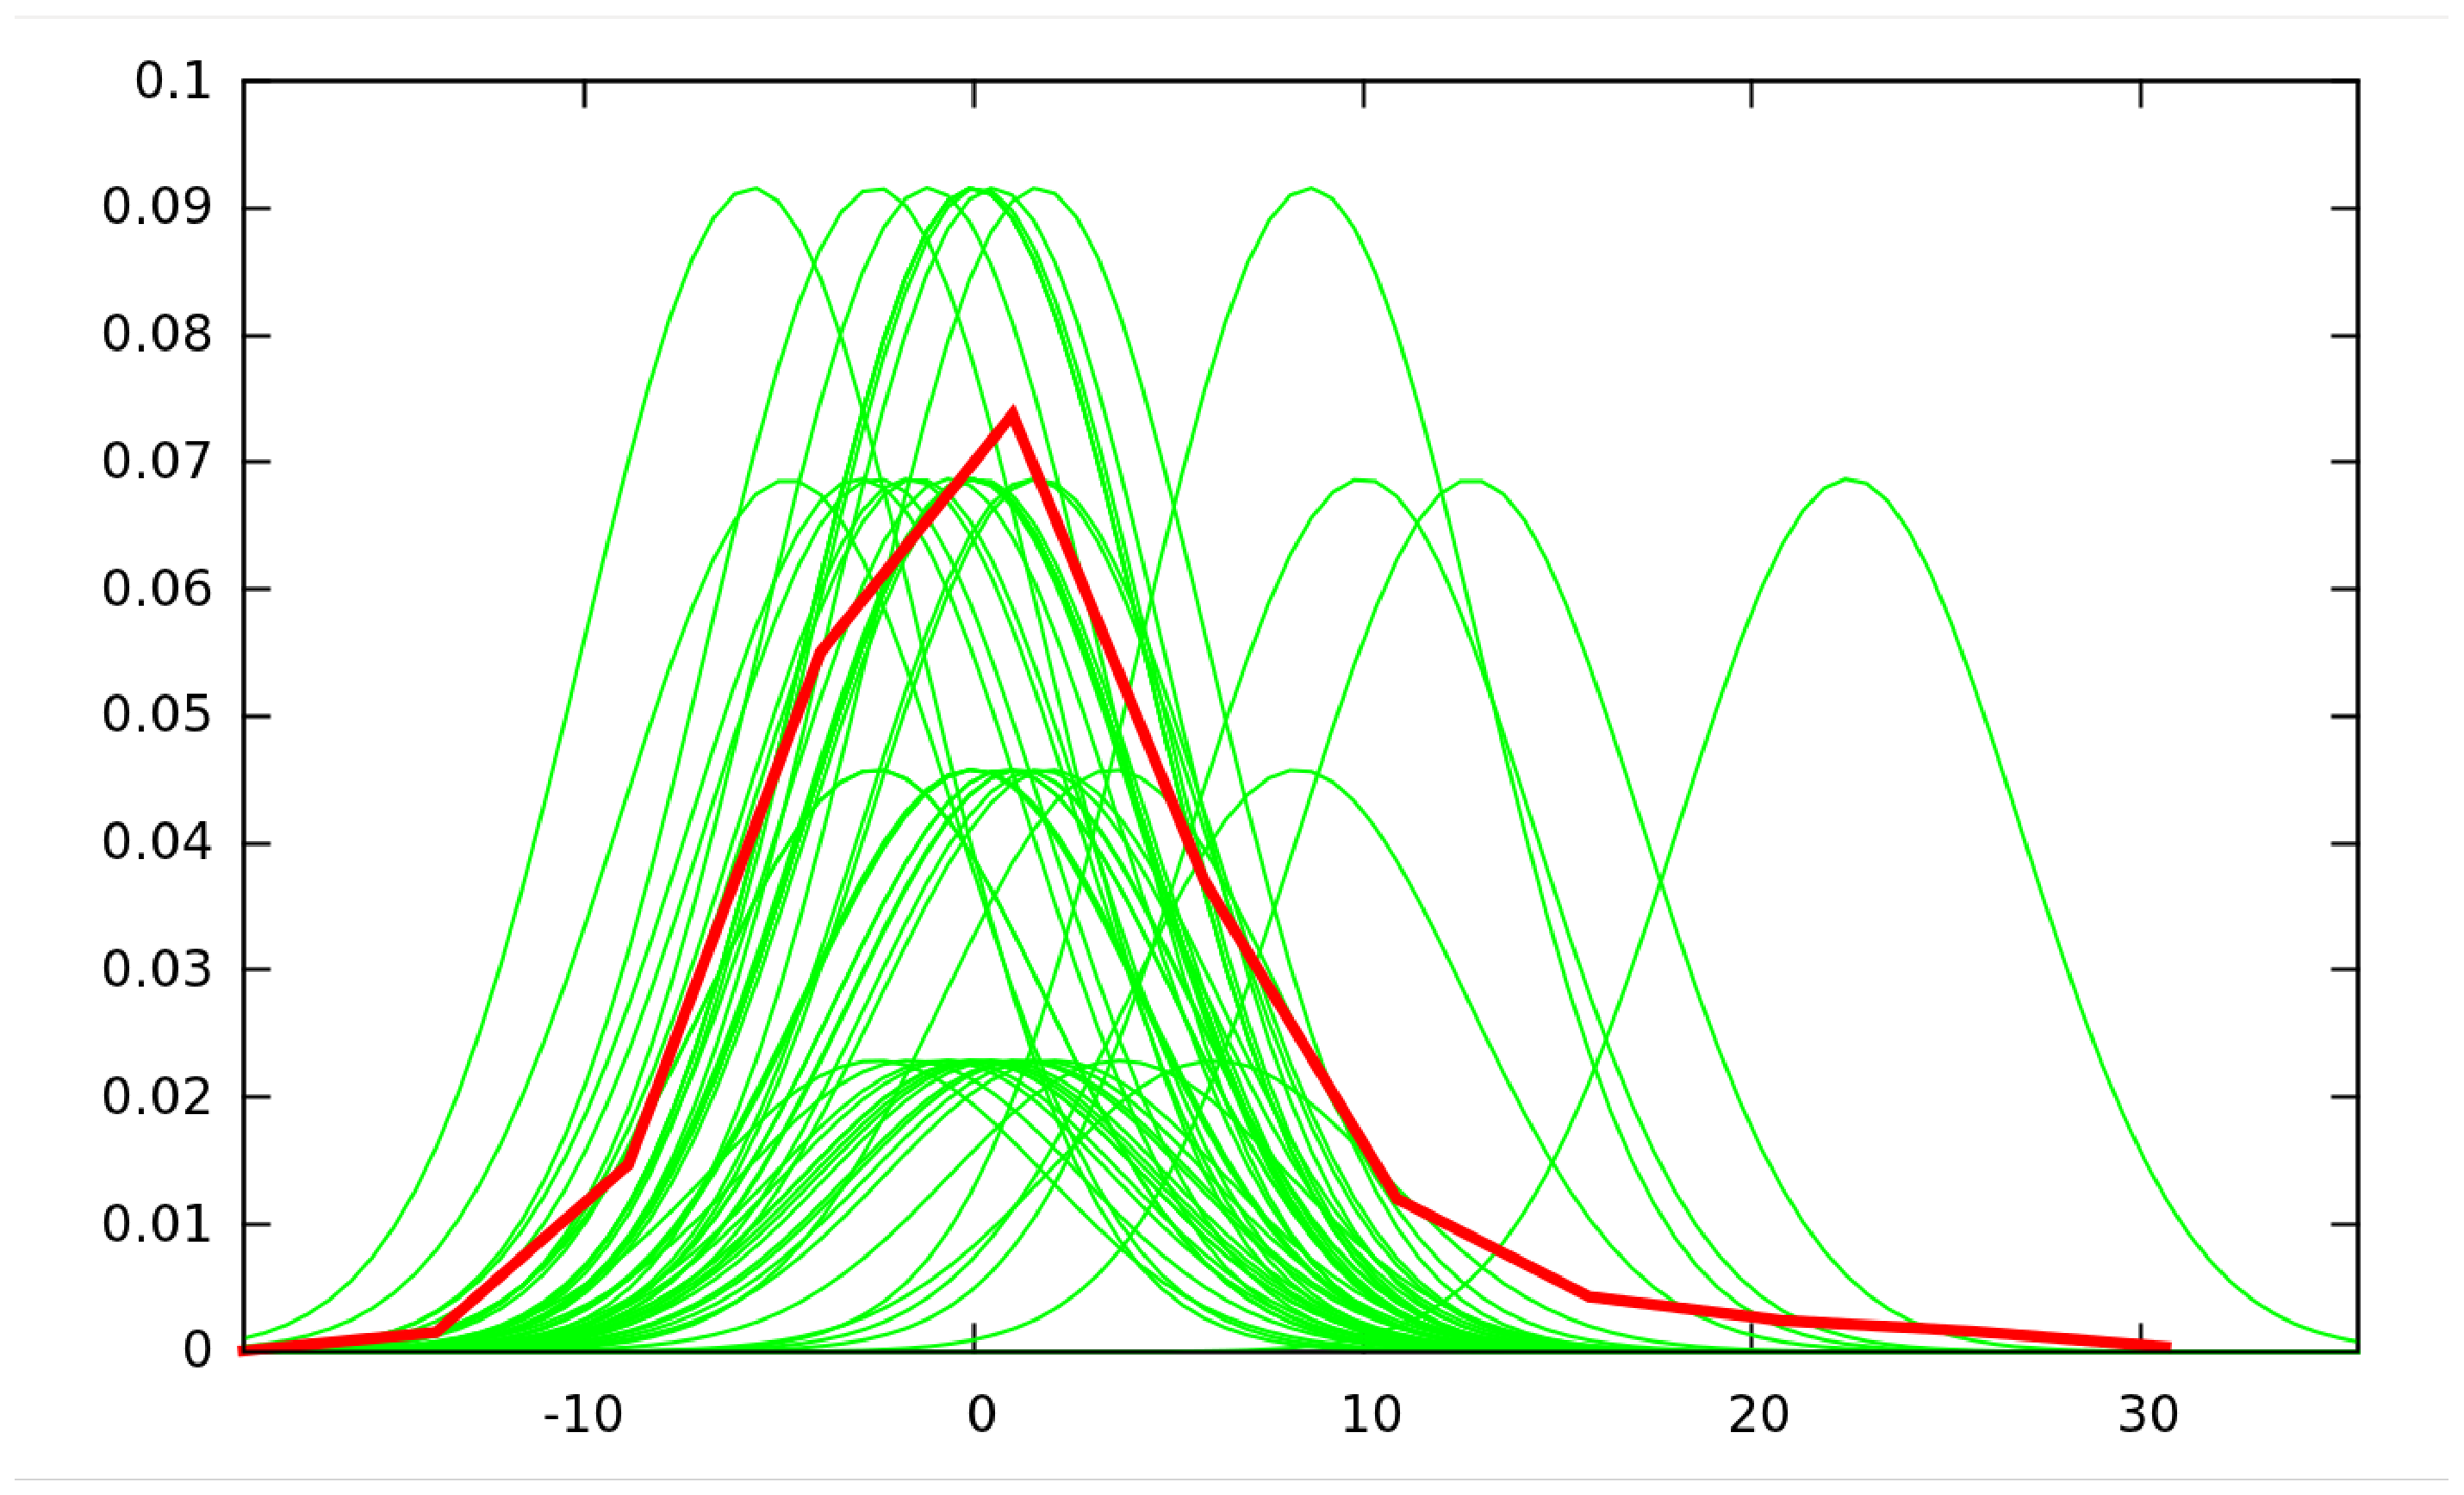
\includegraphics[width=3.0in]{figures/kde.eps}
 \caption{Example Kernel Density Estimator Construction}
 \label{fig:kde}
\end{figure}

When it is determined that historical data should be used to predict the bearing and speed change for a given segment, the appropriate bin is determined from the generated path's current location and bearing.  The latitude and longitude indicate the grid cell while the bearing indicates the bin.  The bearing and speed probability density functions from that bin are then used to generate a speed and bearing change that is consistent with the historical data.  
%To determine a bearing change, we generate a random number between 0 to 1, numerically integrate the probability density function using the trapezoidal rule until the integration reaches this number, and return the corresponding bearing change.  We compute the speed change in a similar fashion.

%This data structure and the probability density functions allow us to generate speed and bearing changes that are statistically similar to historical trends.

\section{Study}
We designed an experiment to examine how users estimate the spatial distribution of  hurricane strike probability when using our visualization versus the error cone.
Our hypothesis was that with our method, users would show a broader distribution of probabilities, more closely reflecting the uncertainty inherent in a hurricane advisory. To test this, a sequence of six historical advisories was displayed to 23 participants. The participants were all graduate students, faculty, or administrators in the School of Computing at Clemson University.  Each advisory was shown twice consecutively, once with the error cone and once with our visualization method. The order that the methods were shown was alternated between participants so that half saw the error cone first and half saw our visualization method first.  The order of the historical advisories was the same for all participants.

As show in Fig.~\ref{fig:exp}, a map of the Gulf of Mexico region was displayed, with a circle divided into eight sectors centered over the current position of the hurricane.  The sectors were aligned to the cardinal directions, and users were asked to place a set of numbered chips in the sectors to indicate their estimate of the probability that the hurricane would exit the circle in the corresponding sector. We used the distribution of  chips across all of the sectors as our measure of each participant's ability to estimate hurricane strike probability.

\begin{figure}[htb]
  \centering
  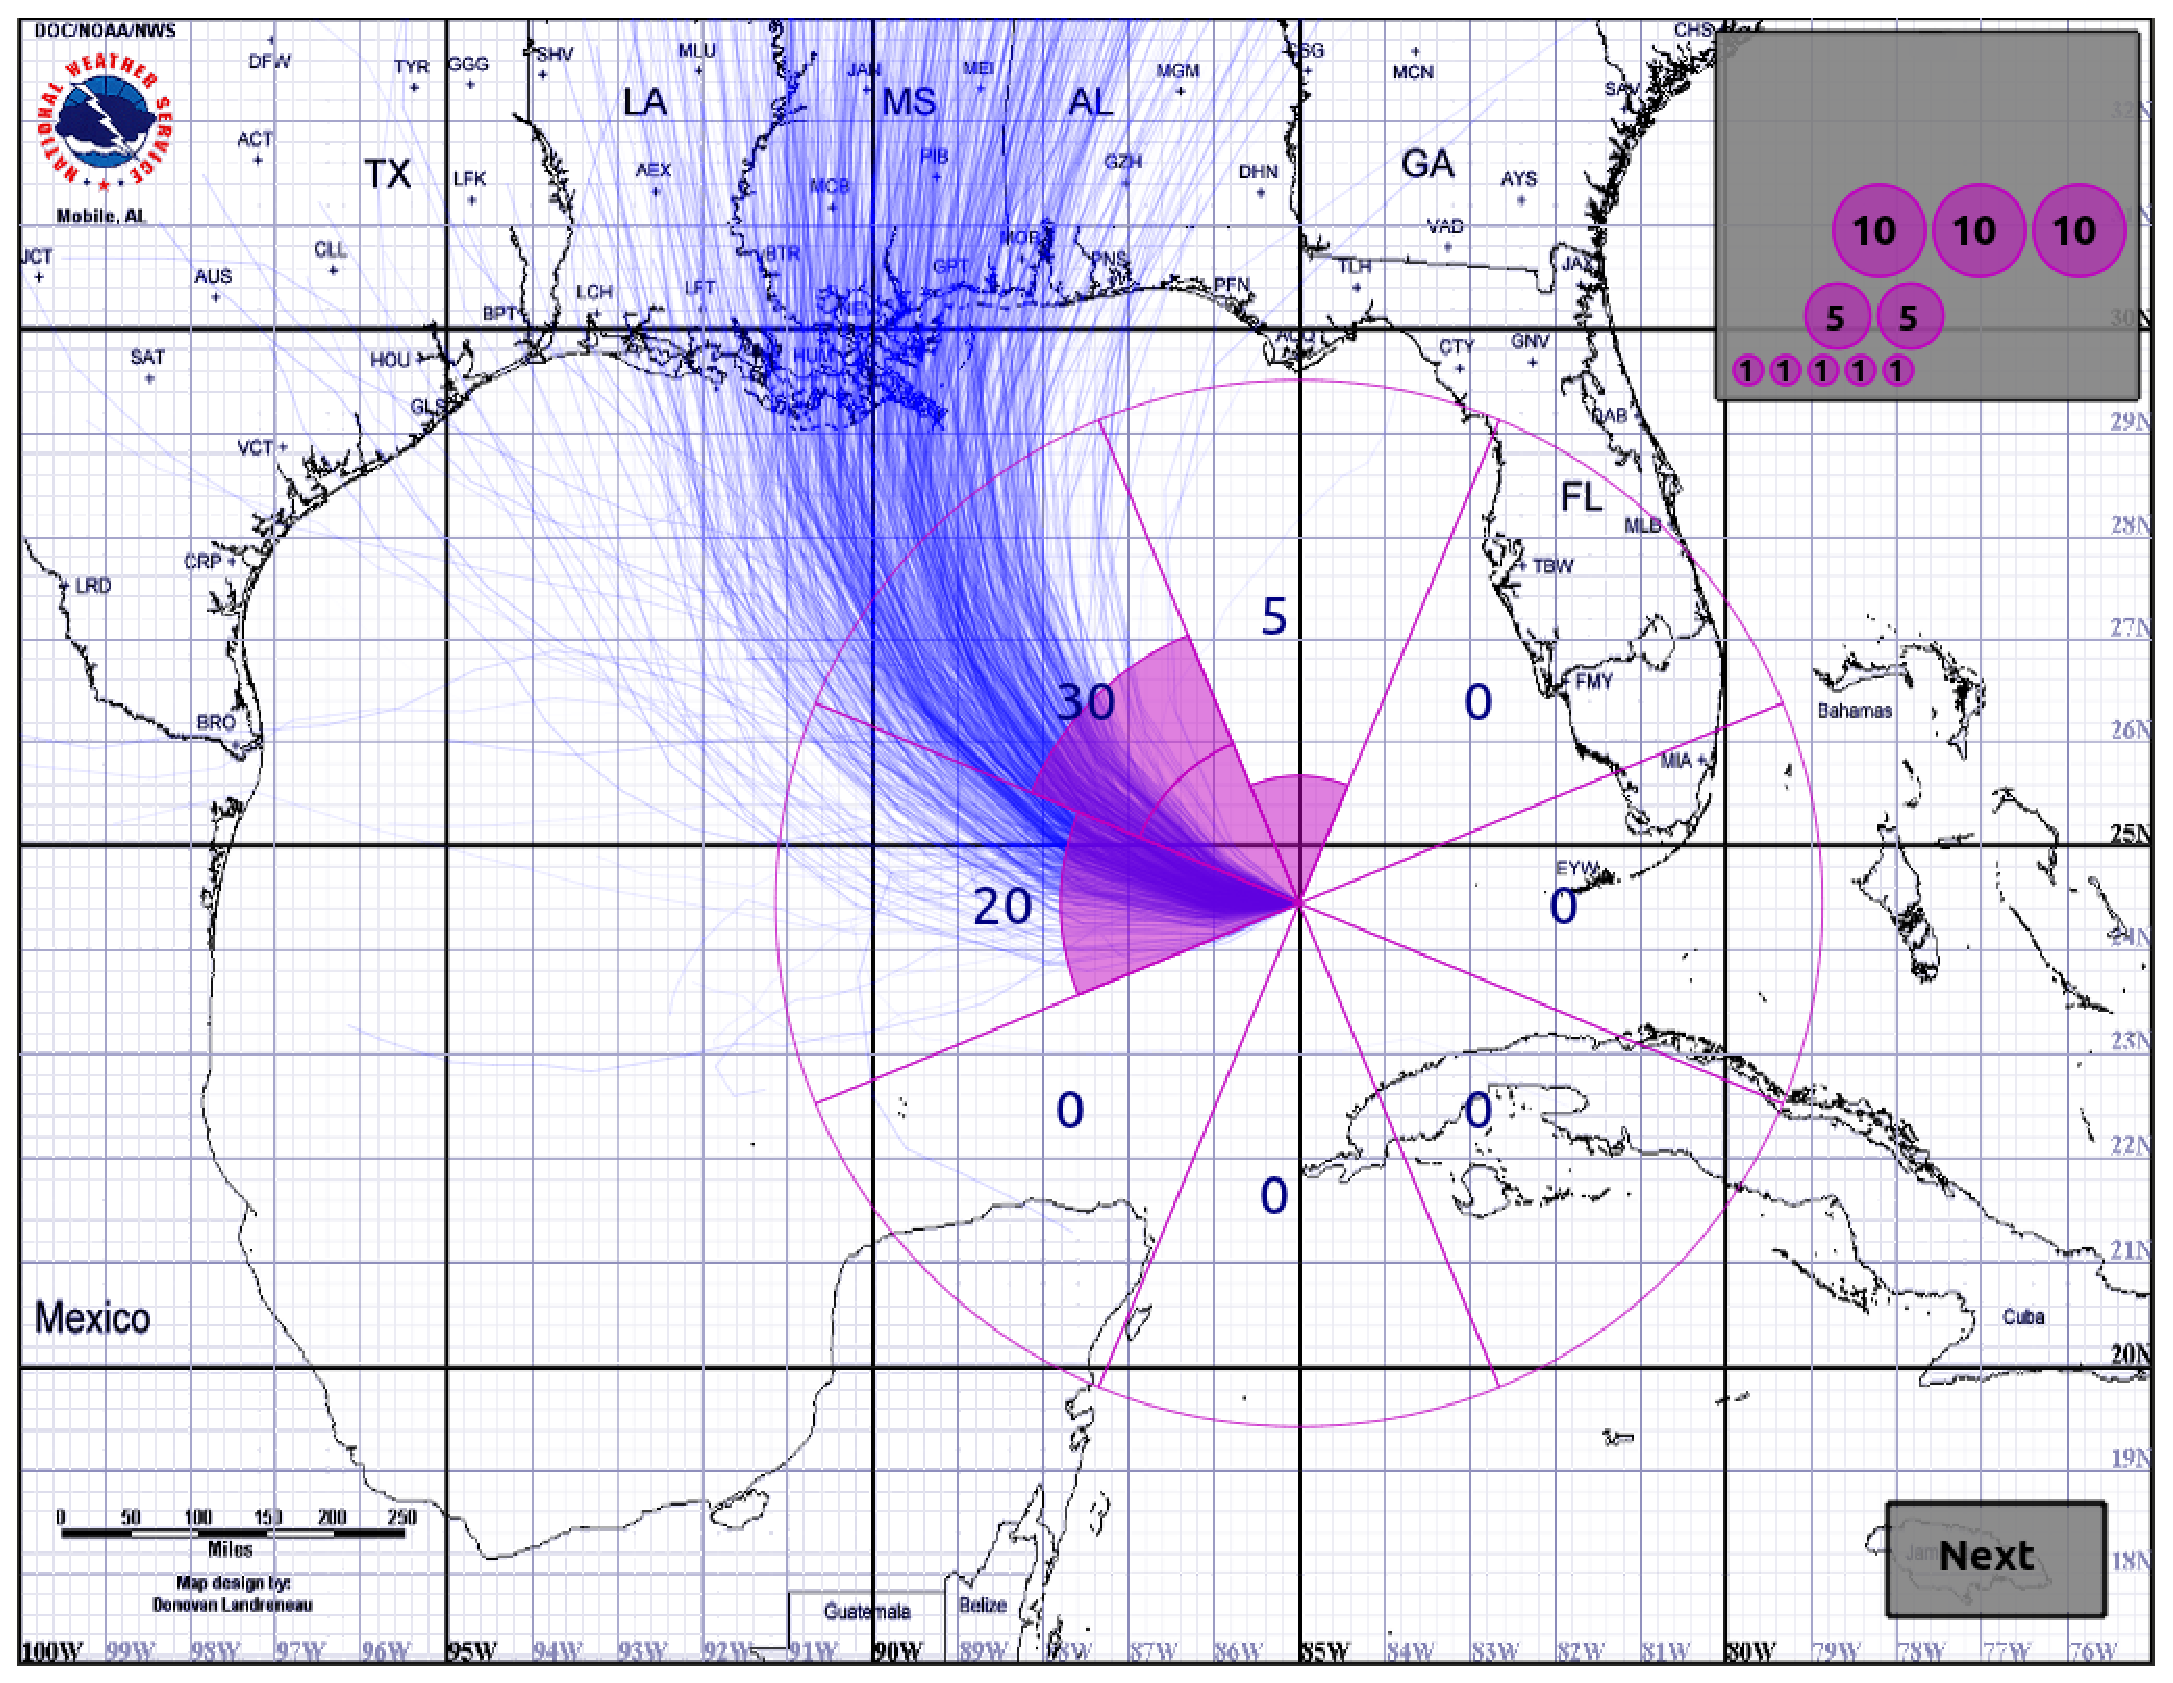
\includegraphics[width=3.0in]{figures/exp.eps}
  \caption{Interface for Our Experimental Design}
  \label{fig:exp}
\end{figure}

The chips had values ranging from 1 to 20. There were two 20's, four 10's, three 5's, and five 1's for a cumulative value of 100. The interface assured that each chip was assigned to exactly one sector. To advance from one advisory to another, all of the chips had to be assigned.

After completing the study, each participant was also asked, on a paper and pencil questionnaire, to rate which visualization method they preferred, on a scale of 1 to 5, with a 1 indicating that they strongly preferred our method, and a 5 indicating that they strongly preferred the error cone. They were also asked for open ended comments on the study.


\section{Results}

Fig.~\ref{fig:6cases_comp} shows each of the six cases presented to the experiment participants, in their order of presentation, with the top
row of each case showing the error cone view, and the bottom row showing our method. These examples were taken from
actual  advisories, from the National Hurricane Center online archive \cite{NHC:2011:ADV}. They were chosen to represent a number of
distinct predicted paths, all occuring in the Gulf of Mexico region. The most famous is Case 5, which is an advisory for Hurricane Katrina.

\begin{figure*}[pt]
 \centering
 
 \hbox{
   \parbox[b]{2in}{
       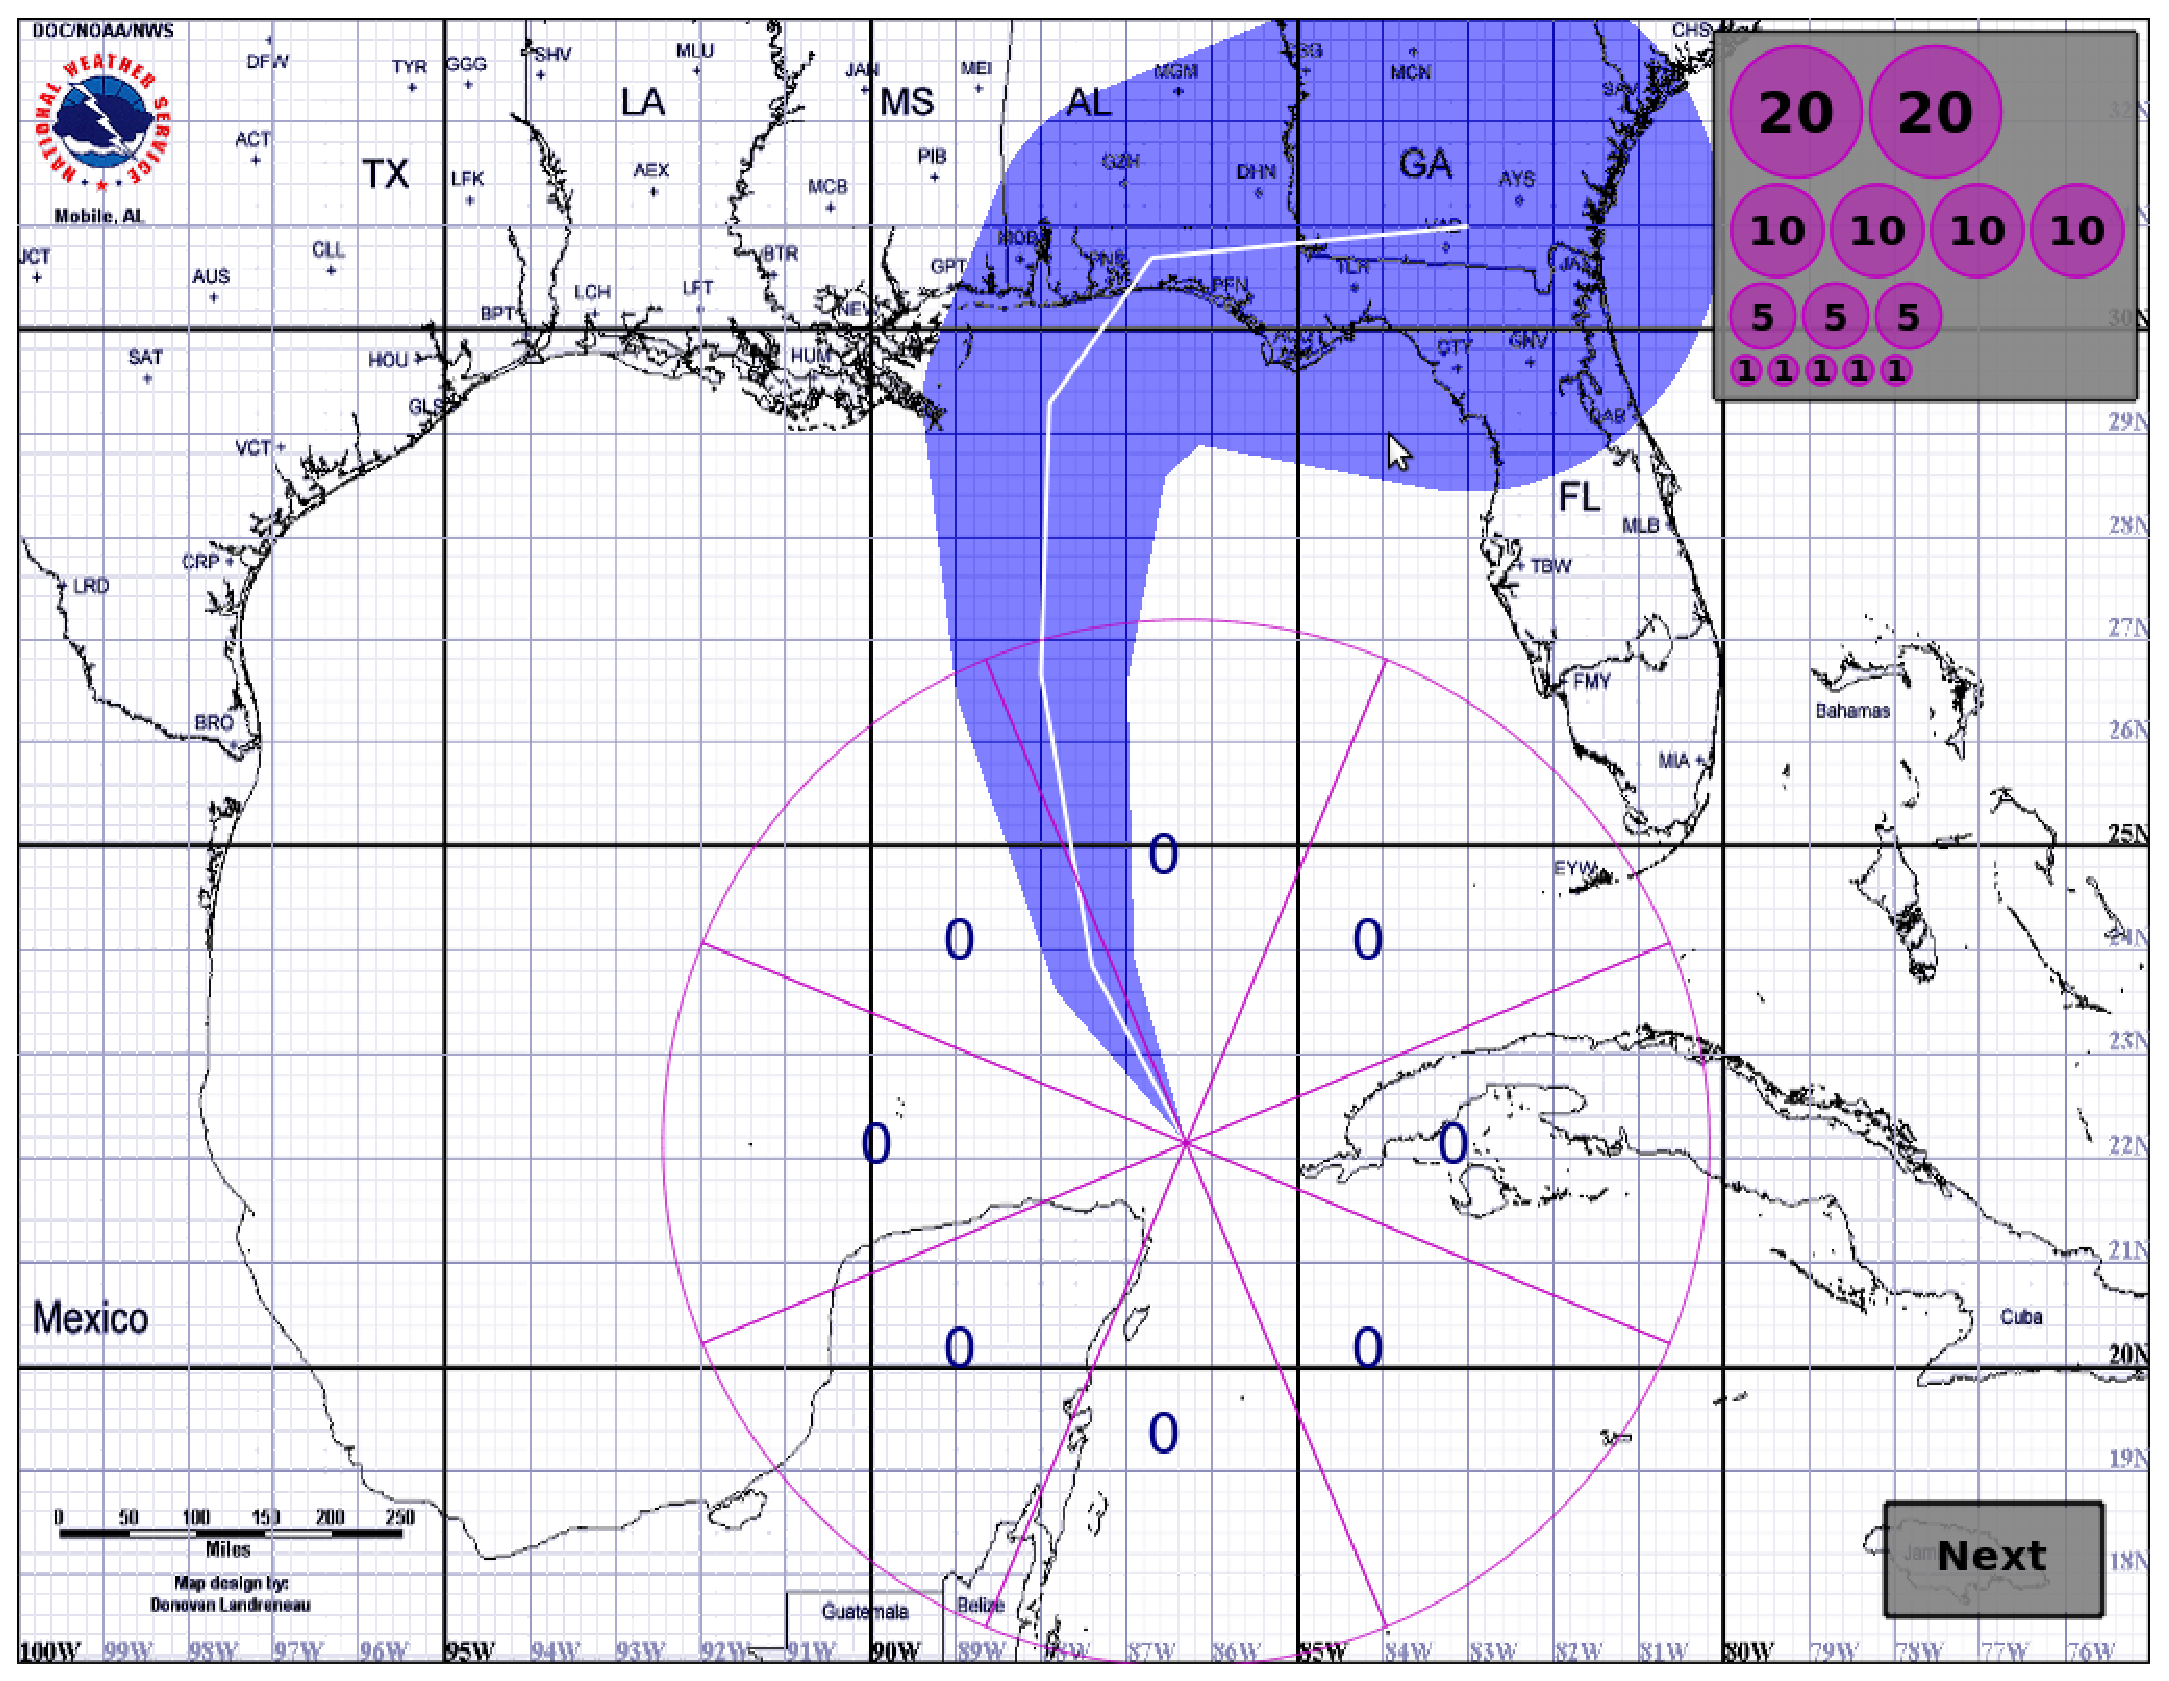
\includegraphics[width=2.0in]{figures/case_1_1.eps}
       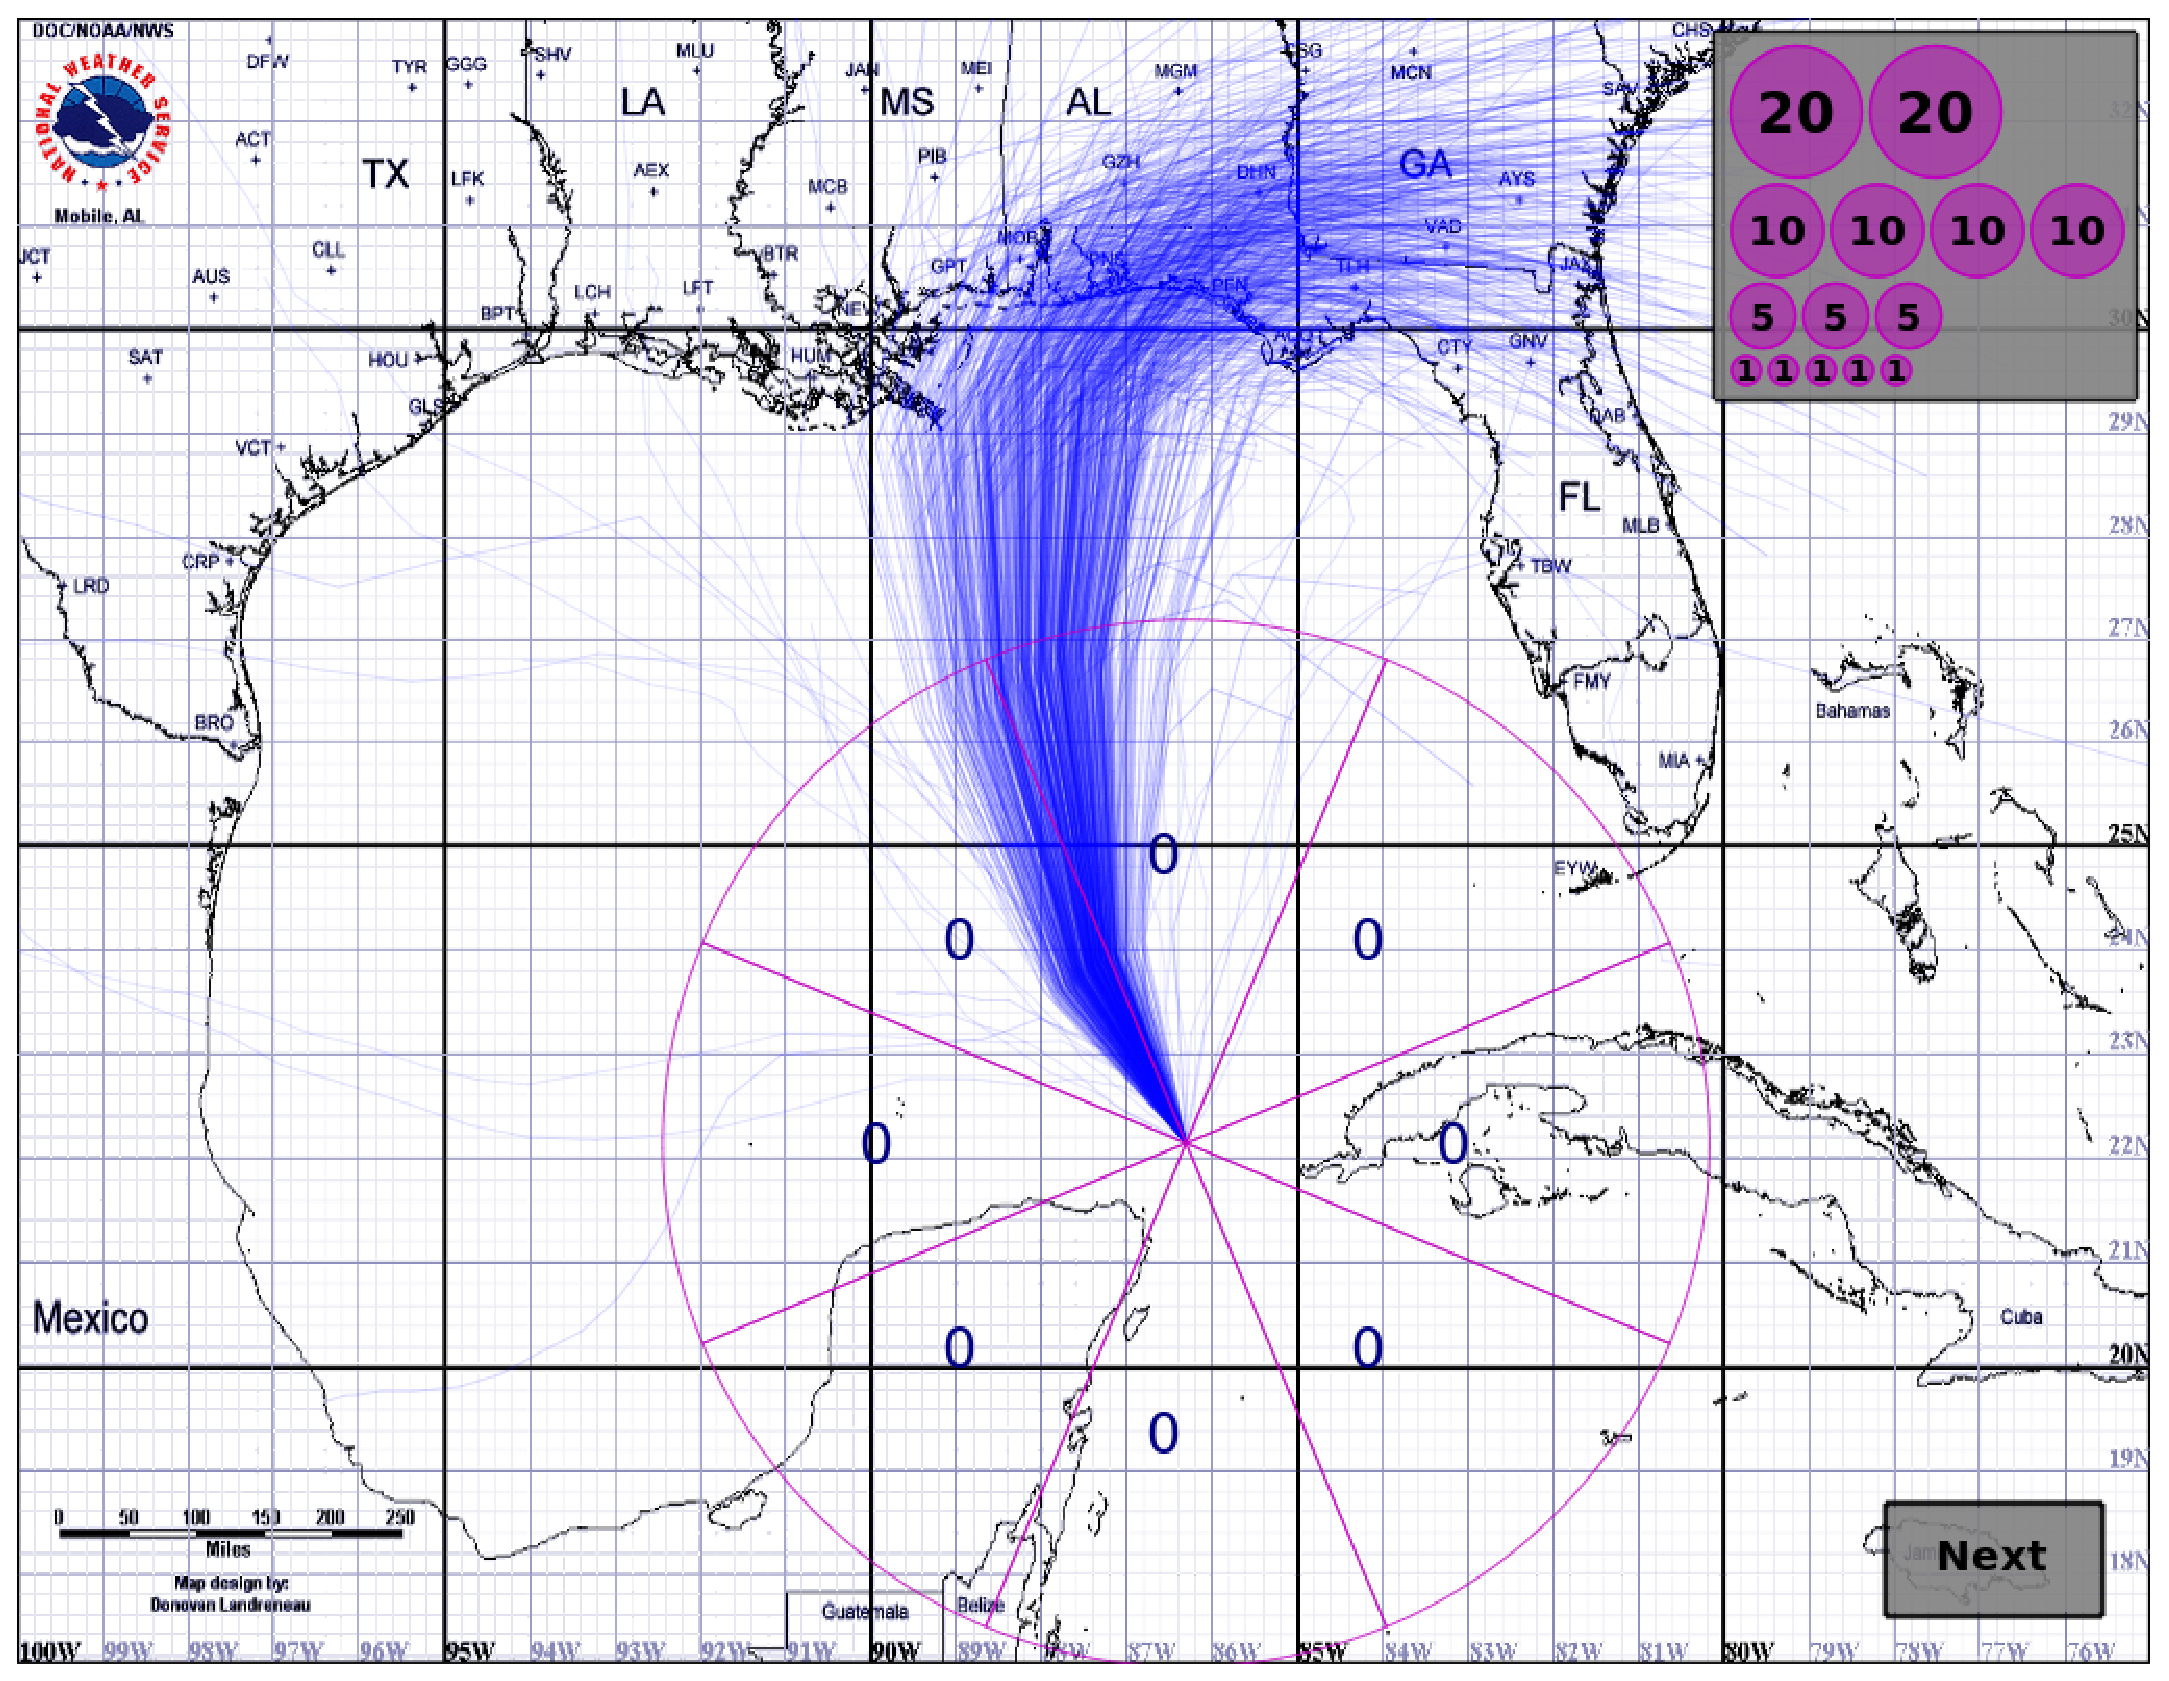
\includegraphics[width=2.0in]{figures/case_1_0.eps}
       \centerline{\small Case 1}}
       \hspace{1em}
   \parbox[b]{2in}{
       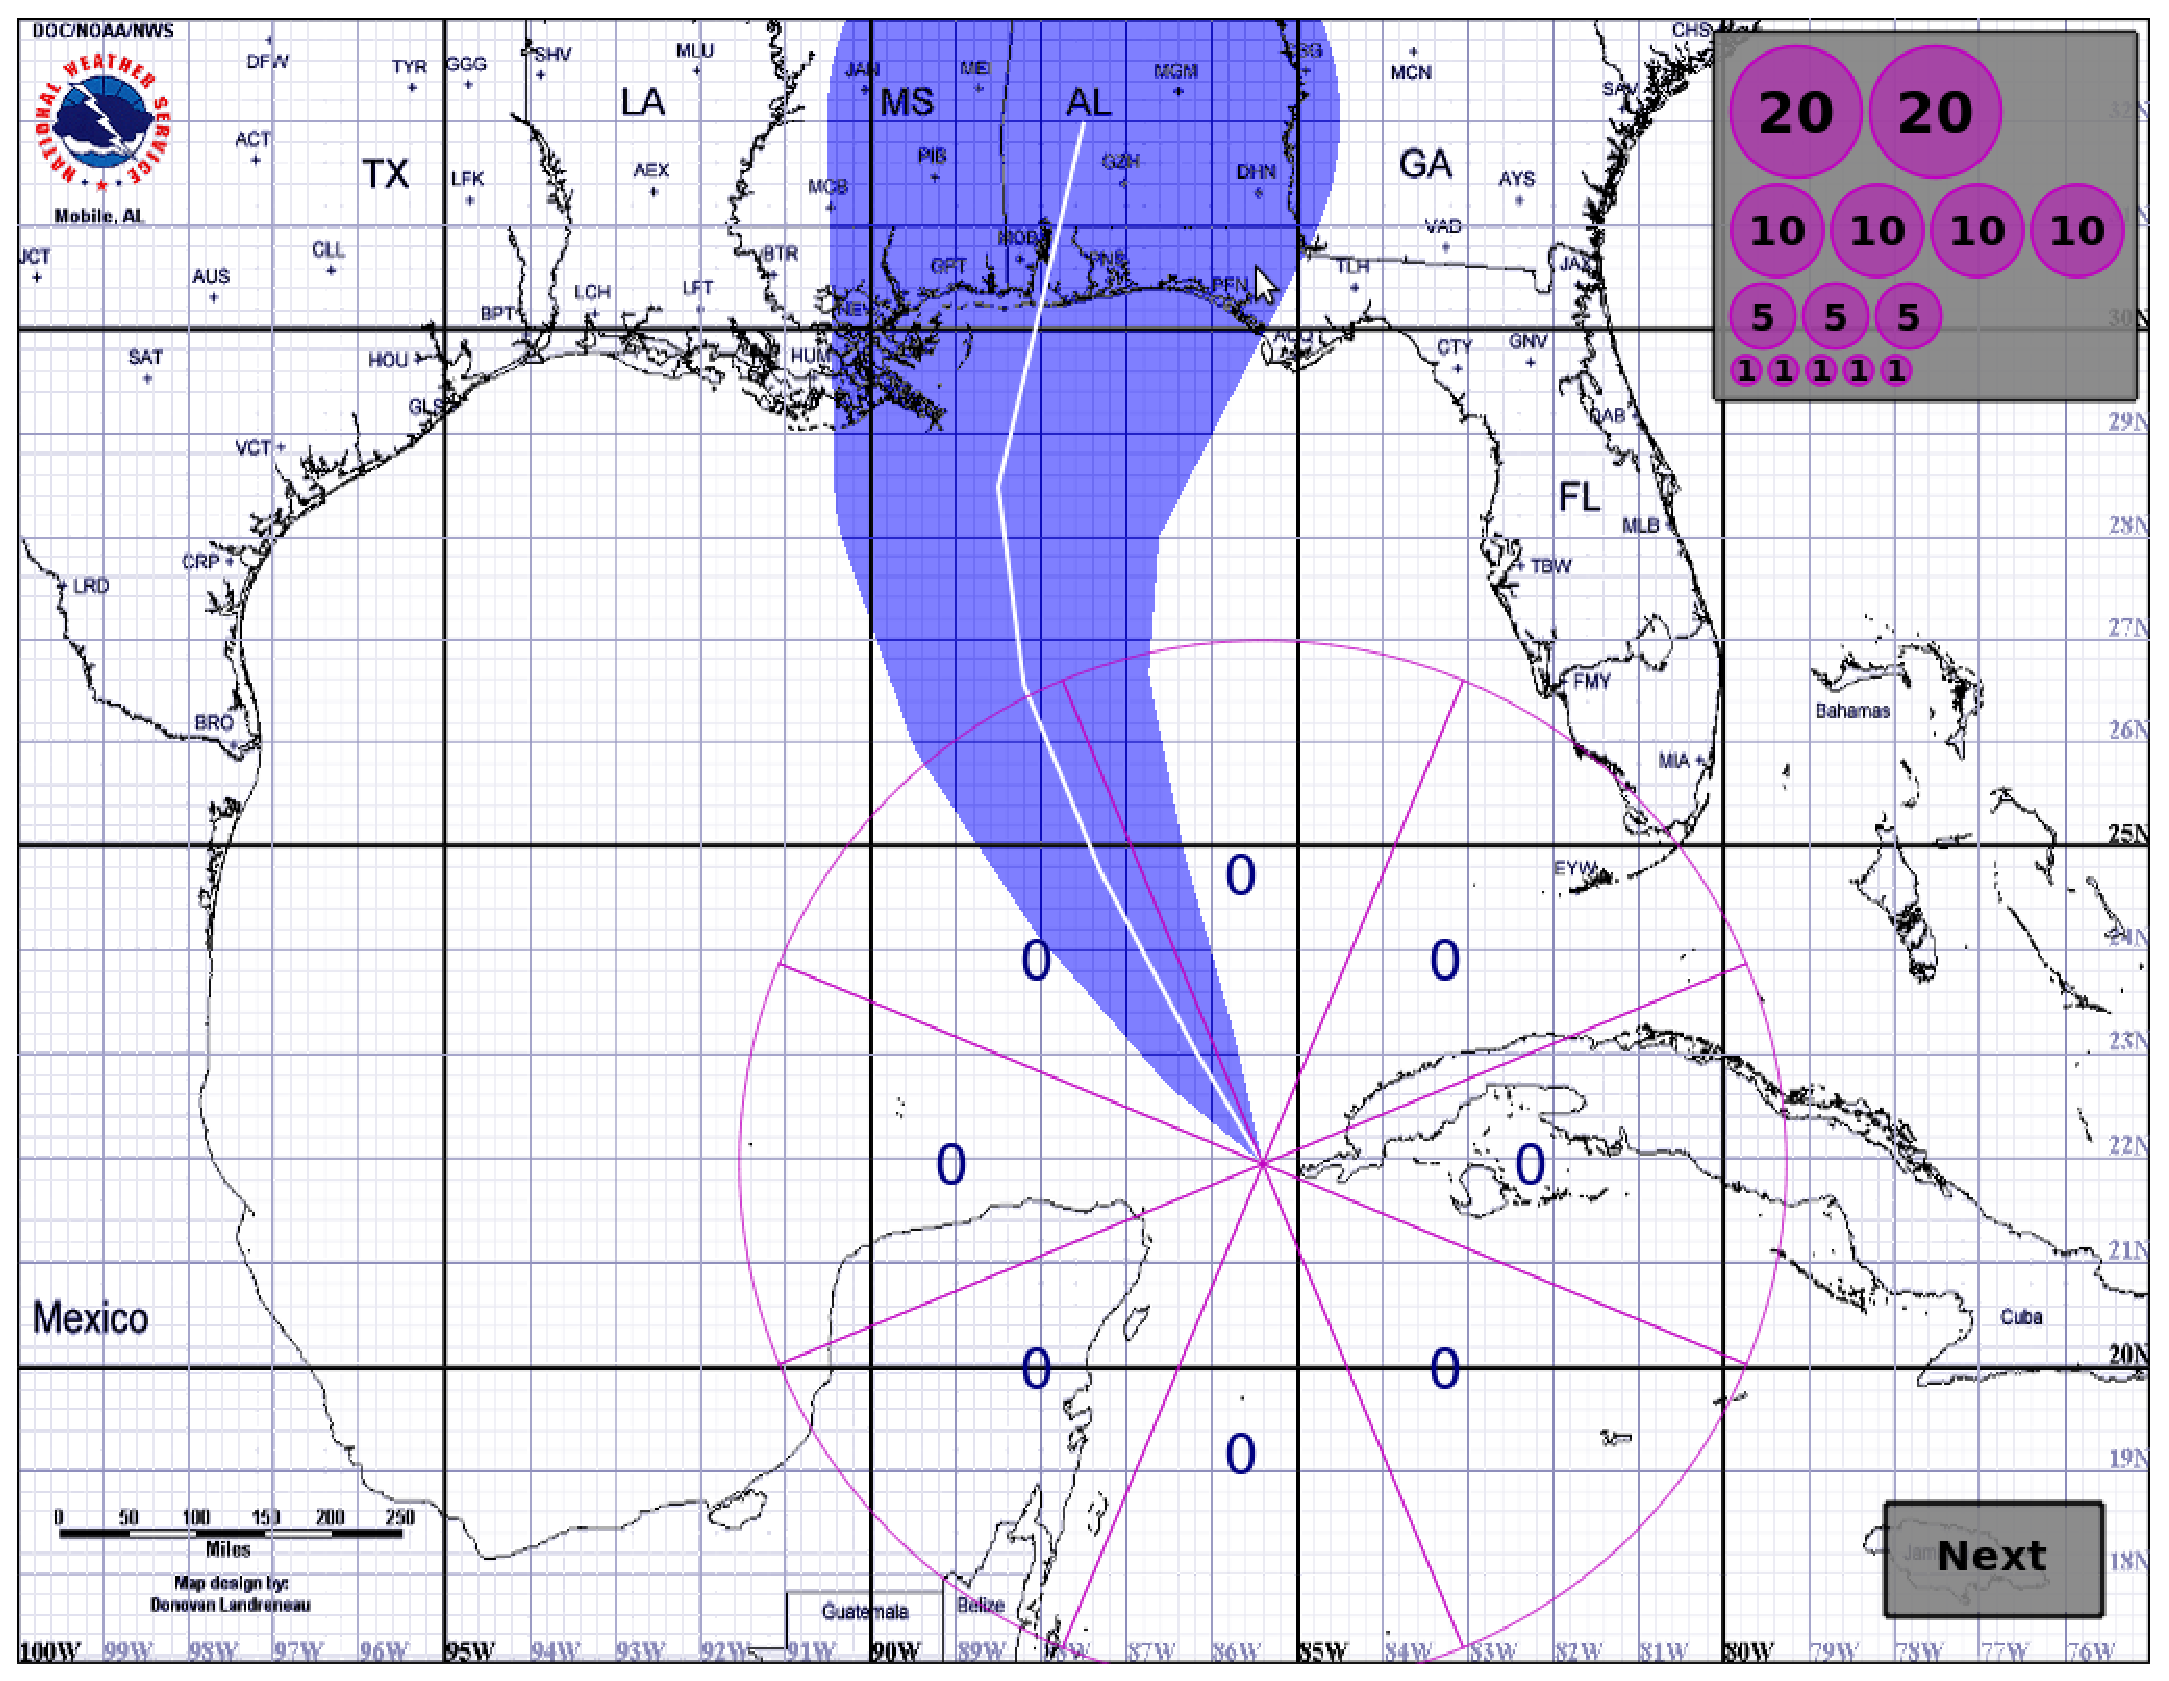
\includegraphics[width=2.0in]{figures/case_2_1.eps}
       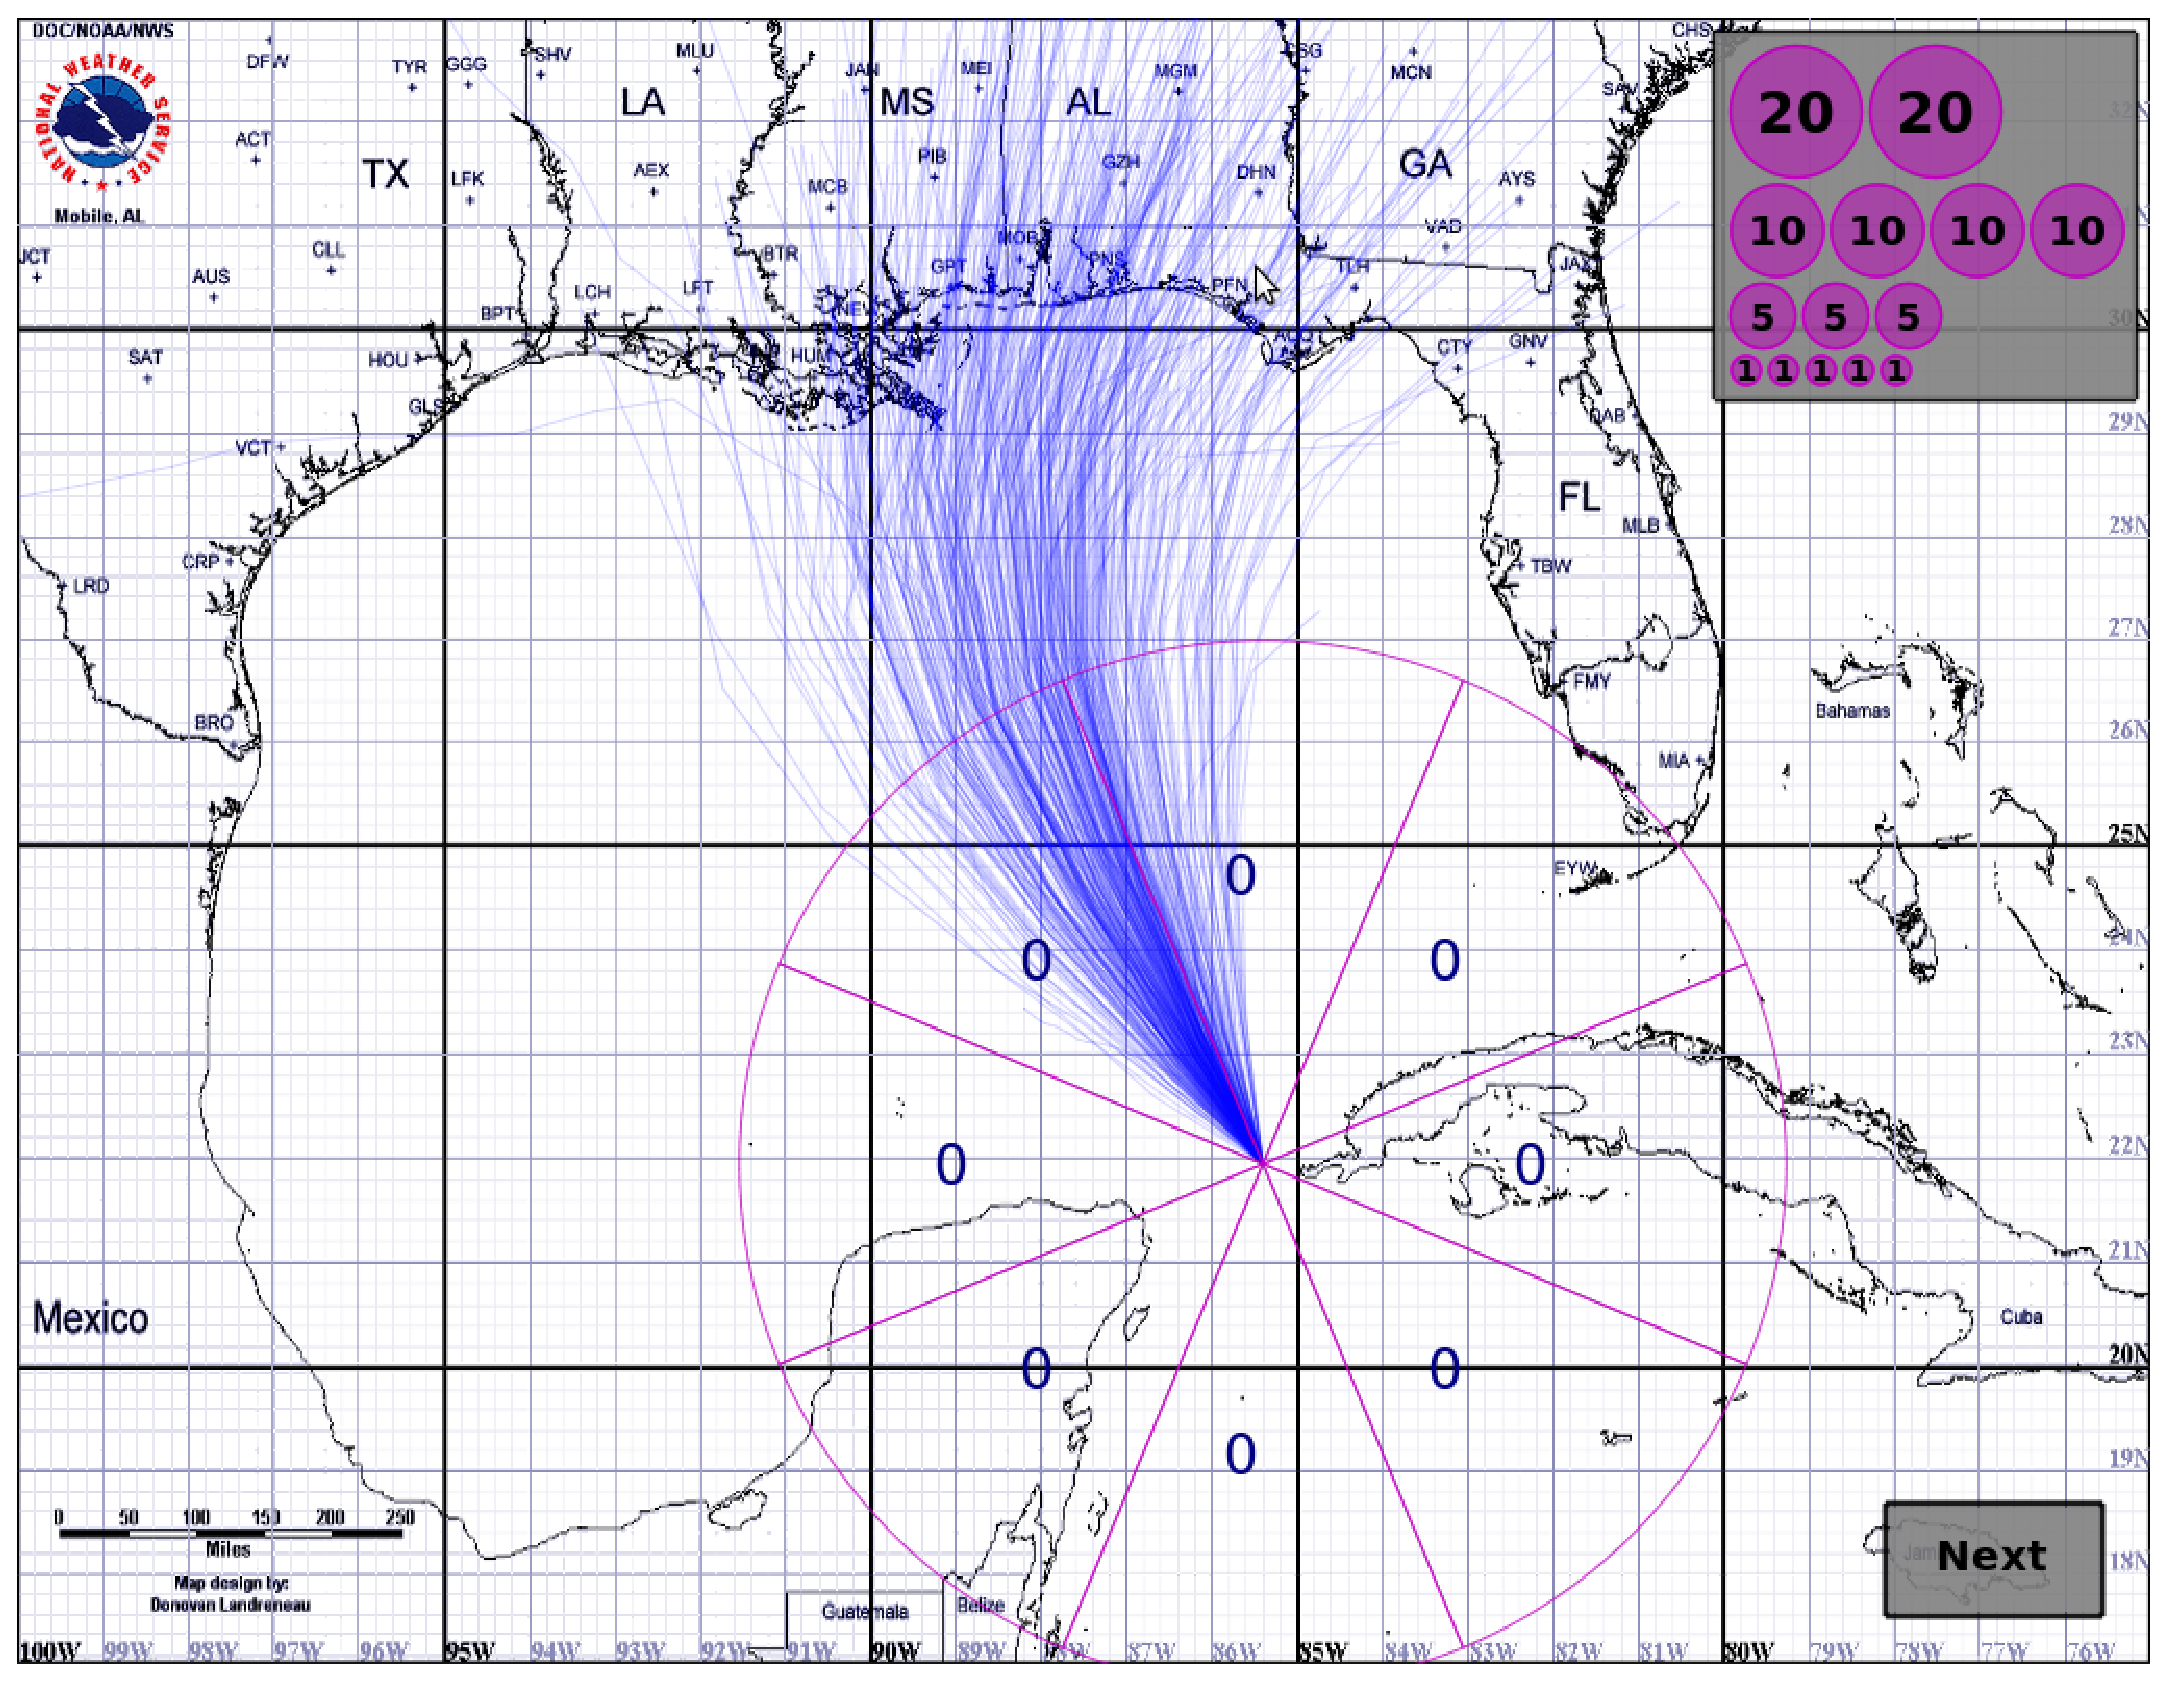
\includegraphics[width=2.0in]{figures/case_2_0.eps}
       \centerline{\small Case 2}}
       \hspace{1em}
    \parbox[b]{2in}{
       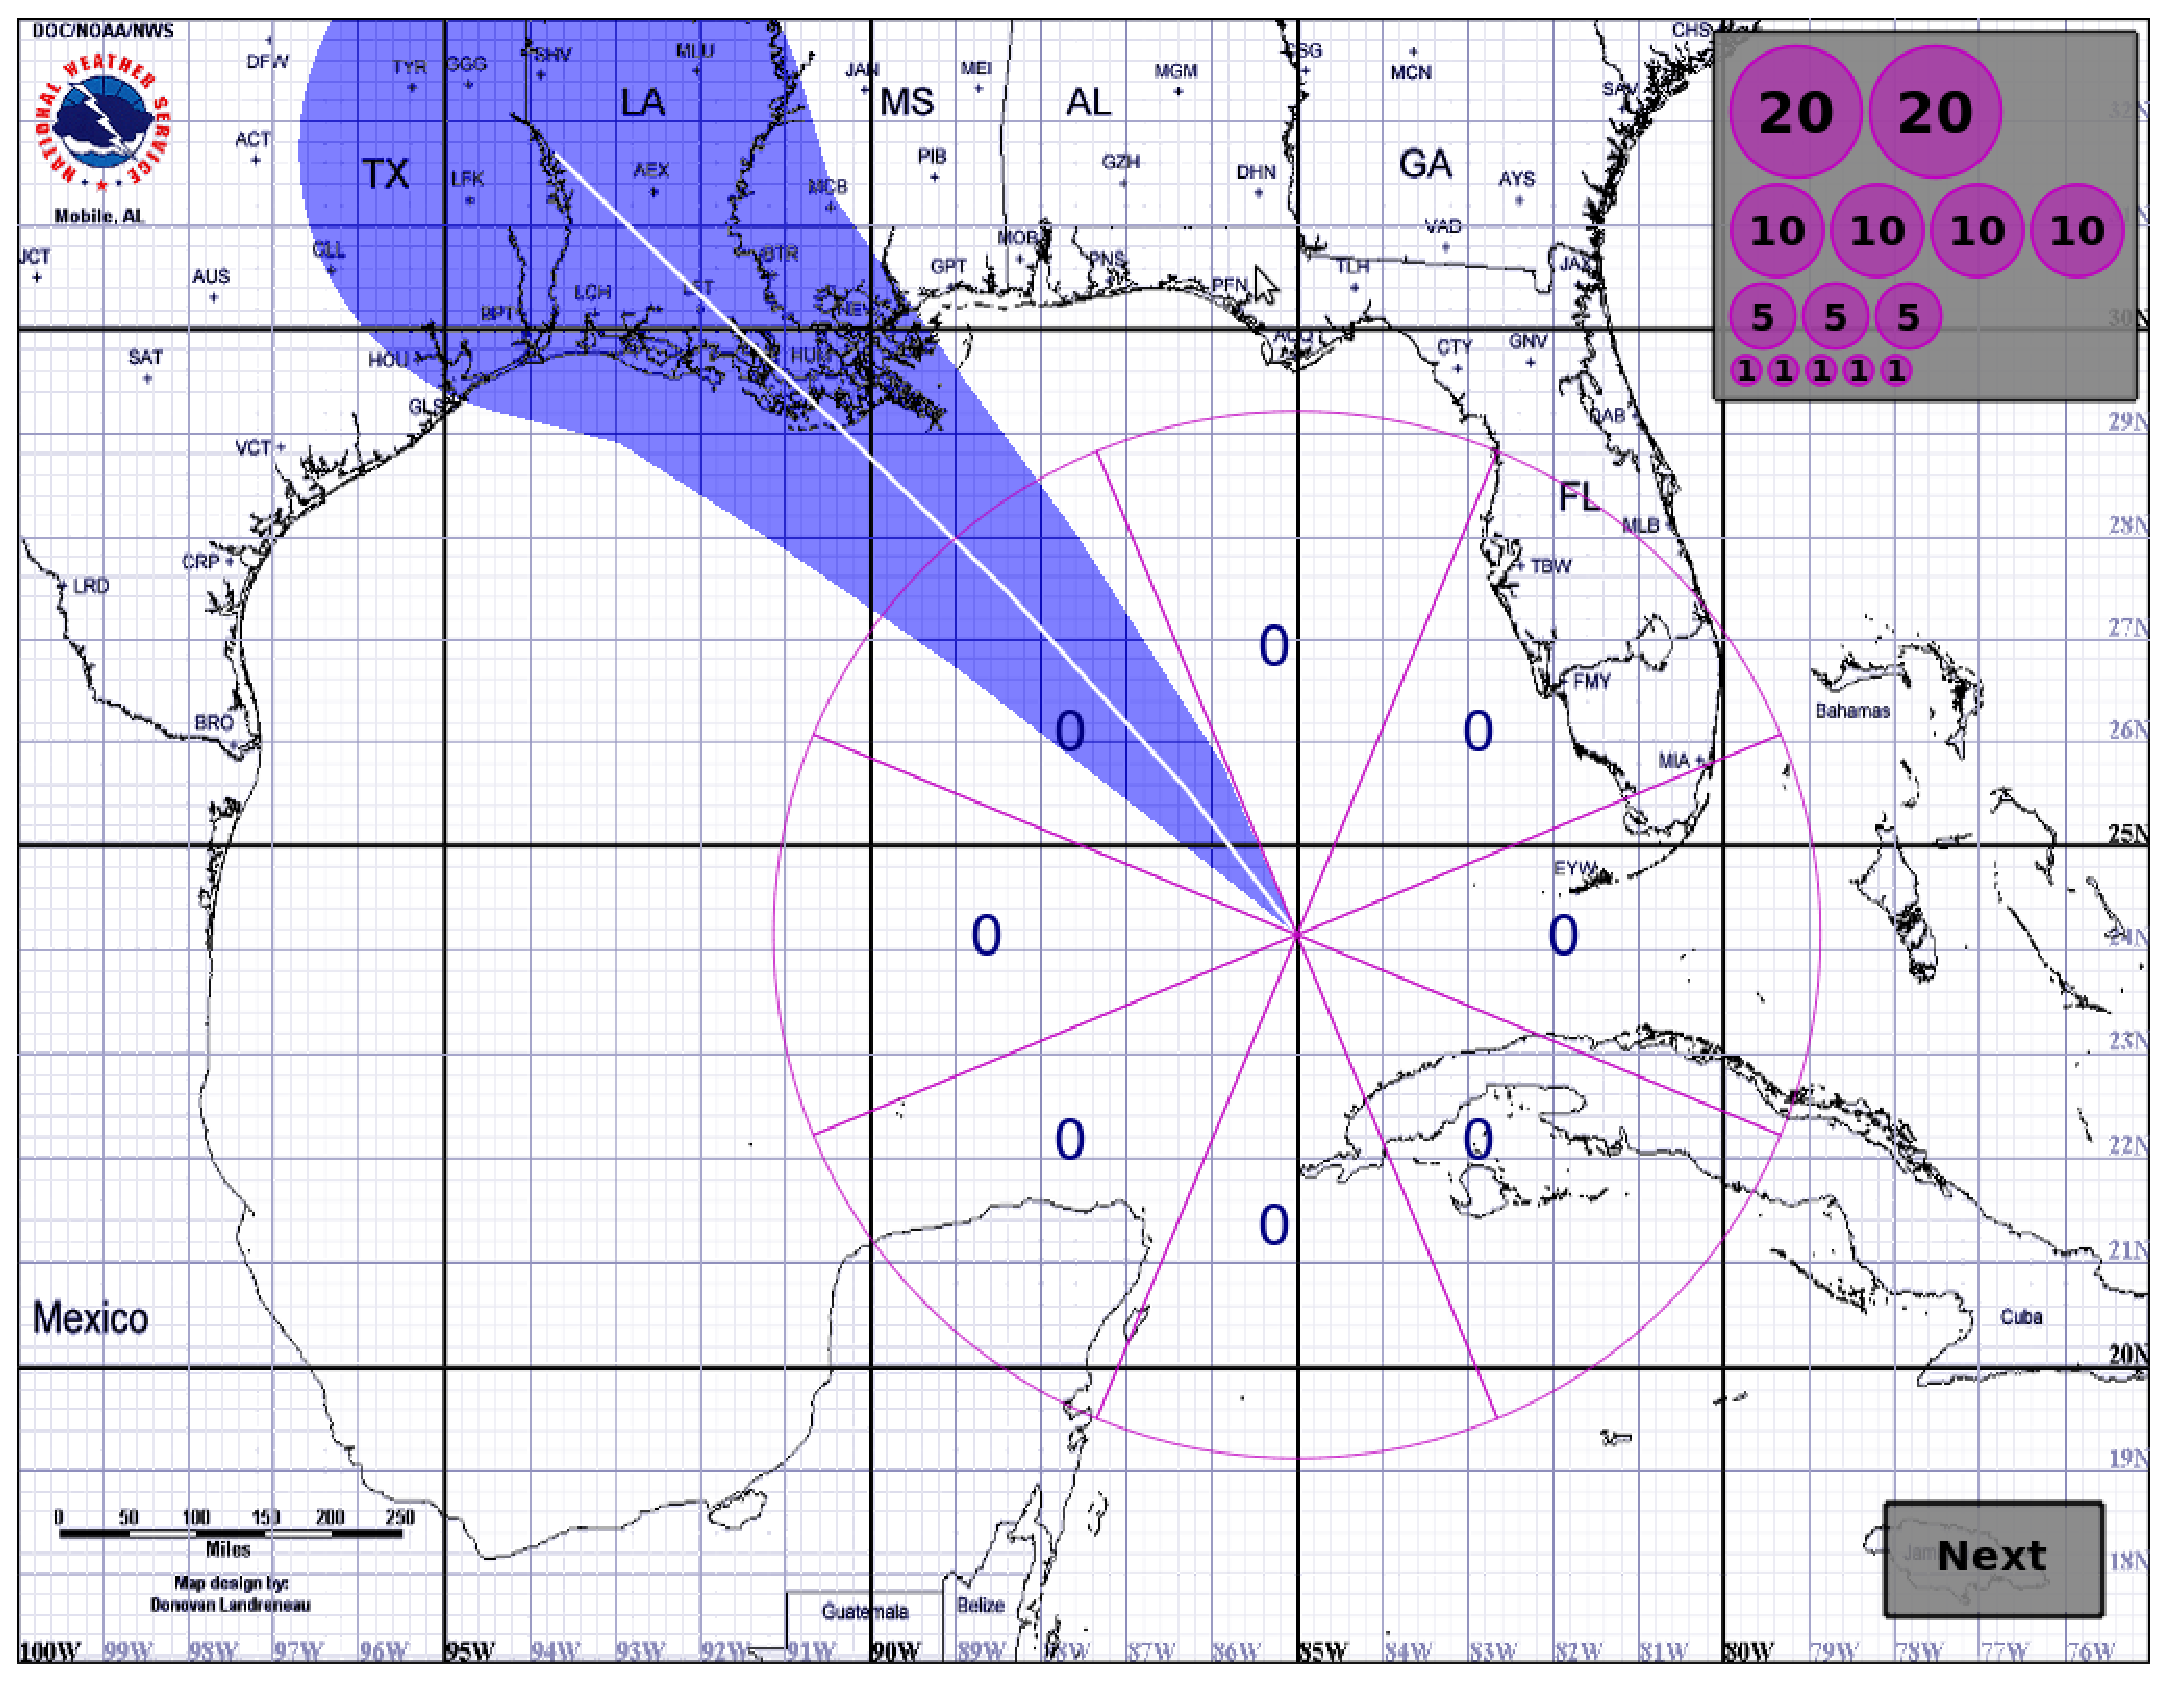
\includegraphics[width=2.0in]{figures/case_3_1.eps}
       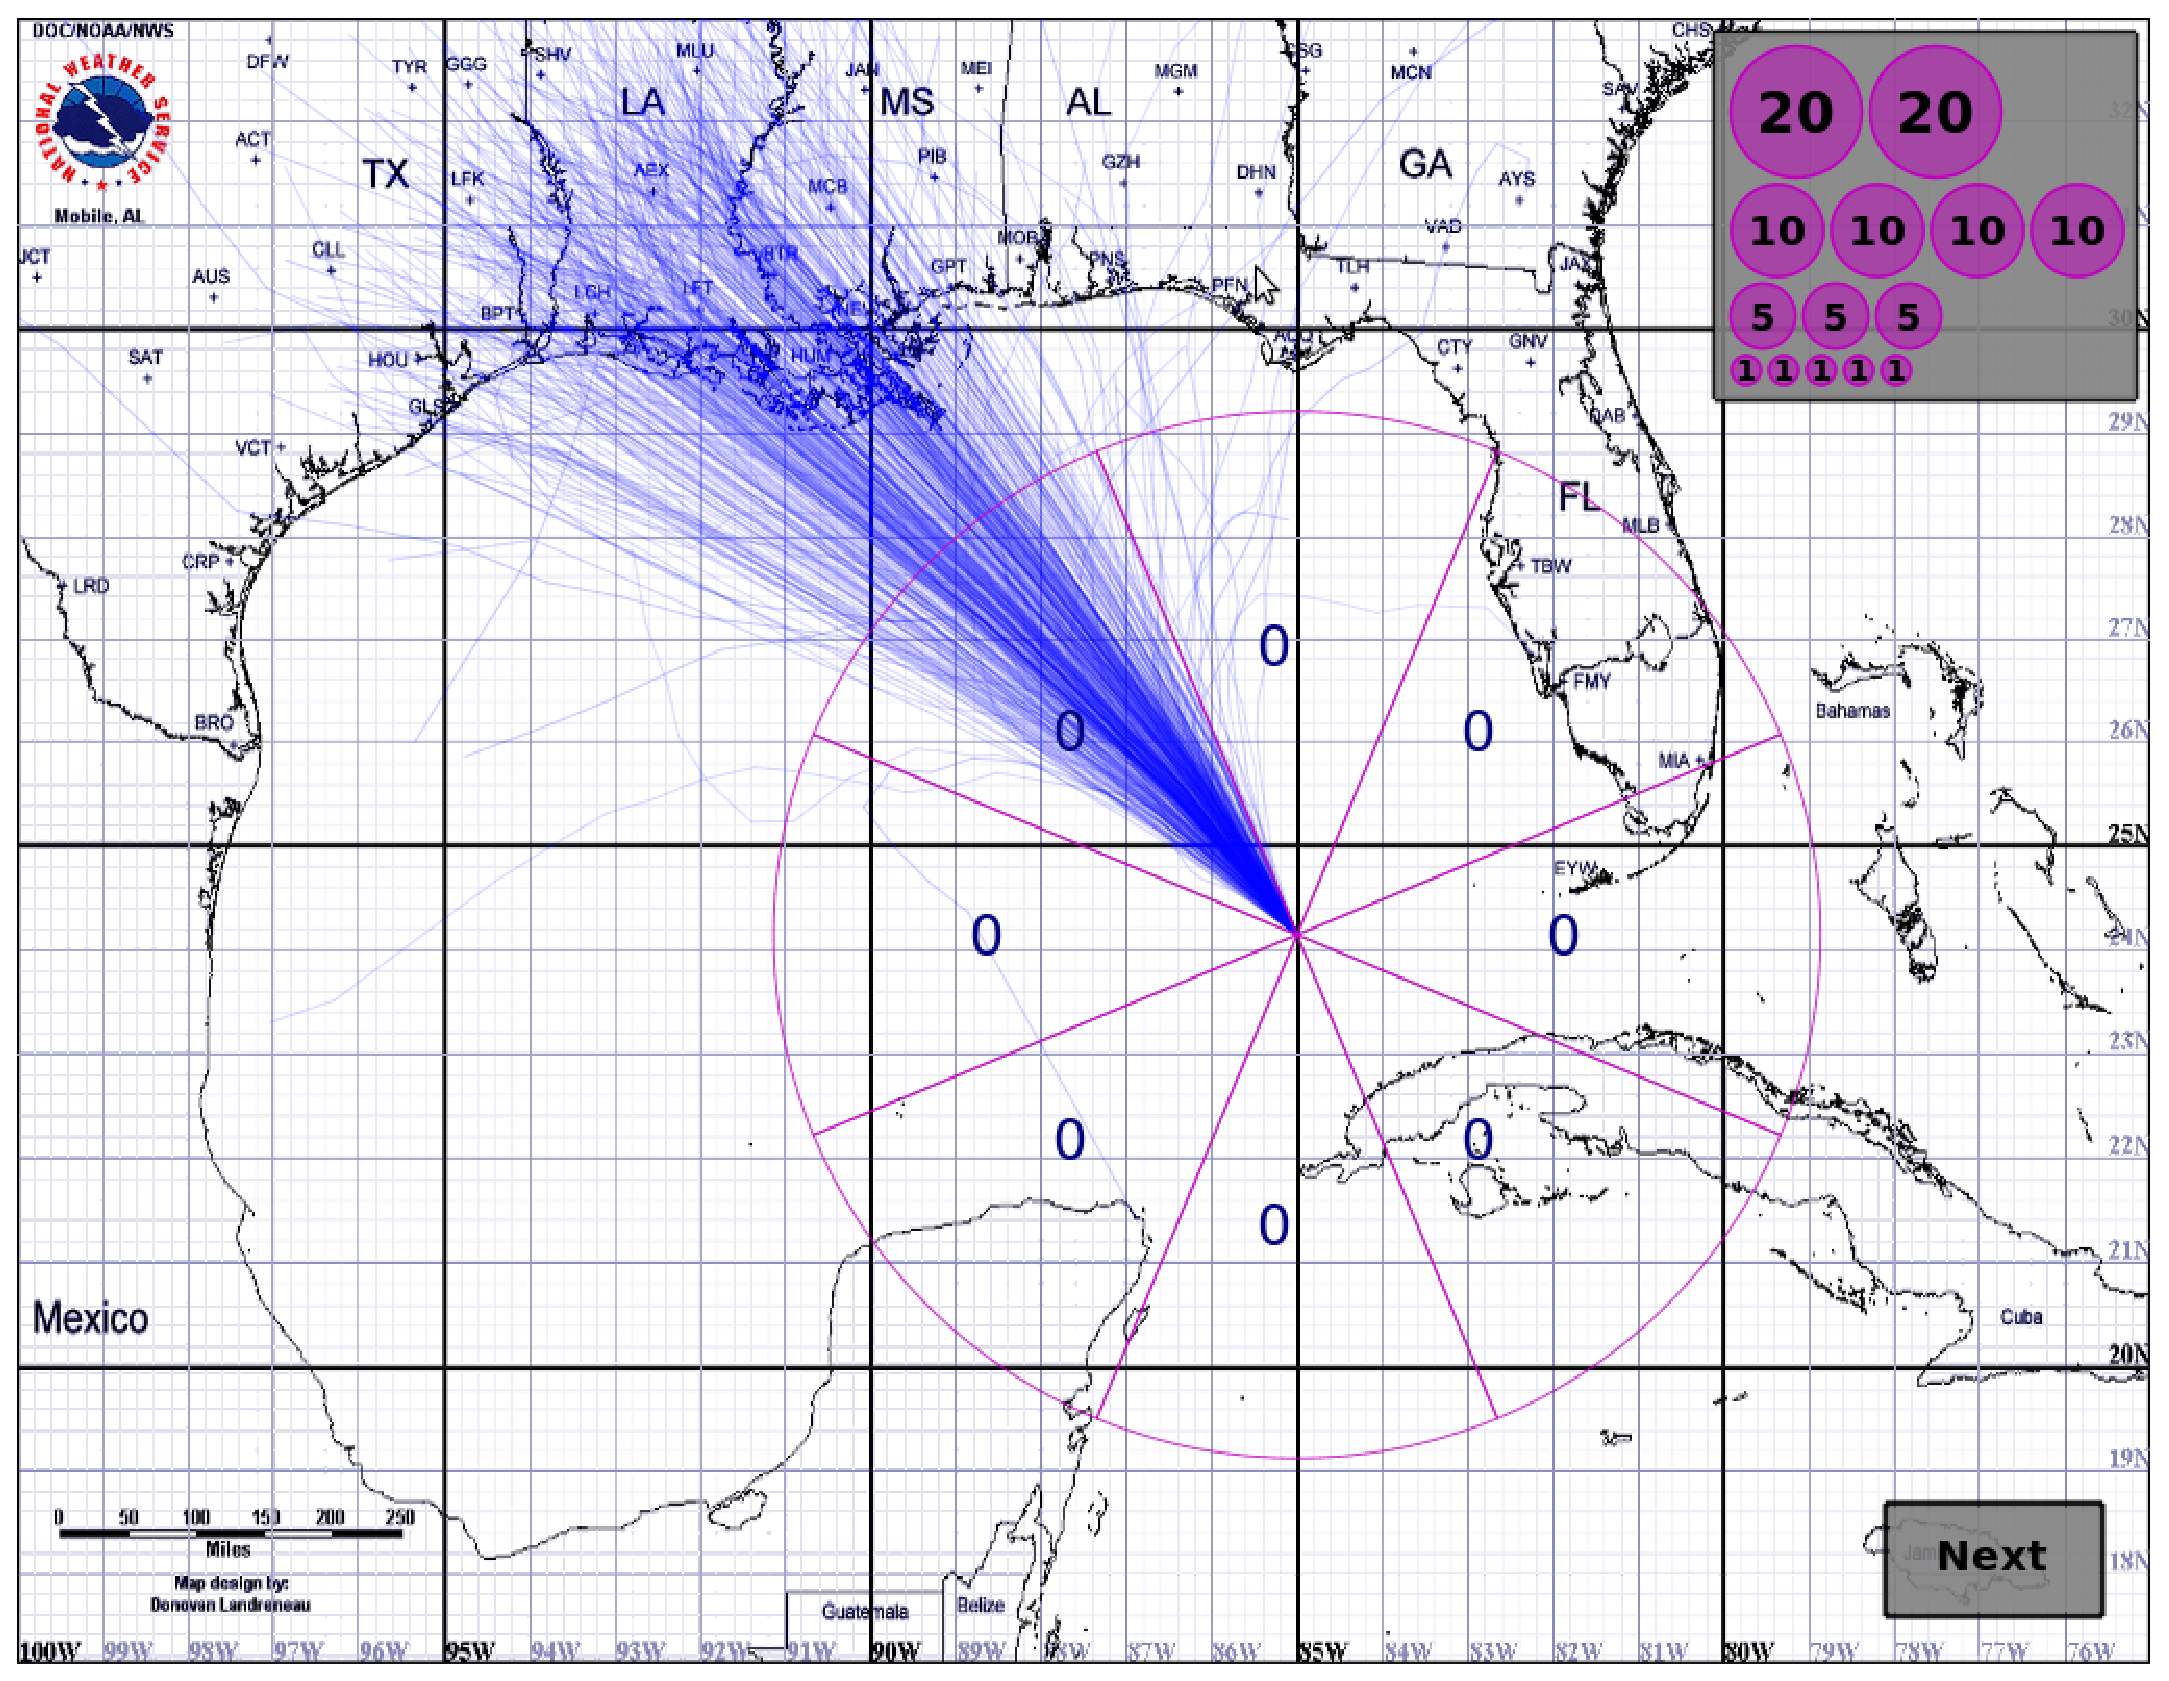
\includegraphics[width=2.0in]{figures/case_3_0.eps}
       \centerline{\small Case 3}}
   }
 \vspace{10pt}
 \hbox{
    \parbox[b]{2in}{
       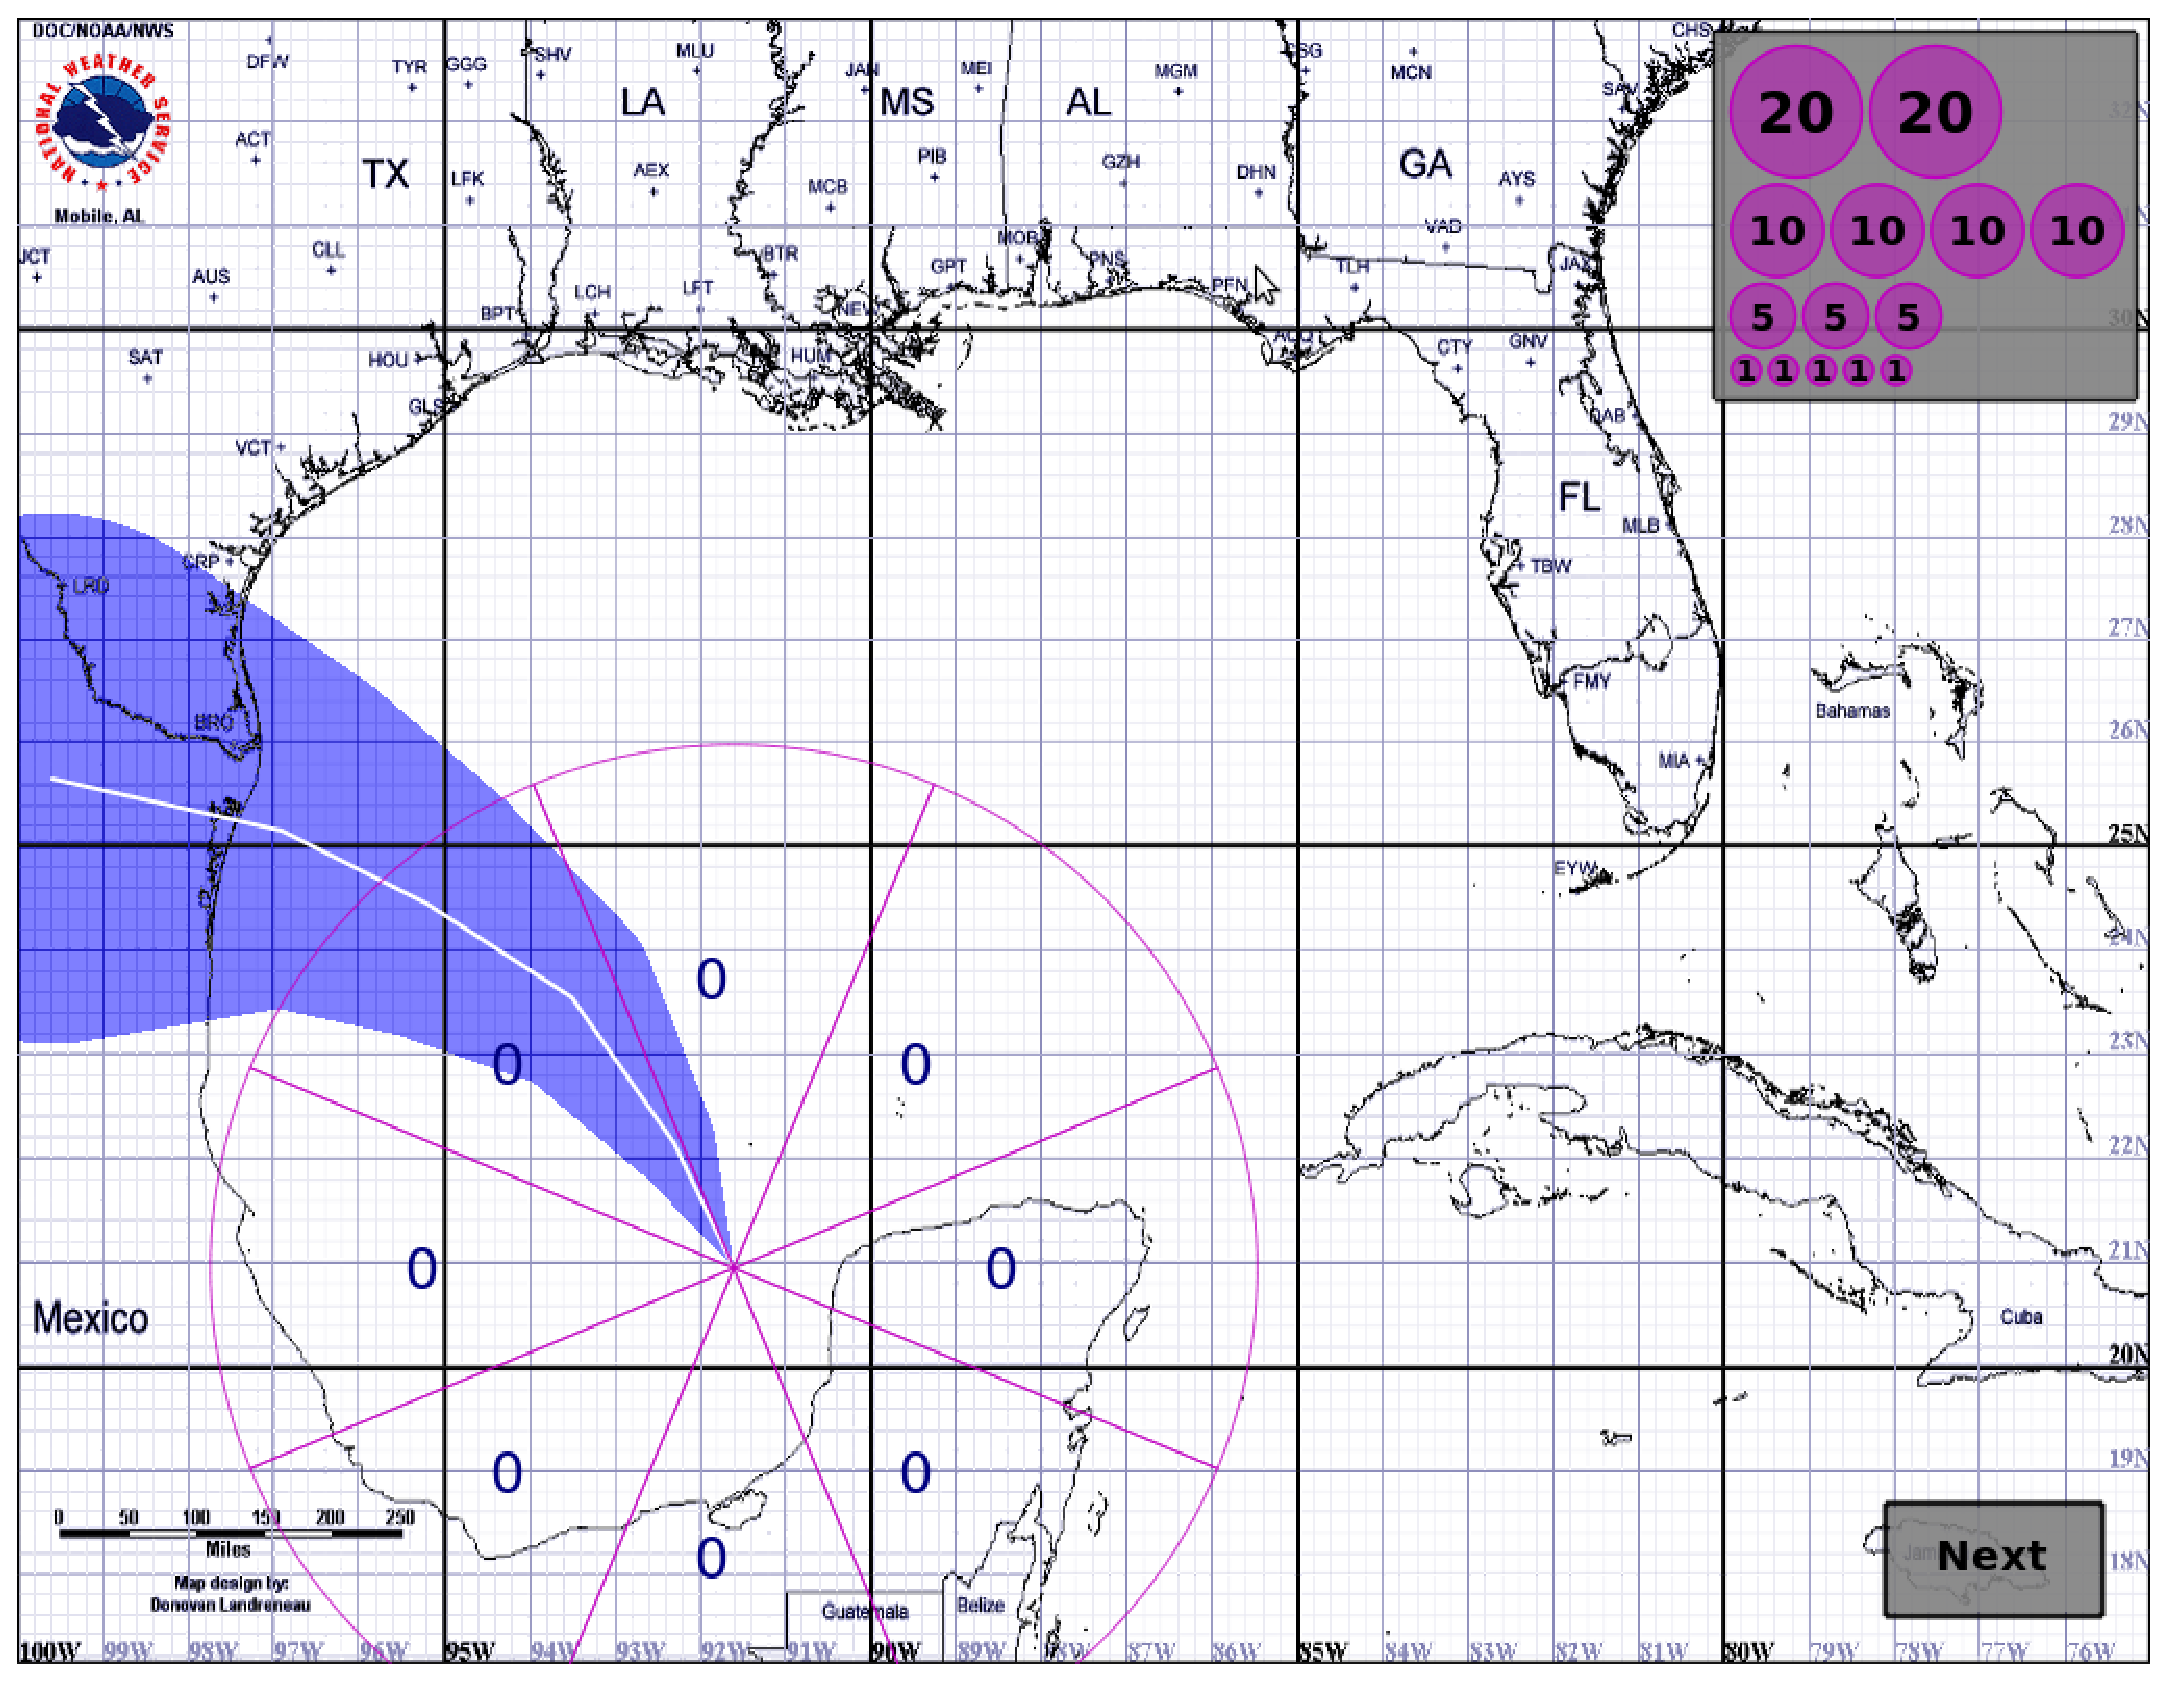
\includegraphics[width=2.0in]{figures/case_4_1.eps}
       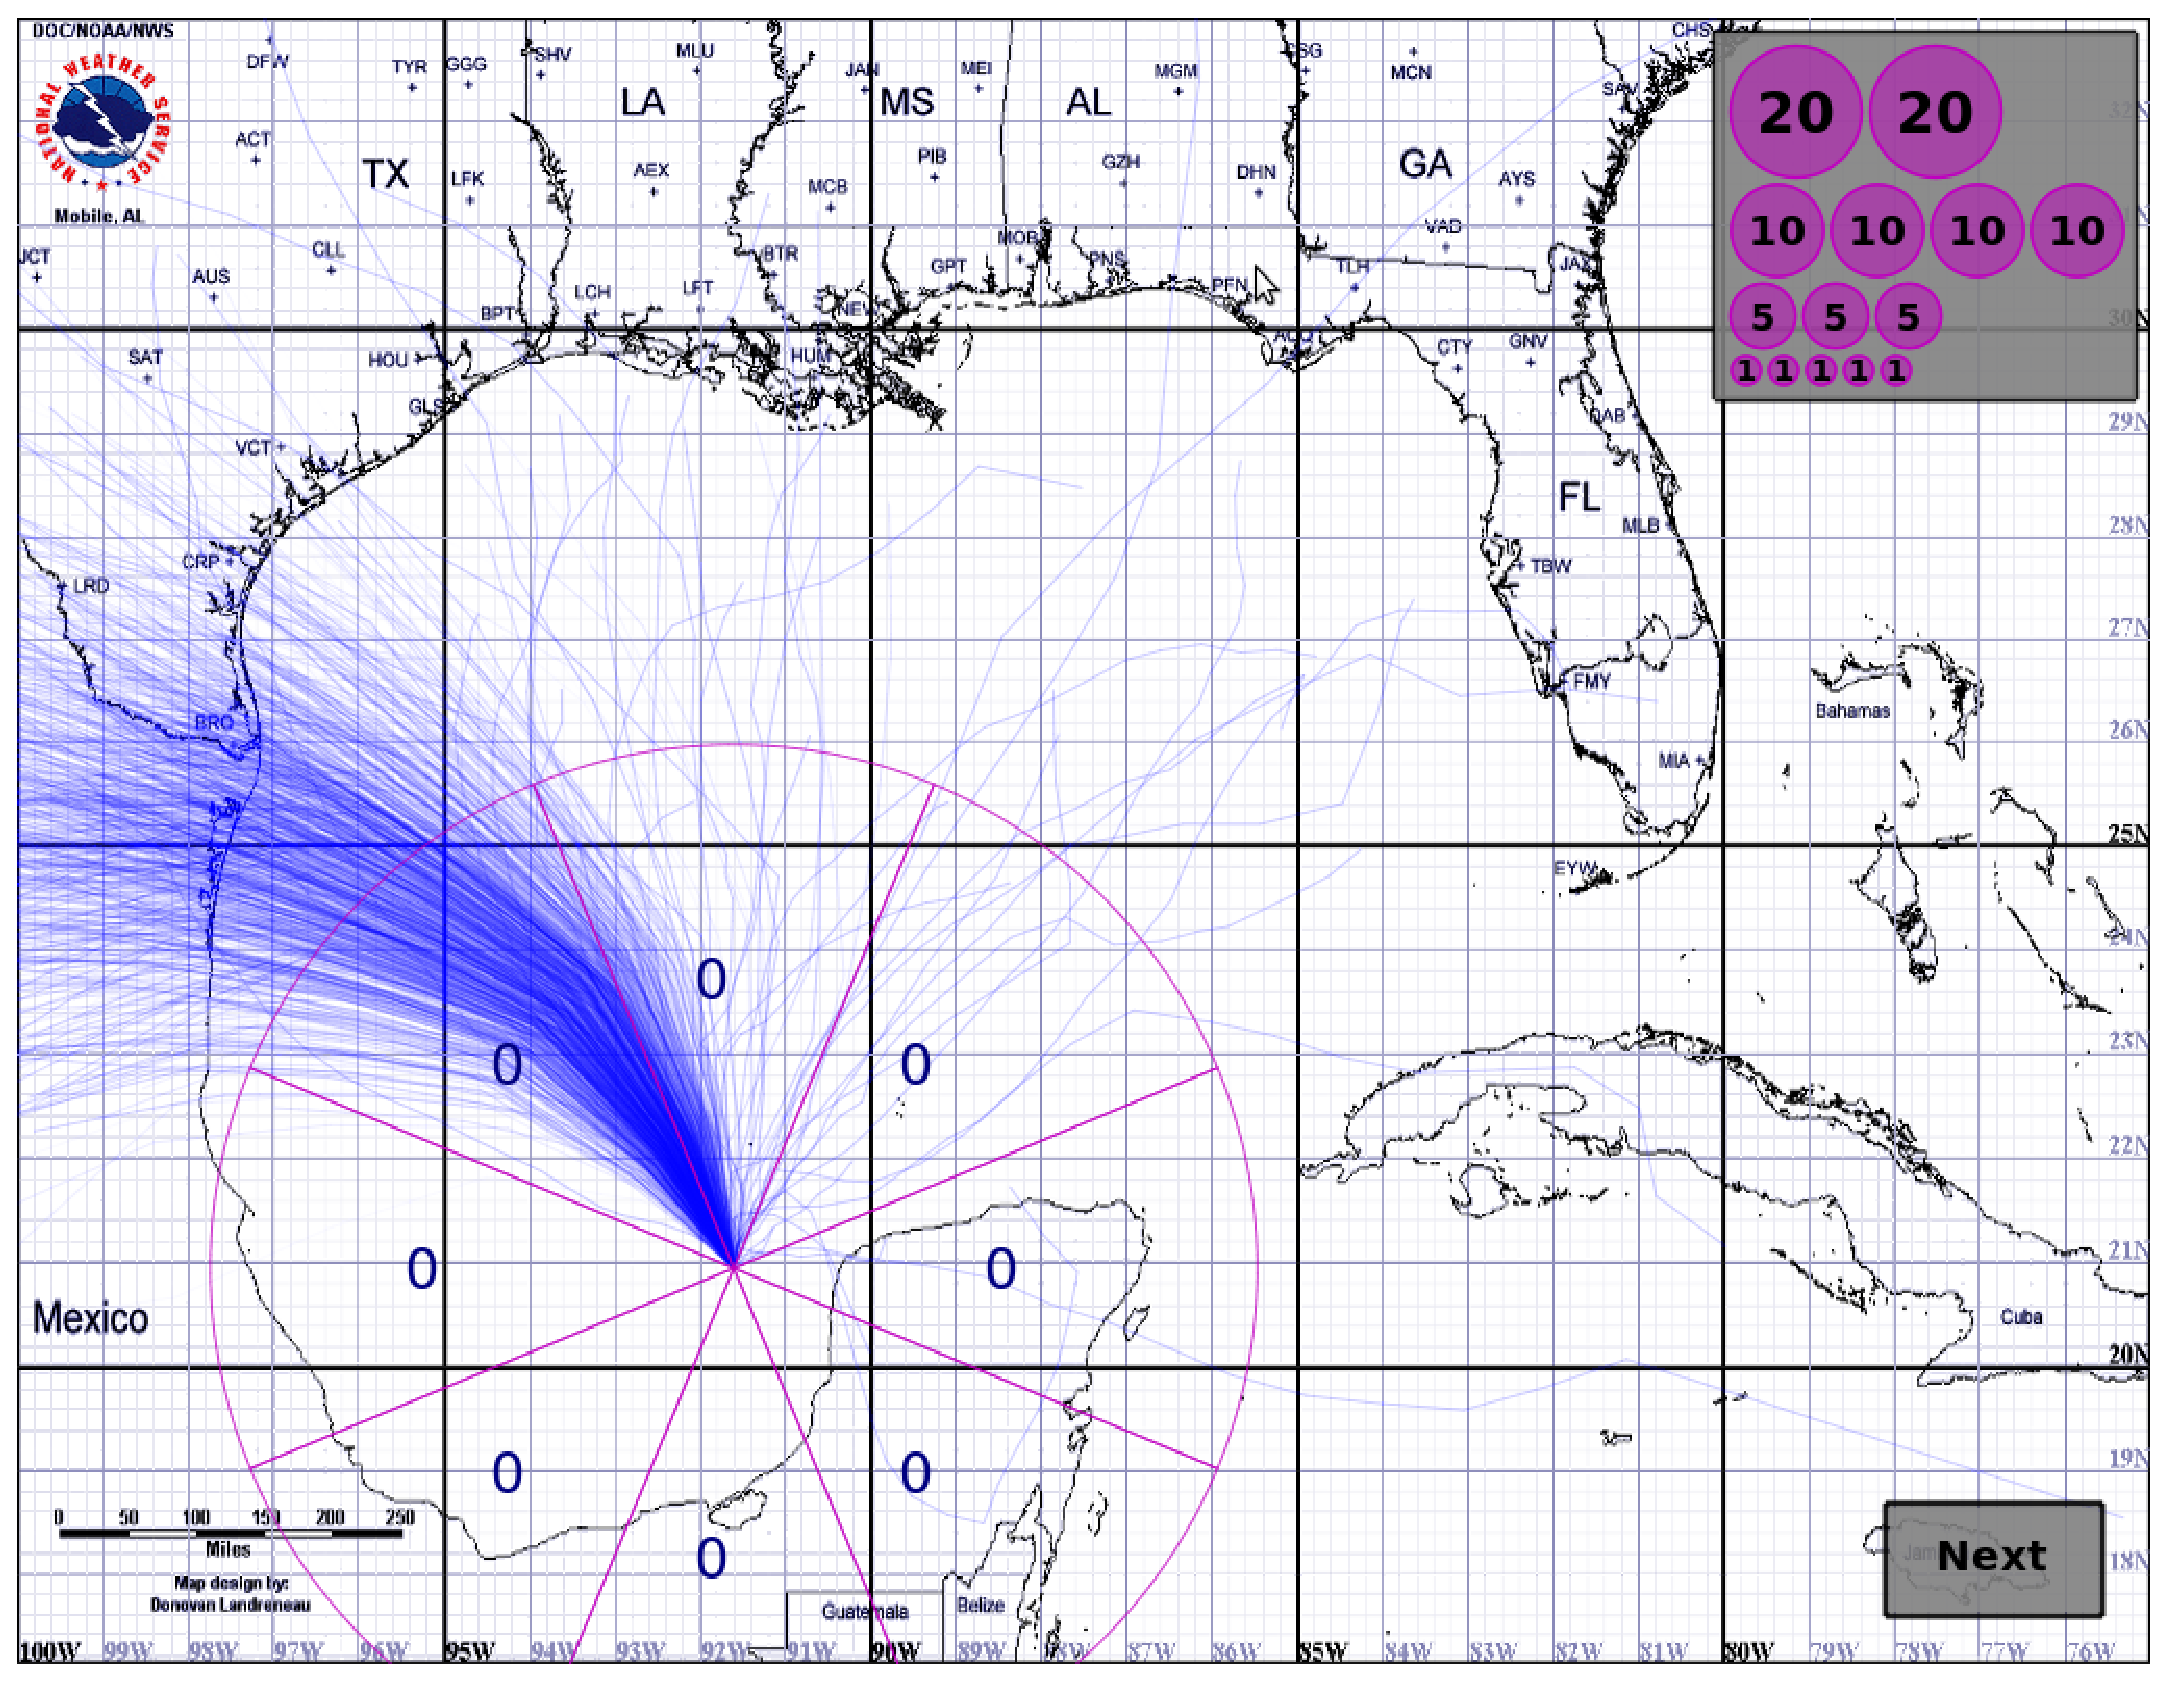
\includegraphics[width=2.0in]{figures/case_4_0.eps}
       \centerline{\small Case 4}}
       \hspace{1em}
    \parbox[b]{2in}{
       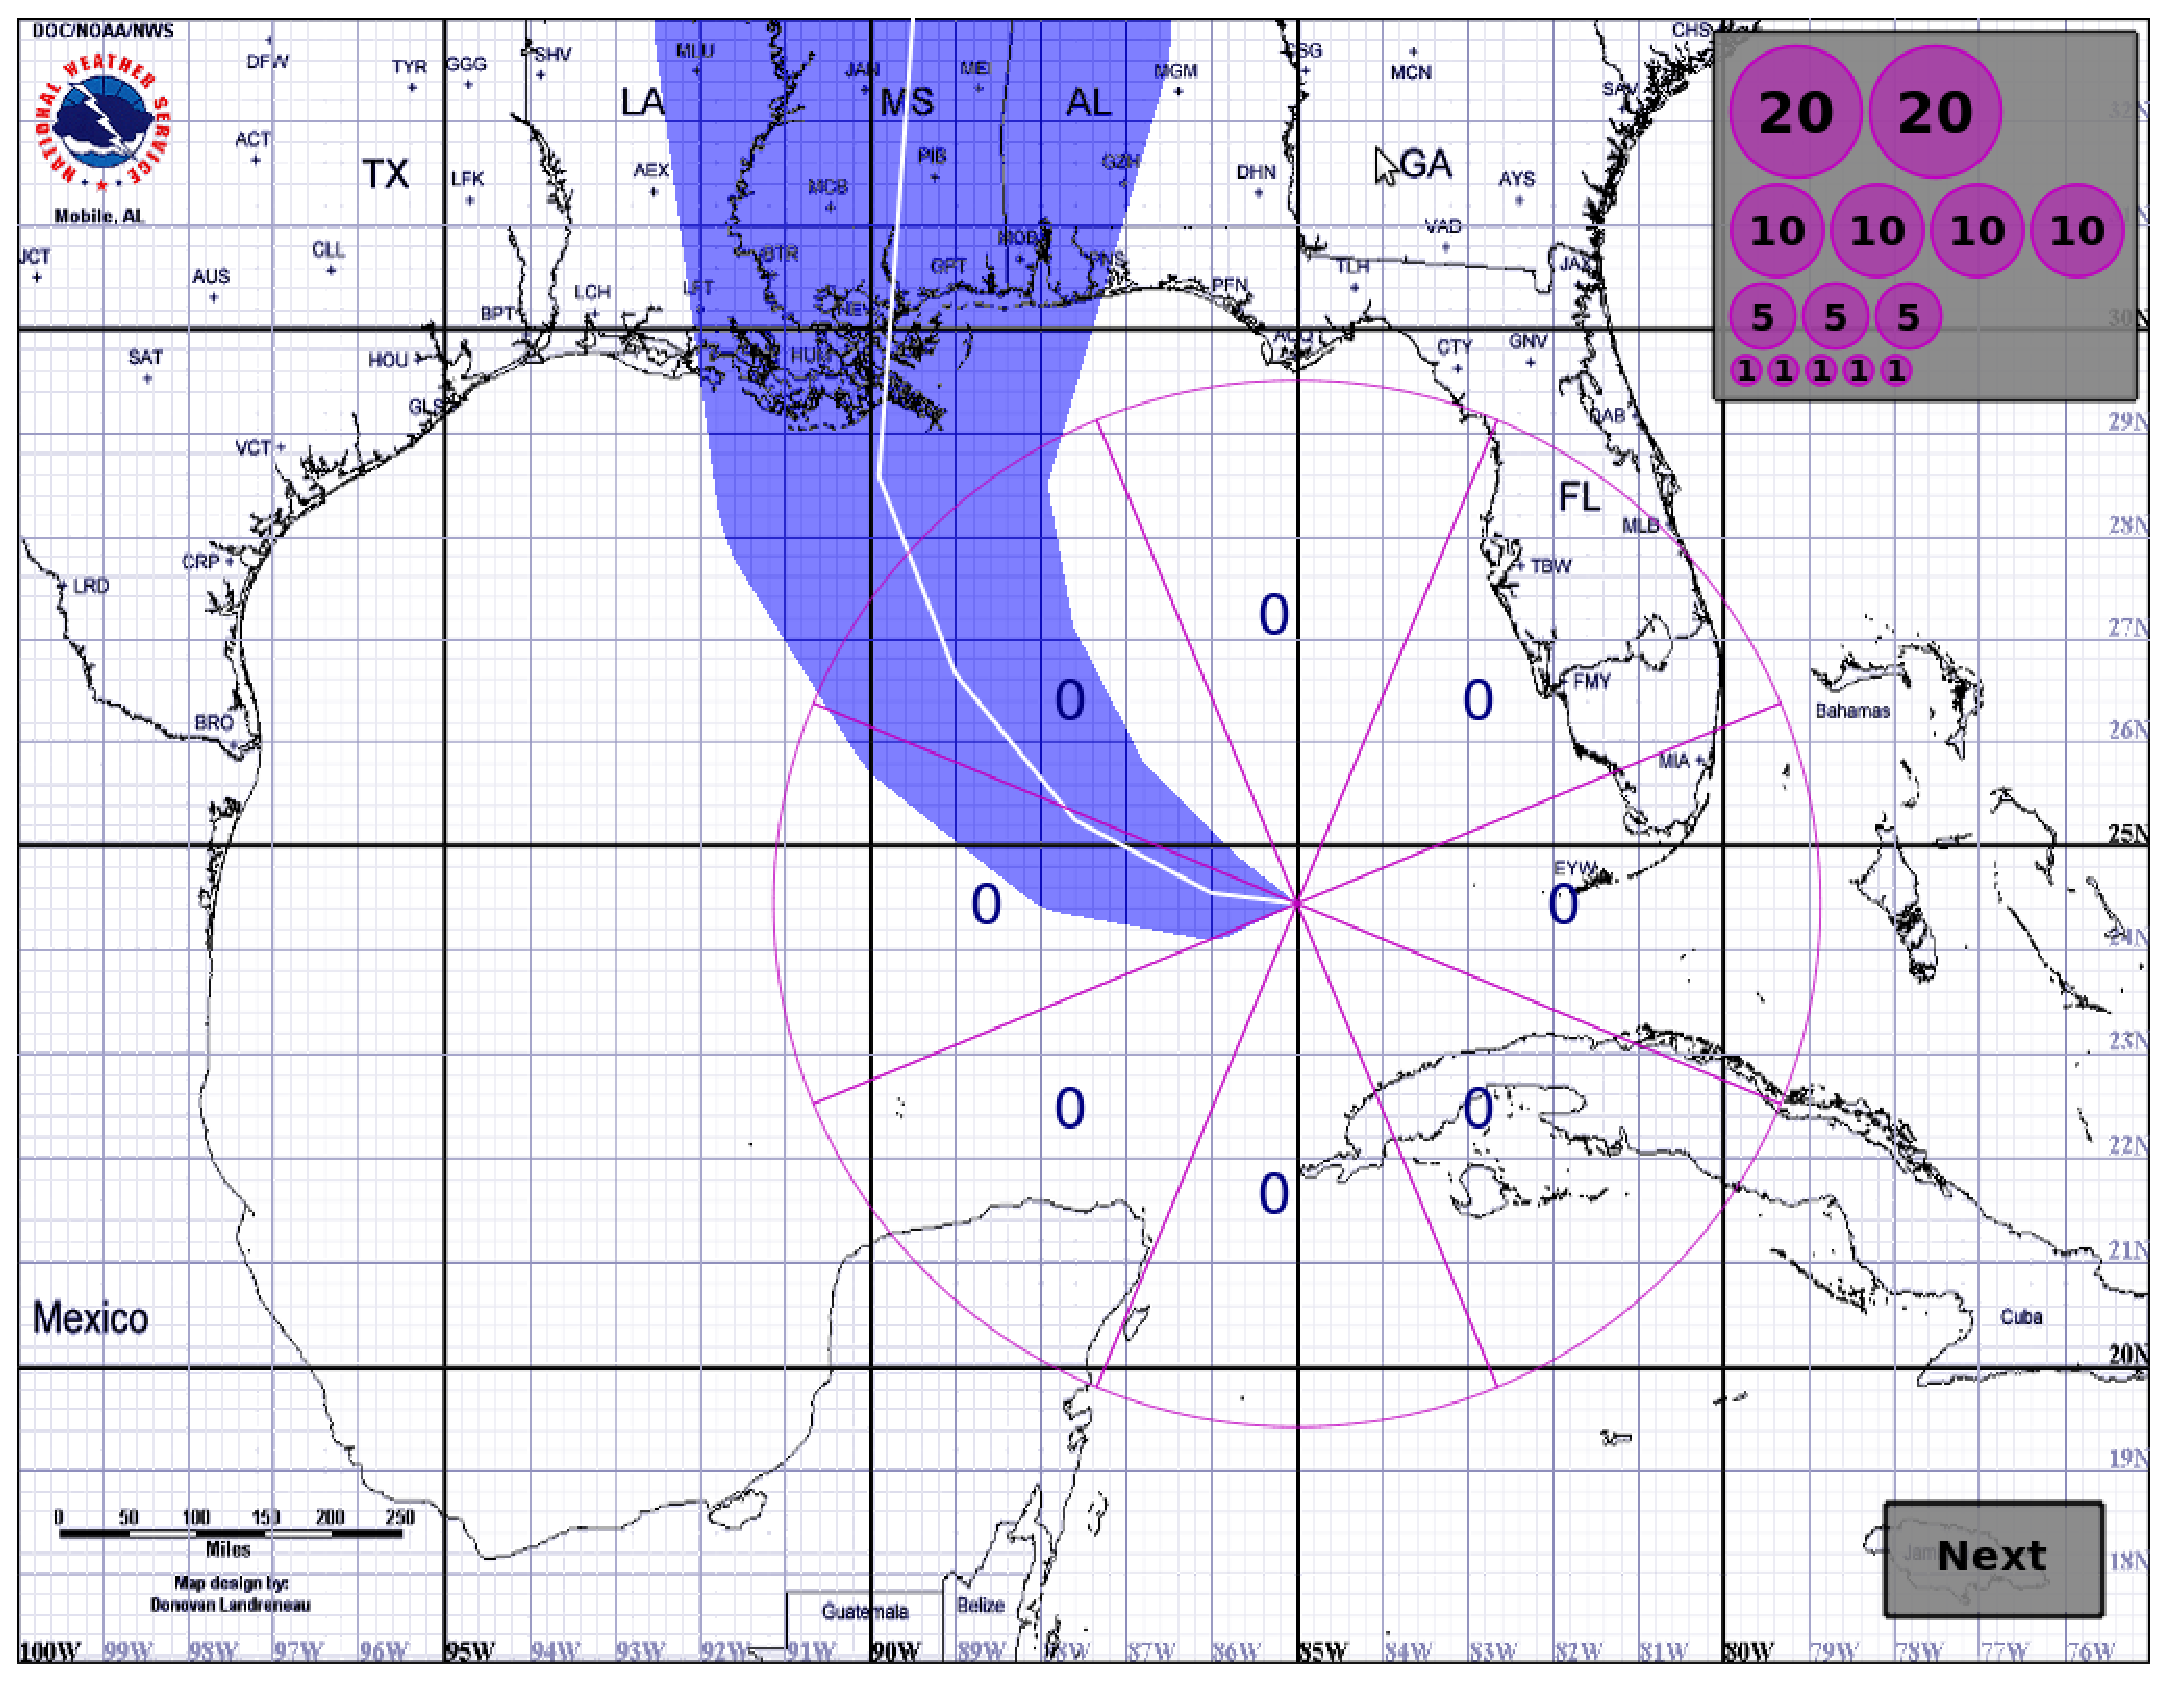
\includegraphics[width=2.0in]{figures/case_5_1.eps}
       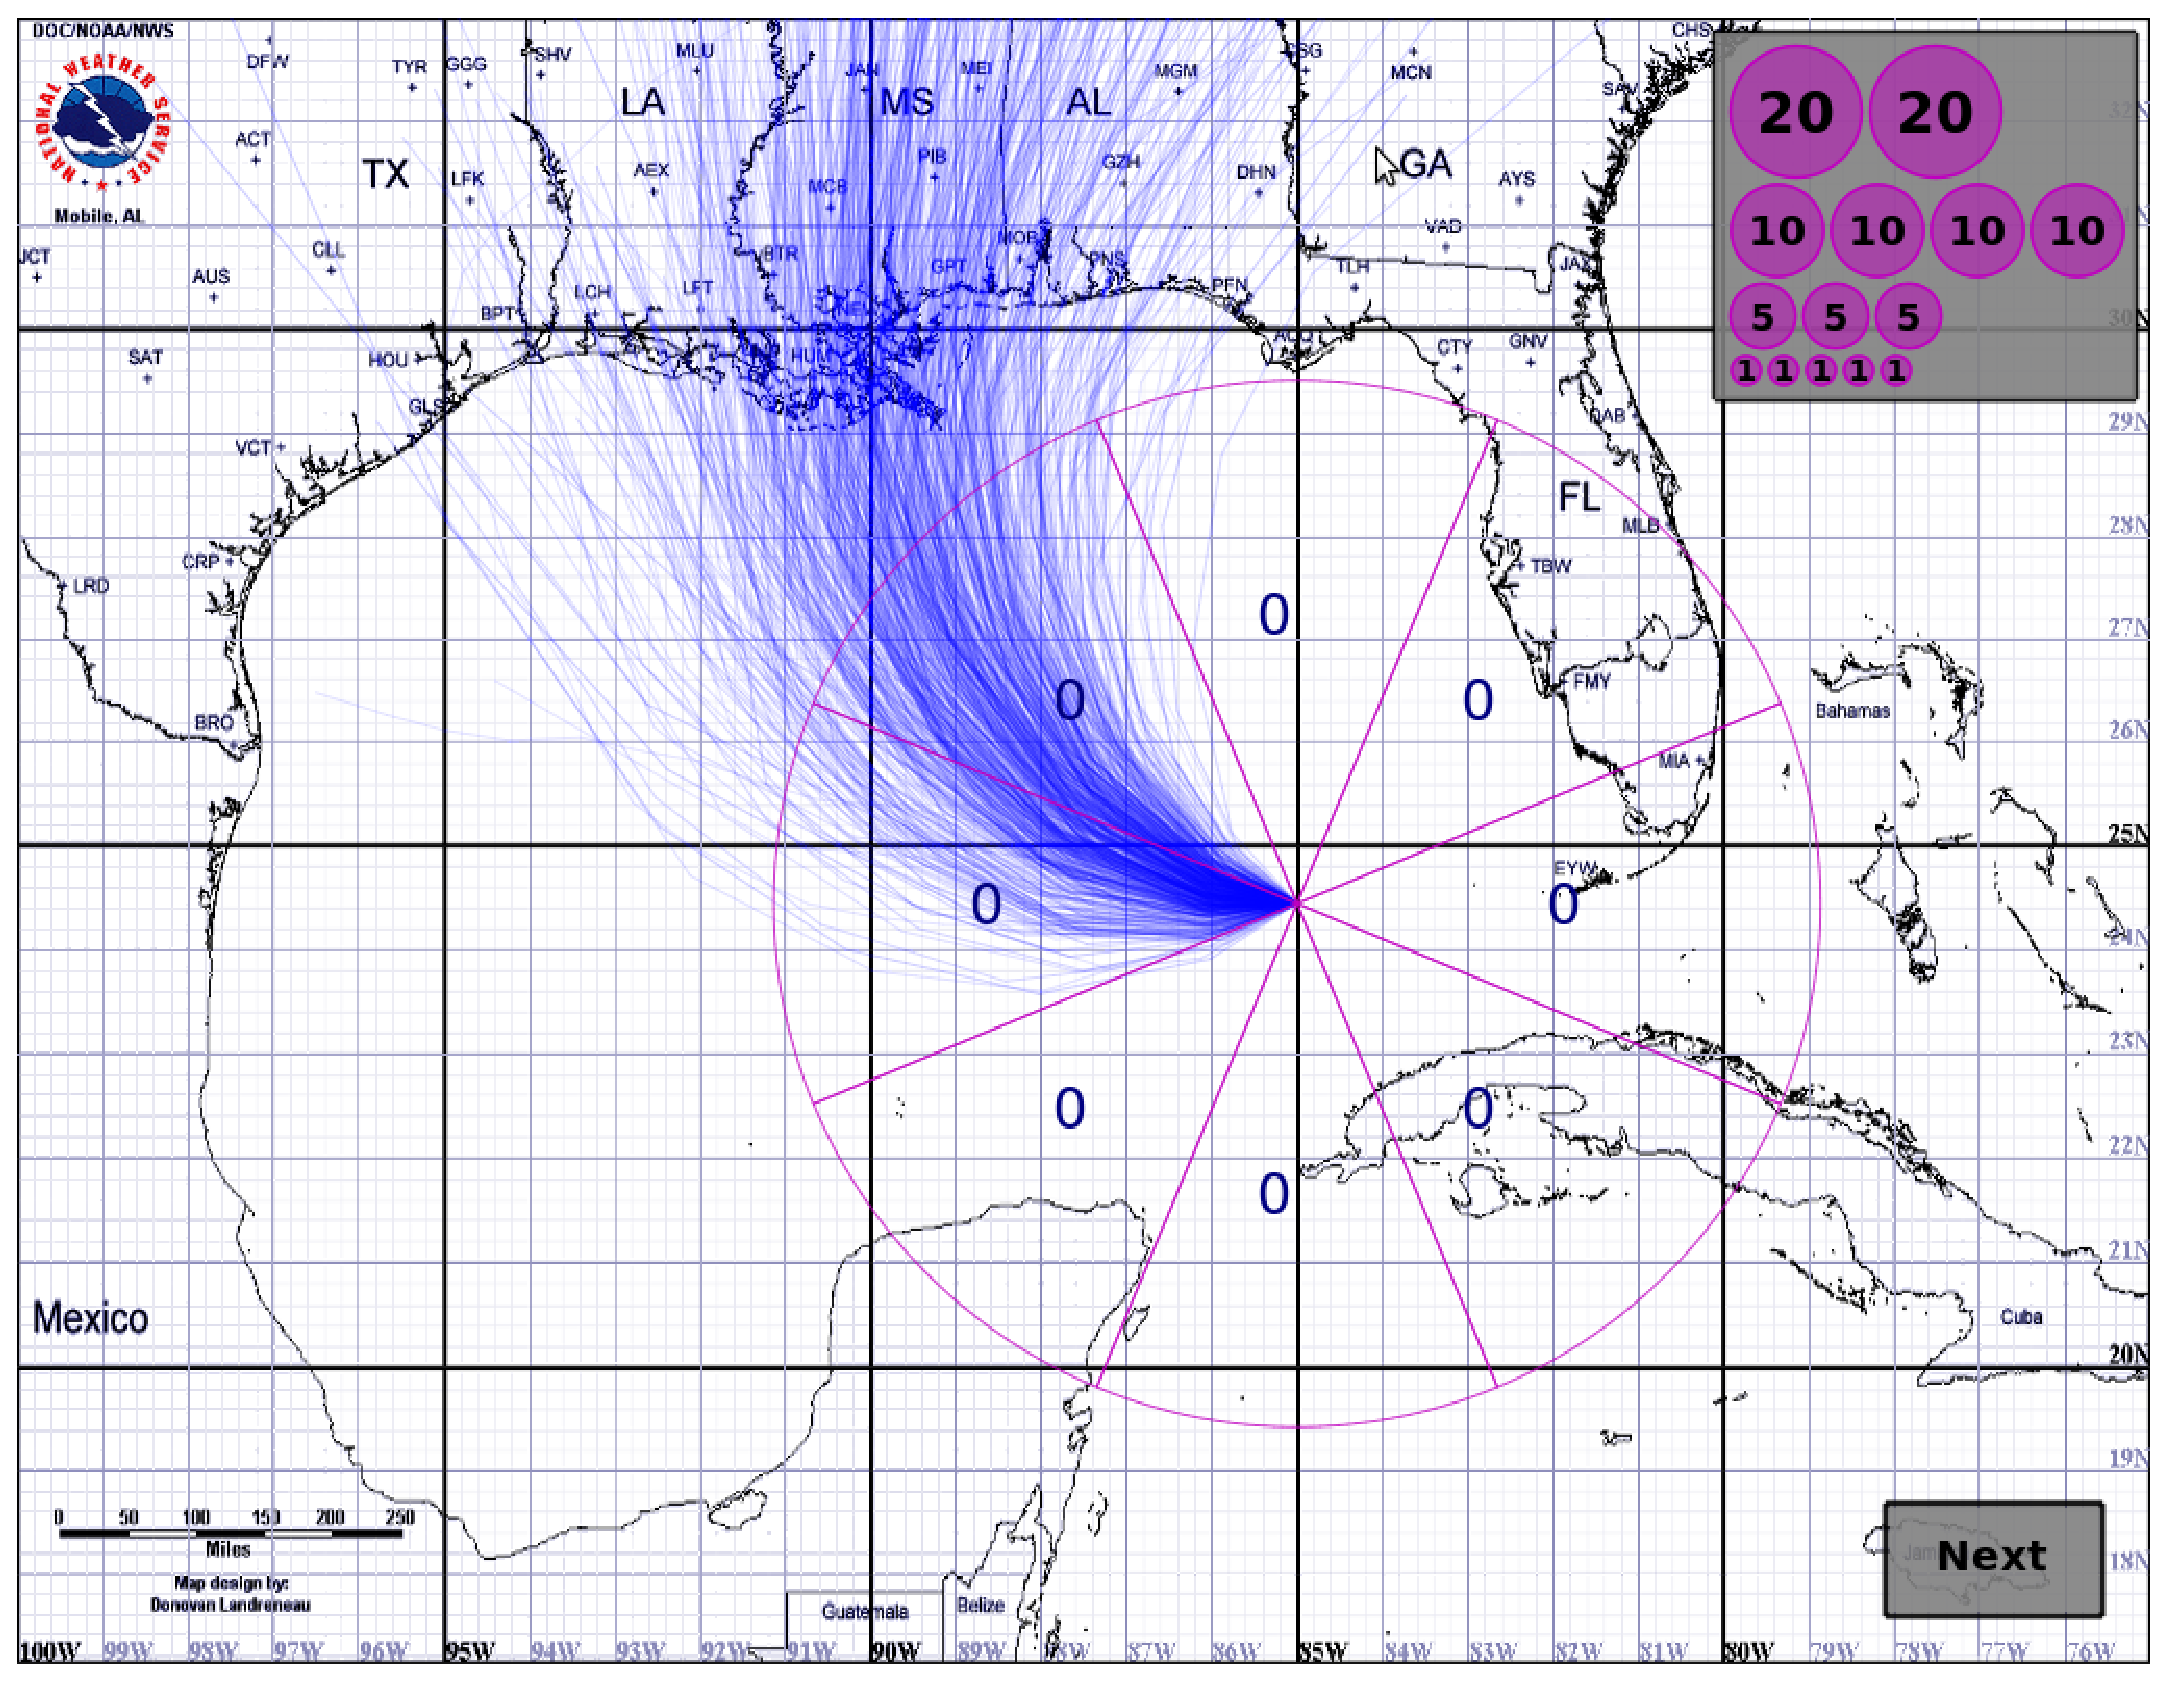
\includegraphics[width=2.0in]{figures/case_5_0.eps}
       \centerline{\small Case 5}}
       \hspace{1em}
    \parbox[b]{2in}{
       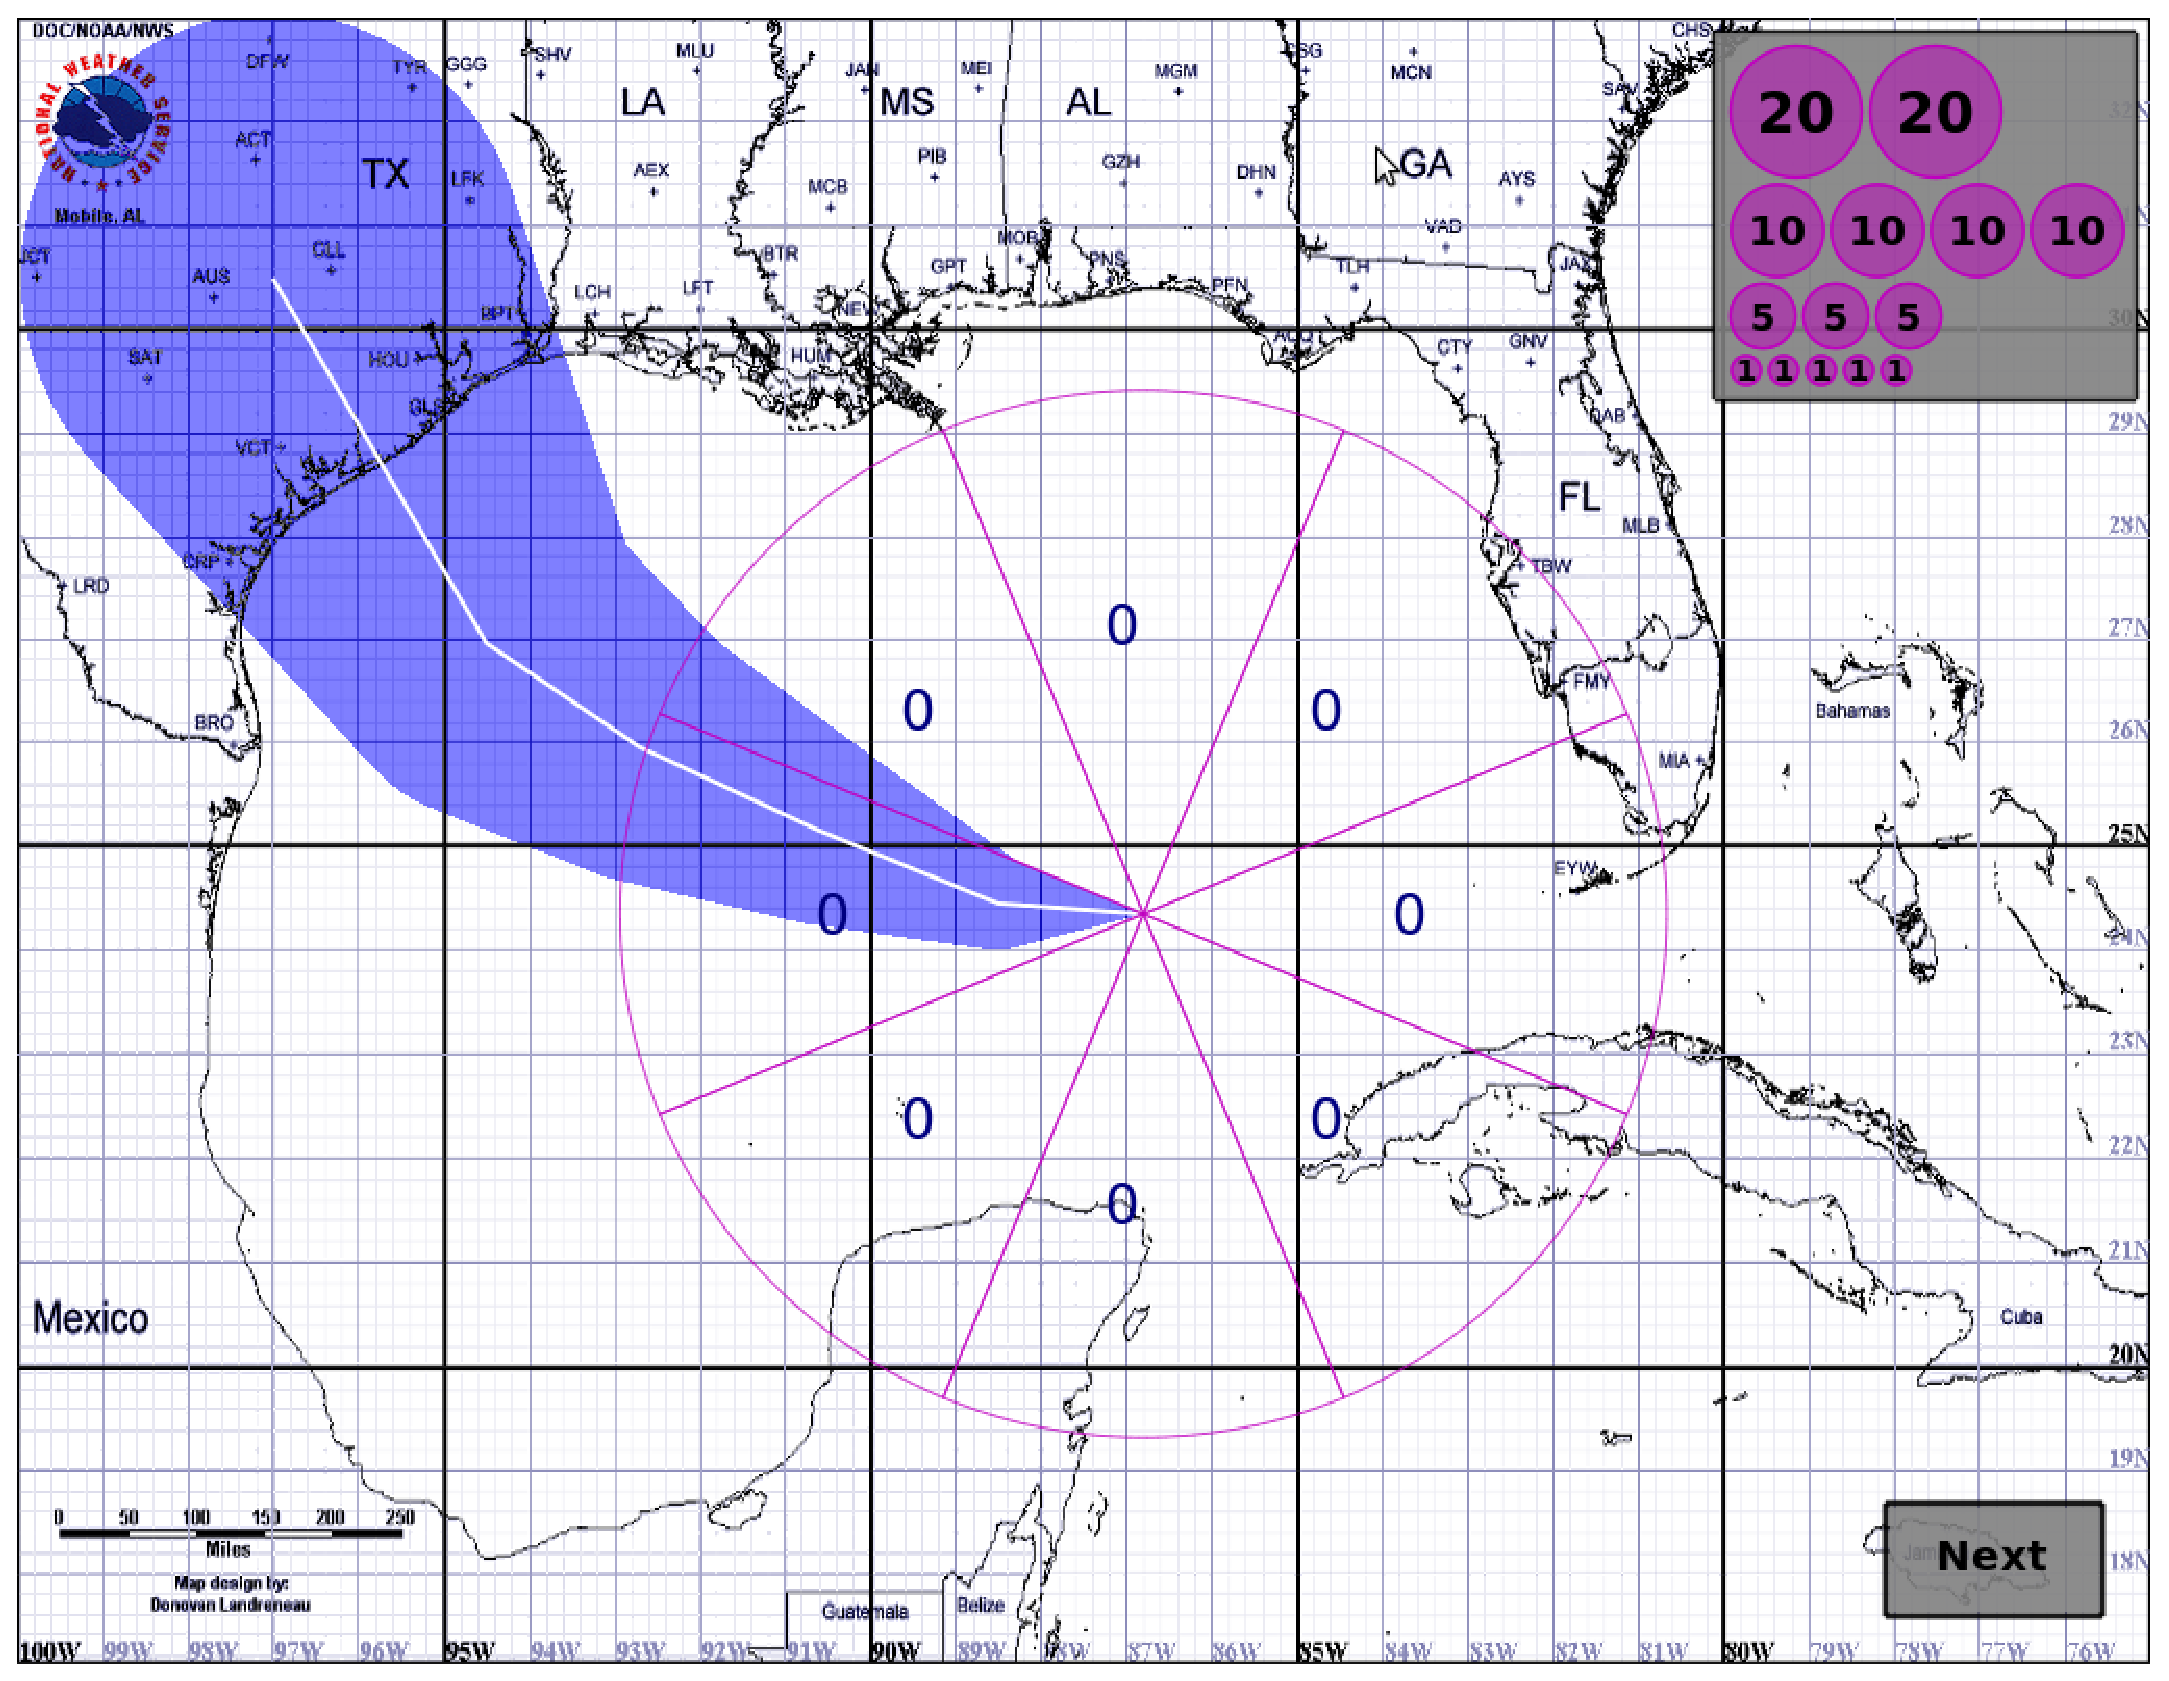
\includegraphics[width=2.0in]{figures/case_6_1.eps}
       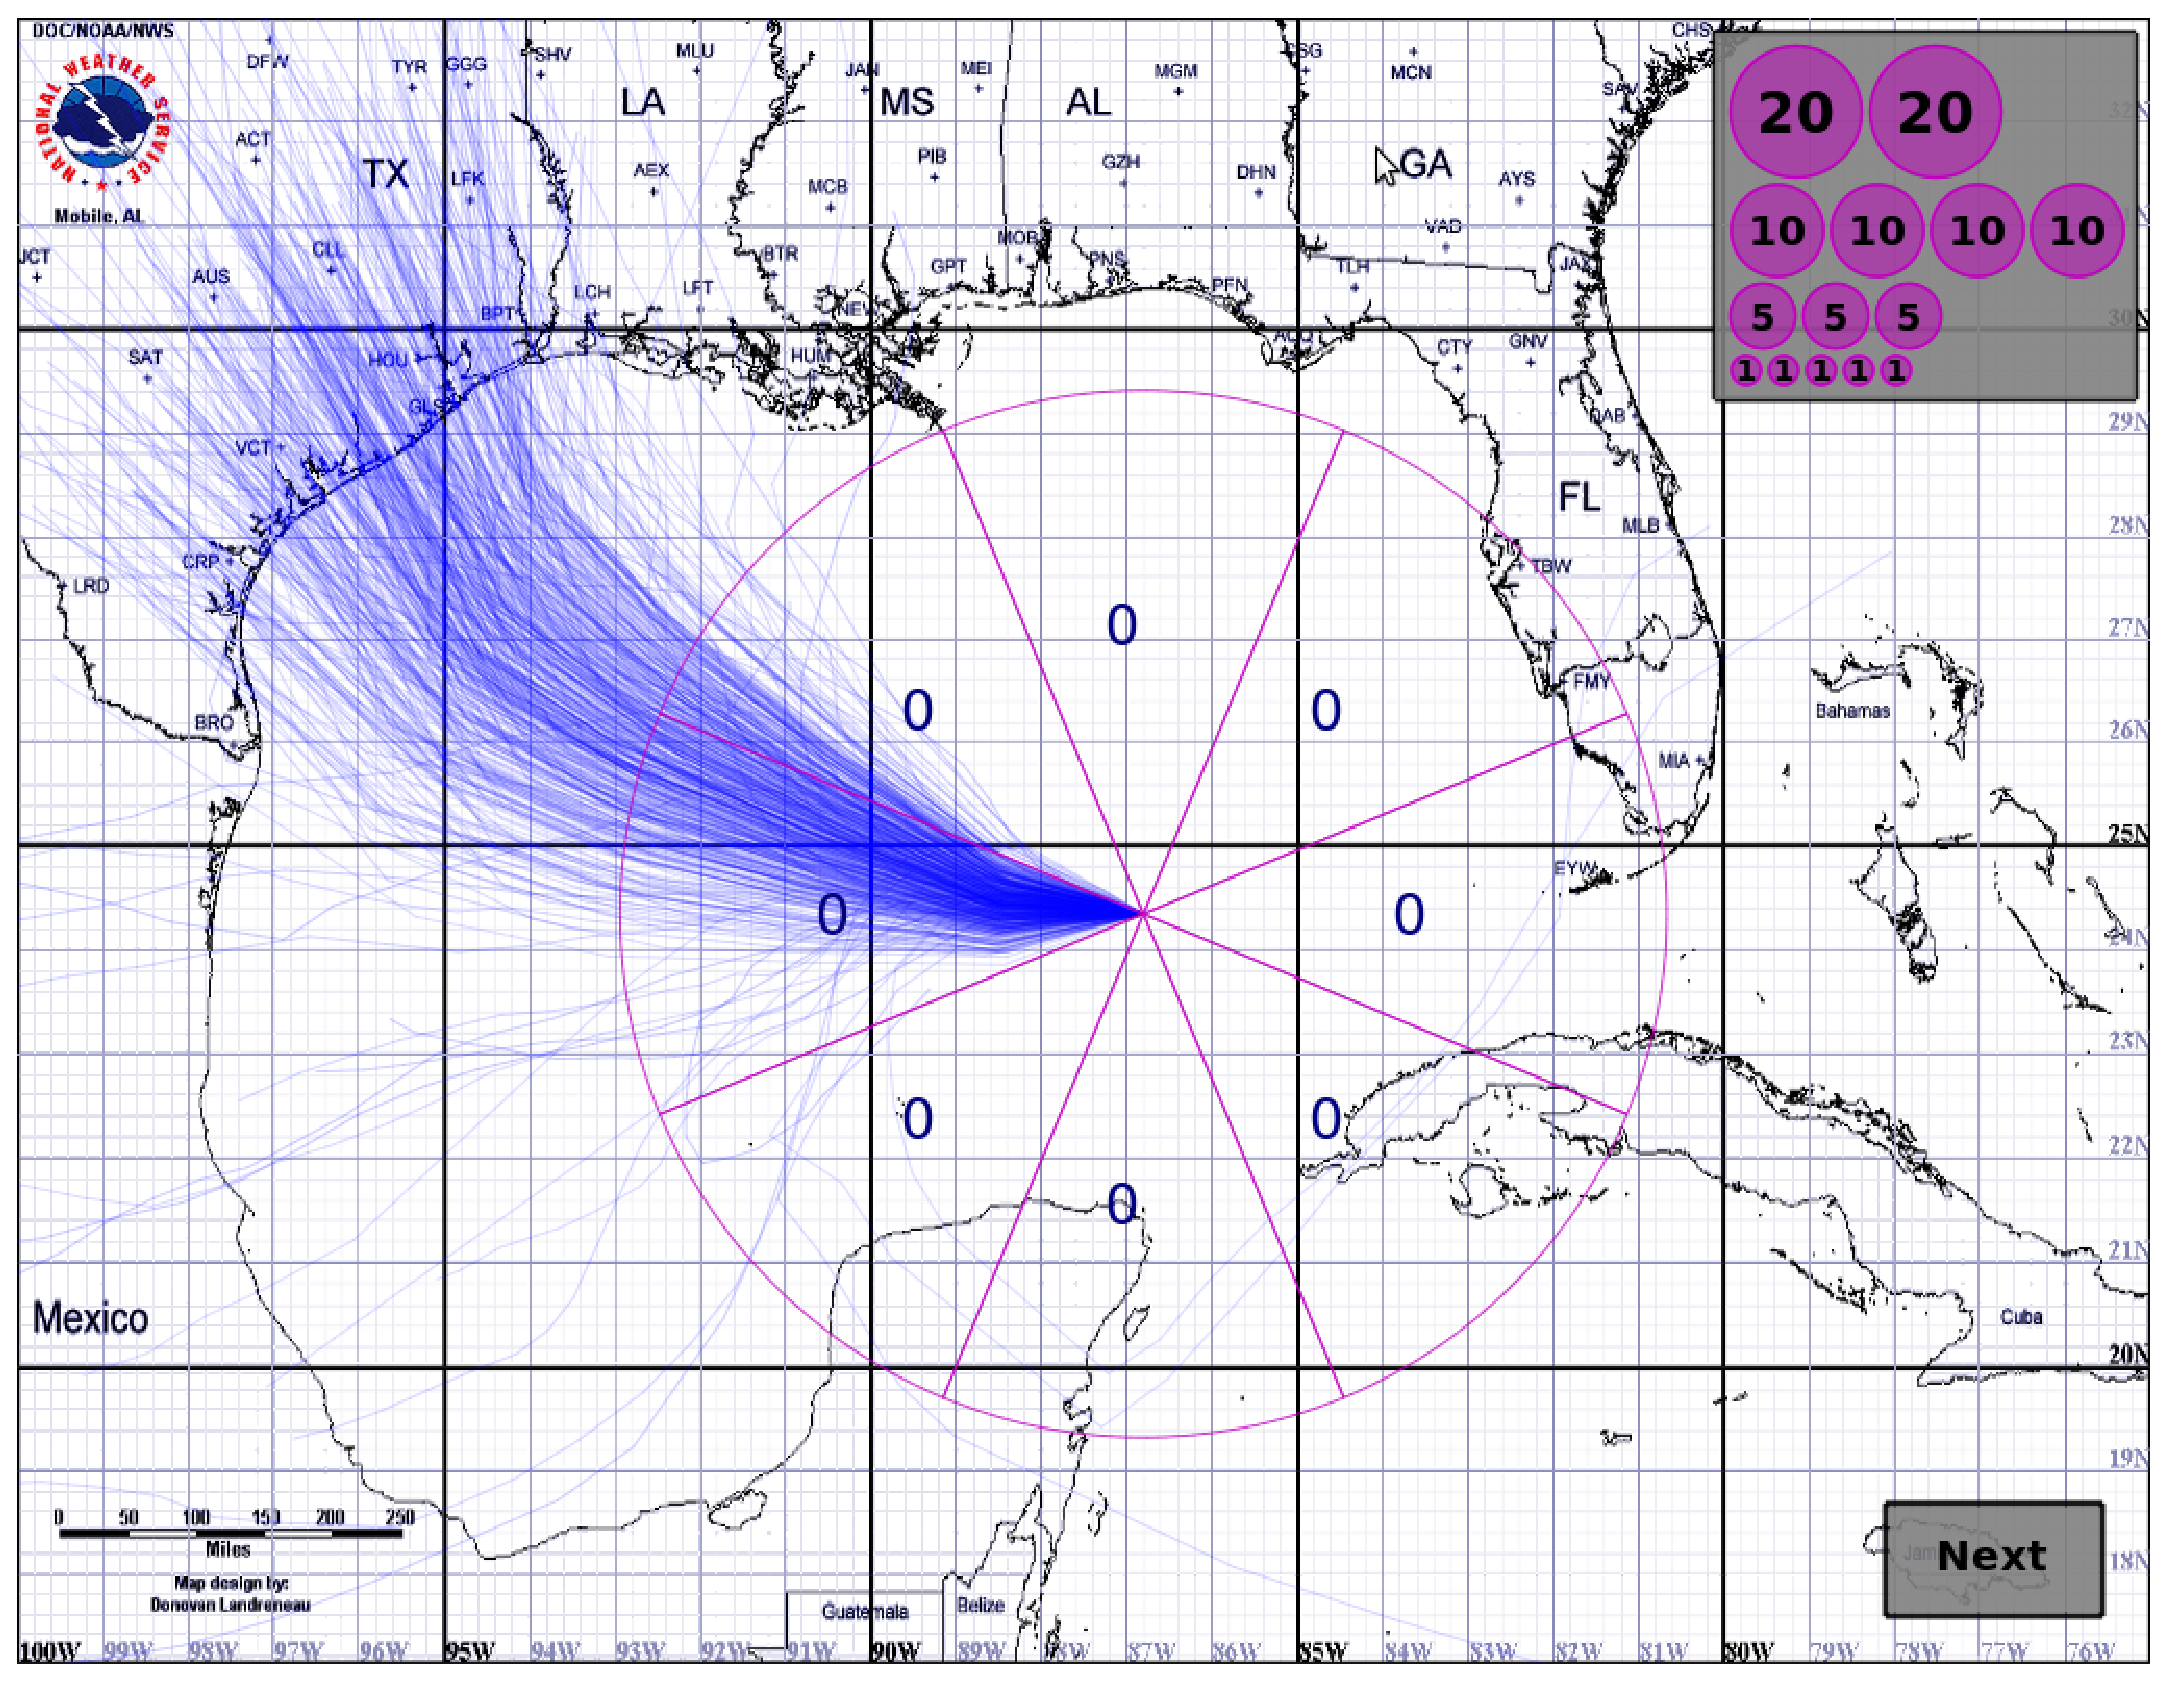
\includegraphics[width=2.0in]{figures/case_6_0.eps}
       \centerline{\small Case 6}} 
   }

 \caption{The Six Cases as Shown to Experiment Participants}
 \label{fig:6cases_comp}
\end{figure*}

We performed our statistical evaluation of the experimental results by first doing a profile analysis of the distribution of strike percentages across all of the sectors for each case, comparing results obtained with the error cone and our visualization method. The null hypothesis was that there should be no difference
in the distribution profile based on visualization method. We then ran a T-Test for each sector, for each case, to further isolate where
significant differences might lie. 

\begin{table}[htb]
  \caption{Profile Analysis and T-Test Results}
  \centering
  \includegraphics[width=3.5in]{figures/results_profile.eps}
  \label{table:profile}
\end{table}

Table~\ref{table:profile} summarizes the results of these analyses. 
The profile $p$ values for each case are shown in the bottom row, with $p$ values for each sector listed above them.
Cells colored red indicate no significant
difference ($p > 0.10$), cells colored blue indicate marginal difference ($p \le 0.10$), while cells colored green indicate significant
difference ($p \le 0.05$). 
Within the rows for the sectors, a solid box surrounds the sector or sectors, for each case, through which the error cone exits the circle. 
For example,
in Case 1 the error cone exits through both the North and Northwest sectors, while in Case 4 it exits only through the Northwest sector
(see Fig.~\ref{fig:6cases_comp}).

Turning first to the profile analysis, Cases 2, 3, 4, and 5 showed significant differences, while Cases 1 and 6 did not.
Fig.~\ref{fig:case_stat} provides a visual comparison of the profiles for Cases 1 and 4, confirming the results of the 
analysis. In this figure, sectors are on the horizontal axis, and the vertical axis shows the mean percentage assigned 
to each sector. 
The sectors are organized with sector 1 facing directly South, and continuing clockwise
so that sector 7 faces Southeast. It is interesting to note, from this figure, that the main source of difference in Case 4
is a wider distribution of strike probability, towards the East, with our visualization method than with 
the error cone.

\begin{figure*}[htb]
 \centering
 \hbox{
      \parbox[b]{3in}{
       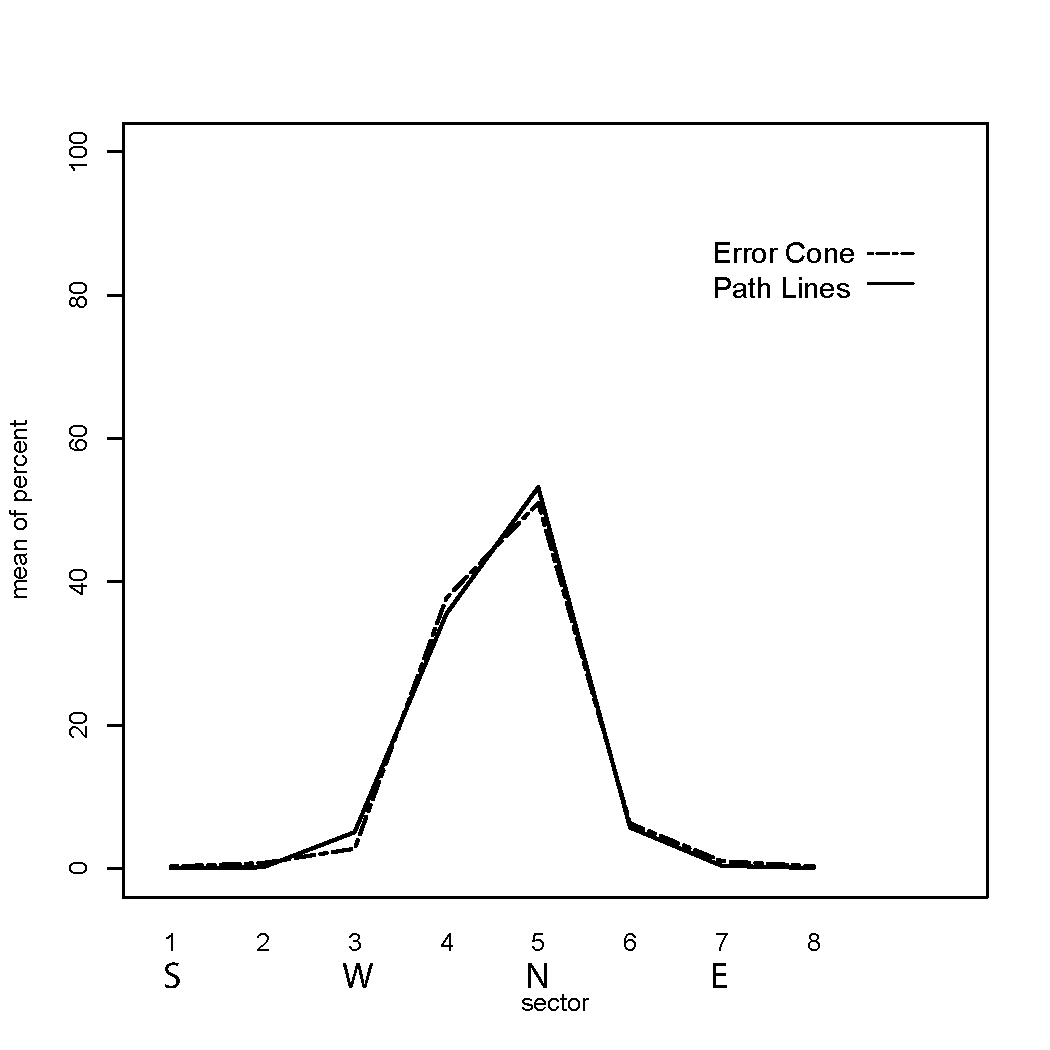
\includegraphics[width=3.0in]{figures/case-1.eps}
       \centerline{\small Case 1}}
       \hspace{1em}
      \parbox[b]{3in}{
       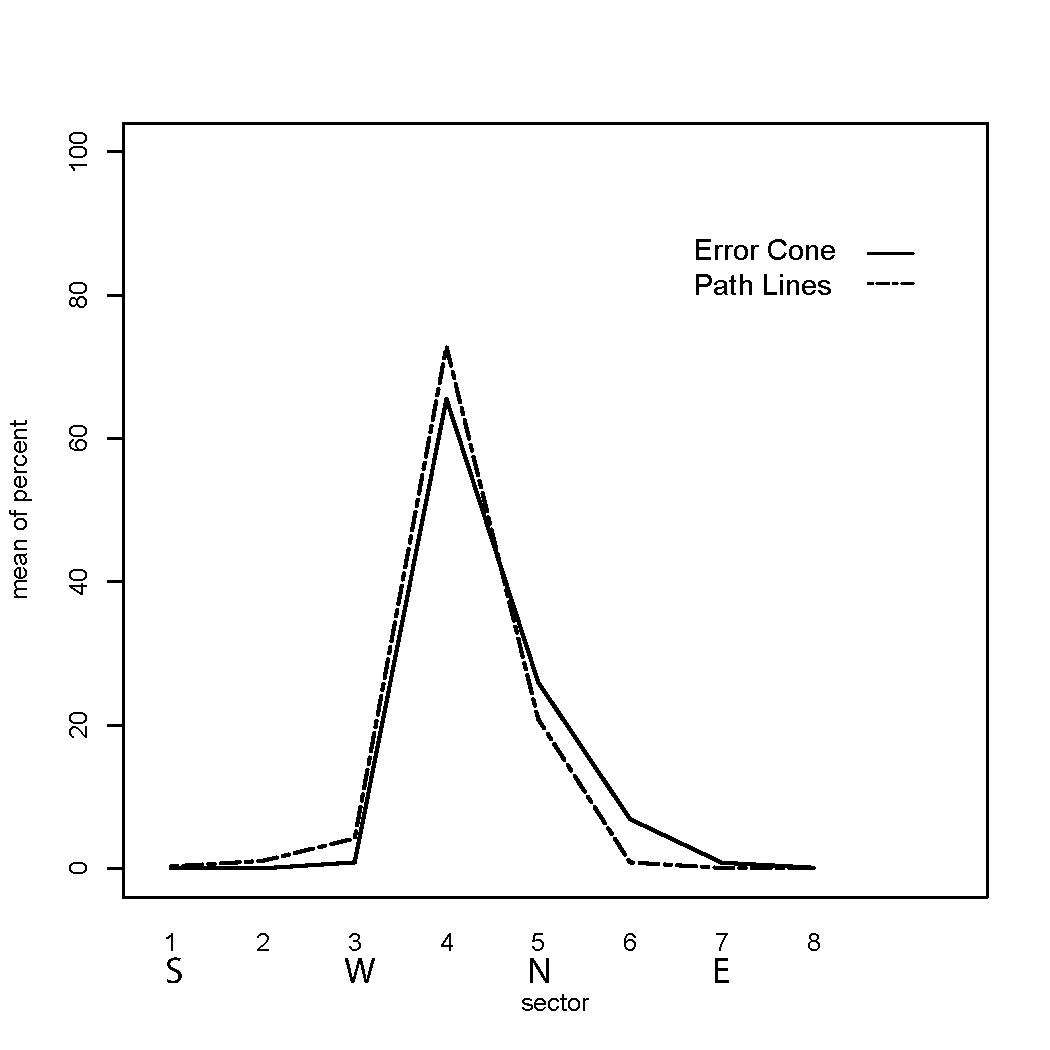
\includegraphics[width=3.0in]{figures/case-4.eps}
       \centerline{\small Case 4}}
}
 \caption{Profiles of two Hurricane Cases with Low and High Significant Difference}
 \label{fig:case_stat}
\end{figure*}

%A closer look at hurricane case one shows that the distribution of percentage points for both our visualization tool and the error cone was almost identical for all sectors, as can be seen in Fig.~\ref{fig:case_stat}.  When we do the same comparison for hurricane cases three and four, we can see that the participants gave a broader distribution of percentage points to the sectors, adding a few percentage points to the north and north east sectors.

Further inspection into these different cases revealed an interesting observation. In Cases 3 and 4, which showed the
strongest profile differences,  the error cone stayed almost entirely within a single sector and exited entirely within that sector. For the rest of the cases, the area of the error cone was more evenly split between two adjacent sectors. This leads us to speculate that an additional study with a more fine grained structure may be needed to determine the overall significance of the difference between the two visualization methods.

%Based on a statistical analysis of the data resulting from the experiment, we were unable to conclusively determine whether our method increased an individual's understanding of the uncertainty associated with a predicted hurricane track compared to that of the error cone.
Finally, we looked at the mean direction for each case, as shown in Fig.~\ref{fig:dirMean}. The blue line on the figure
shows the direction of the center line of the error cone, as it crossed the circle boundary. We see that overall trend in mean direction across all cases, and for both visualization methods, closely matches the expected mean direction.
However, for our method, Cases 3 and 4 shift towards the North, while both methods shift towards the West for Case 5.
For Cases 3 and 4, the North shift can be explained by the influence of historical trends in our visualization. 
Historically, central Gulf hurricanes headed Northwest tend to veer towards the North and Northeast. We expect
that the shift to the West in Case 5 is due to the fact that the hurricane prediction starts out almost wholly in the West
facing sector and then shifts later to the Northwest, exiting almost wholly in that sector. It may be that participants
ignored which sector the hurricane exited the circle in, and instead considered the entire path.

\begin{figure}[t]
 \centering
   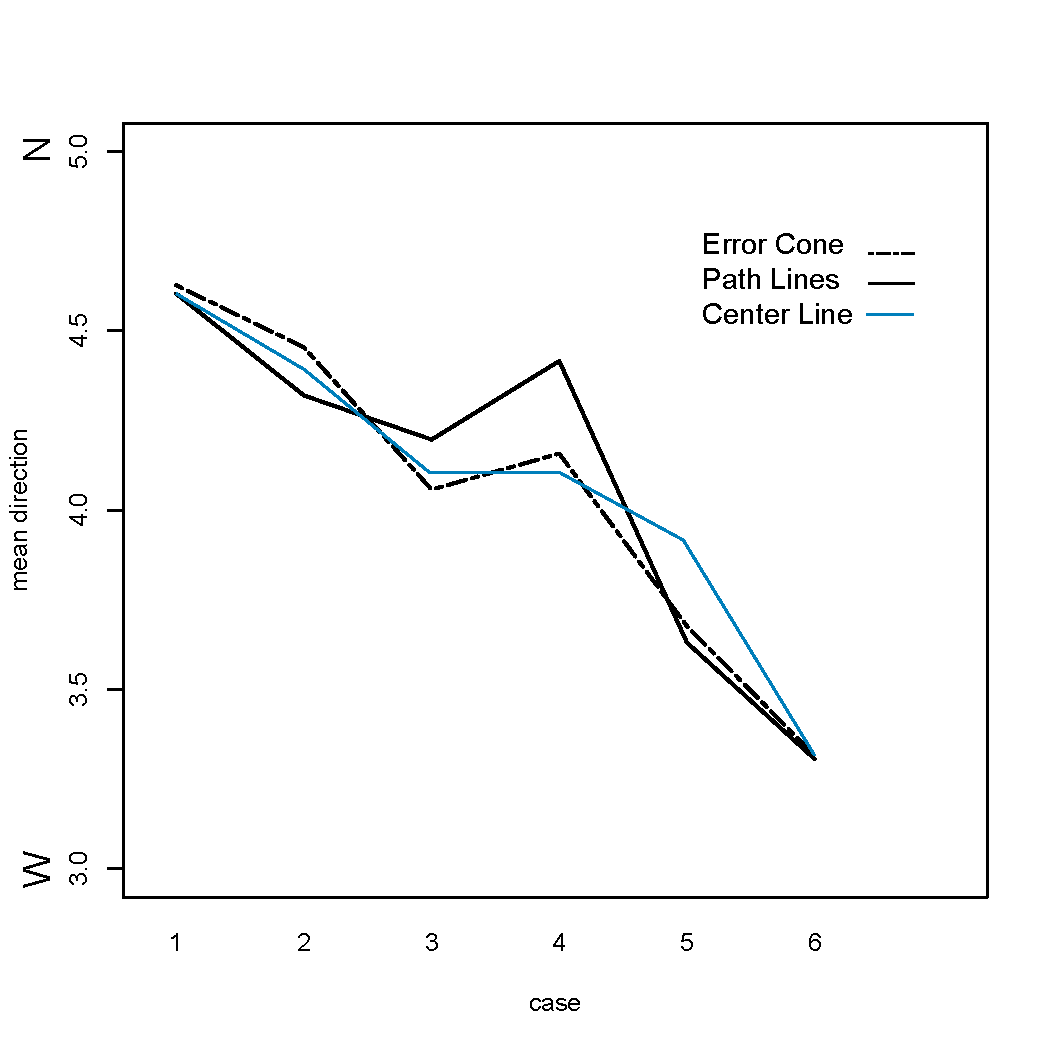
\includegraphics[width=3.0in]{figures/mean-plot.eps}
  \caption{Direction Means}
 \label{fig:dirMean}
\end{figure}

The results of the qualitative analysis were quite clear.  On the paper and pencil questionnaire, only one participant out of 23 indicated that they slightly preferred the error cone, with a score 4.  All other responses were either a strong preference for our method with a score of 1, or a slight preference, with a score of 2.  The mean score over all of the participants was 1.56, and the standard deviation was 0.53.

The participants open ended feedback suggests that our method gave the users a better overall understanding of the uncertainty and unpredictability associated with forecasted hurricane tracks.  One consistent criticism of our method was that while it was more visually interesting to watch and provided a better insight to the dynamic behavior of hurricanes, it was also cognitively more difficult to work with than the error cone.

\section{Conclusion}

We have presented a visualization method as an alternative to the error cone display produced by the National Hurricane Center. 
Our method presents an ensemble of continuously updated tracks demonstrating the range of possible hurricane outcomes. It
uses both a hurricane's current advisory information and data on historical hurricanes to create a dynamic display showing the variety of possible hurricane tracks.  This approach produces tracks that lie both inside and outside the error cone, while maintaining statistical characteristics similar to those underlying the hurricane advisory. Our experimental study showed that there are differences between estimates of spatial distribution probability made when using
the error cone and our visualization method. However, these differences lie in the breadth of the distribution, and not in the mean. Thus, we can conclude
that our method does not mislead users into making incorrect estimates of the most probable direction of a hurricane strike, and may help them to better
understand the variance inherent in the prediction. Therefore, we conclude that there is justification for further study of this new visualization method, 
particularly with an emphasis on its use in making more fine-grained strike estimates.

Future work will include refining the algorithm, running additional user studies to investigate the how users perceive the uncertainty of a predicted hurricane track related to areas within the error cone and for particular geographical locations, and using our method as a base to support other visualization tools.  One idea is to generate a heat map from the generated tracks, and use it create a three dimensional display that describes the probability of a hurricane track in terms of a height field. This could be displayed in a 3D view, or a section through this view, following the coastline, could be displayed in 2D. Another possible visualization would be to superimpose our method over the error cone, so that both summary statistics and detailed outcomes can be viewed. We would like to explore methods to incorporate other important hurricane information, such as wind speed and storm shape, into the display. Finally, it would be useful to design a tool to assist in evacuation decision making, which would require integrating evacuation and hurricane models.



%% The Acknowledgements part is started with the command \acknowledgements;
%% acknowledgements are then done as normal sections before appendix
%% \acknowledgements

\acknowledgments{
This work was supported in part by NSF and NOAA under grant NSF CHI 2008001386.}


%% The Appendices part is started with the command \appendix;
%% appendix sections are then done as normal sections and after Acknowledgements
%% \appendix

%% \section{}
%% \label{}

%% References without bibTeX database:

%\begin{thebibliography}{-8}

%% \bibitem must have the following form:

%\small{
%\bibitem{key}

%...

%}

%\end{thebibliography}

\bibliographystyle{abbrv}
%%use following if all content of bibtex file should be shown
%\nocite{*}
\bibliography{hurricane}
\end{document}
